% ═══════════════════════════════════════════════════════════════════════
\section{Des monstres aux modèles}
% ═══════════════════════════════════════════════════════════════════════

\subsection{La fonction de Weierstrass}

\begin{frame}{Une fonction continue dérivable nulle part (1872)}
  \small Jusqu'au milieu du \siecle{19}, on tient pour acquis qu'une
  fonction continue est dérivable, sauf en quelques points isolés. Le
  18 juillet 1872, Weierstrass présente
  \[
    W(x) = \sum_{n=0}^{\infty} a^n\cos\big(b^n\uppi x\big),
    \qquad 0<a<1,\ b \text{ entier impair assez grand.}
  \]
  \begin{itemize}
    \item Chaque terme est lisse ; la série est majorée par $\sum a^n$,
      et sa somme est continue.
    \item Pourtant $W$ n'est dérivable en aucun point (Hardy, 1916 :
      $ab\geq1$ suffit, d'où $a=\tfrac12$, $b=3$).
    \item Des amplitudes $a^n$ qui décroissent, des fréquences $b^n$ qui
      croissent beaucoup plus vite : des oscillations de plus en plus
      petites mais de plus en plus raides ; la pente ne se stabilise
      jamais.
  \end{itemize}
\end{frame}

\begin{frame}{Figure 3.15 --- Le graphe de $W$, et un agrandissement}
  \FigBox[0.5\textheight]{%
    \begin{tikzpicture}[courbe/.style={sectioncolor, line join=round, very thin}]
      \begin{scope}[xscale=3.1, yscale=1.05]
        \draw[axe] (-1.08,0) -- (1.1,0) node[etiq, right] {$x$};
        \draw[axe] (0,-2.05) -- (0,2.25);
        \foreach \x in {-1,1} \draw[gray!70] (\x,0.05) -- (\x,-0.05) node[etiq, below] {$\x$};
        \foreach \y in {-1,1} \draw[gray!70] (0.02,\y) -- (-0.02,\y) node[etiq, left] {$\y$};
        % Fonction de Weierstrass sur [-1,1]
% Fichier généré par generer.py : ne pas modifier à la main.
\draw[courbe]
  (-1,-2) -- (-0.9993,-1.9631) -- (-0.9987,-1.9246) -- (-0.998,-1.9262) -- (-0.9973,-1.9276) -- (-0.9967,-1.8861) --
  (-0.996,-1.8493) -- (-0.9953,-1.8595) -- (-0.9947,-1.8647) -- (-0.994,-1.8525) -- (-0.9933,-1.8383) -- (-0.9927,-1.8543) --
  (-0.992,-1.8552) -- (-0.9913,-1.8229) -- (-0.9907,-1.7894) -- (-0.99,-1.7723) -- (-0.9893,-1.7617) -- (-0.9887,-1.7259) --
  (-0.988,-1.6988) -- (-0.9873,-1.6864) -- (-0.9867,-1.7009) -- (-0.986,-1.7193) -- (-0.9853,-1.7195) -- (-0.9847,-1.7168) --
  (-0.984,-1.7296) -- (-0.9833,-1.7536) -- (-0.9827,-1.7328) -- (-0.982,-1.7053) -- (-0.9813,-1.7027) -- (-0.9807,-1.7056) --
  (-0.98,-1.6771) -- (-0.9793,-1.6534) -- (-0.9787,-1.6837) -- (-0.978,-1.709) -- (-0.9773,-1.6988) -- (-0.9767,-1.6802) --
  (-0.976,-1.711) -- (-0.9753,-1.7333) -- (-0.9747,-1.6947) -- (-0.974,-1.6466) -- (-0.9733,-1.6359) -- (-0.9727,-1.6322) --
  (-0.972,-1.5796) -- (-0.9713,-1.543) -- (-0.9707,-1.5433) -- (-0.97,-1.5457) -- (-0.9693,-1.5235) -- (-0.9687,-1.5106) --
  (-0.968,-1.5246) -- (-0.9673,-1.5187) -- (-0.9667,-1.4925) -- (-0.966,-1.453) -- (-0.9653,-1.4354) -- (-0.9647,-1.4222) --
  (-0.964,-1.3989) -- (-0.9633,-1.3695) -- (-0.9627,-1.3538) -- (-0.962,-1.3744) -- (-0.9613,-1.3946) -- (-0.9607,-1.4052) --
  (-0.96,-1.4036) -- (-0.9593,-1.4267) -- (-0.9587,-1.4515) -- (-0.958,-1.4404) -- (-0.9573,-1.4194) -- (-0.9567,-1.4238) --
  (-0.956,-1.4411) -- (-0.9553,-1.4129) -- (-0.9547,-1.399) -- (-0.954,-1.436) -- (-0.9533,-1.4776) -- (-0.9527,-1.4705) --
  (-0.952,-1.4617) -- (-0.9513,-1.5045) -- (-0.9507,-1.5313) -- (-0.95,-1.5099) -- (-0.9493,-1.4707) -- (-0.9487,-1.4713) --
  (-0.948,-1.4685) -- (-0.9473,-1.4322) -- (-0.9467,-1.406) -- (-0.946,-1.4137) -- (-0.9453,-1.4286) -- (-0.9447,-1.4101) --
  (-0.944,-1.4089) -- (-0.9433,-1.4264) -- (-0.9427,-1.4353) -- (-0.942,-1.4148) -- (-0.9413,-1.385) -- (-0.9407,-1.3702) --
  (-0.94,-1.3581) -- (-0.9393,-1.3505) -- (-0.9387,-1.3231) -- (-0.938,-1.311) -- (-0.9373,-1.3297) -- (-0.9367,-1.3618) --
  (-0.936,-1.3719) -- (-0.9353,-1.3716) -- (-0.9347,-1.4019) -- (-0.934,-1.4229) -- (-0.9333,-1.4145) -- (-0.9327,-1.3908) --
  (-0.932,-1.4027) -- (-0.9313,-1.4142) -- (-0.9307,-1.3855) -- (-0.93,-1.3657) -- (-0.9293,-1.397) -- (-0.9287,-1.4424) --
  (-0.928,-1.4278) -- (-0.9273,-1.4168) -- (-0.9267,-1.448) -- (-0.926,-1.4726) -- (-0.9253,-1.4414) -- (-0.9247,-1.4003) --
  (-0.924,-1.3957) -- (-0.9233,-1.3764) -- (-0.9227,-1.3361) -- (-0.922,-1.2999) -- (-0.9213,-1.3014) -- (-0.9207,-1.3004) --
  (-0.92,-1.2787) -- (-0.9193,-1.2643) -- (-0.9187,-1.2669) -- (-0.918,-1.2718) -- (-0.9173,-1.2402) -- (-0.9167,-1.2016) --
  (-0.916,-1.167) -- (-0.9153,-1.1483) -- (-0.9147,-1.1284) -- (-0.914,-1.0942) -- (-0.9133,-1.0682) -- (-0.9127,-1.0689) --
  (-0.912,-1.0951) -- (-0.9113,-1.0903) -- (-0.9107,-1.0824) -- (-0.91,-1.1002) -- (-0.9093,-1.1172) -- (-0.9087,-1.0913) --
  (-0.908,-1.0563) -- (-0.9073,-1.0665) -- (-0.9067,-1.066) -- (-0.906,-1.0308) -- (-0.9053,-0.9983) -- (-0.9047,-1.0261) --
  (-0.904,-1.0592) -- (-0.9033,-1.0442) -- (-0.9027,-1.0276) -- (-0.902,-1.048) -- (-0.9013,-1.071) -- (-0.9007,-1.034) --
  (-0.9,-0.996) -- (-0.8993,-0.984) -- (-0.8987,-0.9648) -- (-0.898,-0.9174) -- (-0.8973,-0.8831) -- (-0.8967,-0.8874) --
  (-0.896,-0.8826) -- (-0.8953,-0.8685) -- (-0.8947,-0.8518) -- (-0.894,-0.8566) -- (-0.8933,-0.8614) -- (-0.8927,-0.8457) --
  (-0.892,-0.8107) -- (-0.8913,-0.7749) -- (-0.8907,-0.7664) -- (-0.89,-0.7523) -- (-0.8893,-0.7297) -- (-0.8887,-0.707) --
  (-0.888,-0.7213) -- (-0.8873,-0.7518) -- (-0.8867,-0.7589) -- (-0.886,-0.763) -- (-0.8853,-0.79) -- (-0.8847,-0.8241) --
  (-0.884,-0.8039) -- (-0.8833,-0.7831) -- (-0.8827,-0.8048) -- (-0.882,-0.8257) -- (-0.8813,-0.7992) -- (-0.8807,-0.7781) --
  (-0.88,-0.823) -- (-0.8793,-0.8655) -- (-0.8787,-0.8713) -- (-0.878,-0.8698) -- (-0.8773,-0.9075) -- (-0.8767,-0.9364) --
  (-0.876,-0.9198) -- (-0.8753,-0.8996) -- (-0.8747,-0.8992) -- (-0.874,-0.8983) -- (-0.8733,-0.8618) -- (-0.8727,-0.8441) --
  (-0.872,-0.8568) -- (-0.8713,-0.8718) -- (-0.8707,-0.8692) -- (-0.87,-0.866) -- (-0.8693,-0.8824) -- (-0.8687,-0.8952) --
  (-0.868,-0.9012) -- (-0.8673,-0.8758) -- (-0.8667,-0.8499) -- (-0.866,-0.8455) -- (-0.8653,-0.8496) -- (-0.8647,-0.8351) --
  (-0.864,-0.8182) -- (-0.8633,-0.8461) -- (-0.8627,-0.879) -- (-0.862,-0.8928) -- (-0.8613,-0.9002) -- (-0.8607,-0.9414) --
  (-0.86,-0.9766) -- (-0.8593,-0.9608) -- (-0.8587,-0.9426) -- (-0.858,-0.9631) -- (-0.8573,-0.9923) -- (-0.8567,-0.9644) --
  (-0.856,-0.9461) -- (-0.8553,-0.9846) -- (-0.8547,-1.0301) -- (-0.854,-1.0324) -- (-0.8533,-1.0309) -- (-0.8527,-1.0691) --
  (-0.852,-1.0866) -- (-0.8513,-1.0704) -- (-0.8507,-1.0462) -- (-0.85,-1.0445) -- (-0.8493,-1.0312) -- (-0.8487,-0.9928) --
  (-0.848,-0.9666) -- (-0.8473,-0.9653) -- (-0.8467,-0.9789) -- (-0.846,-0.9686) -- (-0.8453,-0.958) -- (-0.8447,-0.9559) --
  (-0.844,-0.9636) -- (-0.8433,-0.9599) -- (-0.8427,-0.9275) -- (-0.842,-0.8917) -- (-0.8413,-0.8705) -- (-0.8407,-0.8688) --
  (-0.84,-0.8401) -- (-0.8393,-0.8148) -- (-0.8387,-0.8288) -- (-0.838,-0.8562) -- (-0.8373,-0.8542) -- (-0.8367,-0.8476) --
  (-0.836,-0.8867) -- (-0.8353,-0.9088) -- (-0.8347,-0.8834) -- (-0.834,-0.8504) -- (-0.8333,-0.866) -- (-0.8327,-0.8817) --
  (-0.832,-0.8486) -- (-0.8313,-0.8232) -- (-0.8307,-0.8453) -- (-0.83,-0.8843) -- (-0.8293,-0.8777) -- (-0.8287,-0.8757) --
  (-0.828,-0.903) -- (-0.8273,-0.9169) -- (-0.8267,-0.8916) -- (-0.826,-0.8628) -- (-0.8253,-0.861) -- (-0.8247,-0.8397) --
  (-0.824,-0.8038) -- (-0.8233,-0.7713) -- (-0.8227,-0.7675) -- (-0.822,-0.7751) -- (-0.8213,-0.7729) -- (-0.8207,-0.7621) --
  (-0.82,-0.7516) -- (-0.8193,-0.7651) -- (-0.8187,-0.7636) -- (-0.818,-0.7372) -- (-0.8173,-0.6986) -- (-0.8167,-0.6852) --
  (-0.816,-0.6833) -- (-0.8153,-0.6589) -- (-0.8147,-0.6425) -- (-0.814,-0.6598) -- (-0.8133,-0.6977) -- (-0.8127,-0.696) --
  (-0.812,-0.6981) -- (-0.8113,-0.7433) -- (-0.8107,-0.7816) -- (-0.81,-0.763) -- (-0.8093,-0.7349) -- (-0.8087,-0.7638) --
  (-0.808,-0.784) -- (-0.8073,-0.7654) -- (-0.8067,-0.7493) -- (-0.806,-0.7843) -- (-0.8053,-0.8252) -- (-0.8047,-0.8322) --
  (-0.804,-0.8457) -- (-0.8033,-0.8783) -- (-0.8027,-0.9058) -- (-0.802,-0.8886) -- (-0.8013,-0.8737) -- (-0.8007,-0.8774) --
  (-0.8,-0.8727) -- (-0.7993,-0.8464) -- (-0.7987,-0.8206) -- (-0.798,-0.8262) -- (-0.7973,-0.8386) -- (-0.7967,-0.8545) --
  (-0.796,-0.8509) -- (-0.7953,-0.848) -- (-0.7947,-0.8625) -- (-0.794,-0.8747) -- (-0.7933,-0.8566) -- (-0.7927,-0.8197) --
  (-0.792,-0.8183) -- (-0.7913,-0.8174) -- (-0.7907,-0.7967) -- (-0.79,-0.7797) -- (-0.7893,-0.8081) -- (-0.7887,-0.8453) --
  (-0.788,-0.8432) -- (-0.7873,-0.8485) -- (-0.7867,-0.8905) -- (-0.786,-0.9348) -- (-0.7853,-0.9132) -- (-0.7847,-0.8861) --
  (-0.784,-0.9065) -- (-0.7833,-0.9276) -- (-0.7827,-0.9063) -- (-0.782,-0.8855) -- (-0.7813,-0.919) -- (-0.7807,-0.9454) --
  (-0.78,-0.9489) -- (-0.7793,-0.9554) -- (-0.7787,-0.9853) -- (-0.778,-0.999) -- (-0.7773,-0.9757) -- (-0.7767,-0.9524) --
  (-0.776,-0.9376) -- (-0.7753,-0.9284) -- (-0.7747,-0.892) -- (-0.774,-0.8564) -- (-0.7733,-0.84) -- (-0.7727,-0.8441) --
  (-0.772,-0.8482) -- (-0.7713,-0.8308) -- (-0.7707,-0.816) -- (-0.77,-0.8105) -- (-0.7693,-0.814) -- (-0.7687,-0.7791) --
  (-0.768,-0.7309) -- (-0.7673,-0.7109) -- (-0.7667,-0.6982) -- (-0.766,-0.6595) -- (-0.7653,-0.6217) -- (-0.7647,-0.6439) --
  (-0.764,-0.6635) -- (-0.7633,-0.6462) -- (-0.7627,-0.6303) -- (-0.762,-0.6626) -- (-0.7613,-0.6896) -- (-0.7607,-0.6563) --
  (-0.76,-0.6203) -- (-0.7593,-0.619) -- (-0.7587,-0.6283) -- (-0.758,-0.5925) -- (-0.7573,-0.5657) -- (-0.7567,-0.5819) --
  (-0.756,-0.5987) -- (-0.7553,-0.5901) -- (-0.7547,-0.5843) -- (-0.754,-0.6097) -- (-0.7533,-0.6094) -- (-0.7527,-0.5825) --
  (-0.752,-0.5474) -- (-0.7513,-0.5266) -- (-0.7507,-0.5069) -- (-0.75,-0.4714) -- (-0.7493,-0.4319) -- (-0.7487,-0.3993) --
  (-0.748,-0.4033) -- (-0.7473,-0.4049) -- (-0.7467,-0.3895) -- (-0.746,-0.3668) -- (-0.7453,-0.3649) -- (-0.7447,-0.3654) --
  (-0.744,-0.3282) -- (-0.7433,-0.2869) -- (-0.7427,-0.2665) -- (-0.742,-0.2609) -- (-0.7413,-0.2188) -- (-0.7407,-0.1866) --
  (-0.74,-0.2101) -- (-0.7393,-0.2403) -- (-0.7387,-0.2282) -- (-0.738,-0.2125) -- (-0.7373,-0.2568) -- (-0.7367,-0.287) --
  (-0.736,-0.2662) -- (-0.7353,-0.2364) -- (-0.7347,-0.2468) -- (-0.734,-0.2576) -- (-0.7333,-0.2328) -- (-0.7327,-0.2233) --
  (-0.732,-0.2431) -- (-0.7313,-0.2723) -- (-0.7307,-0.2709) -- (-0.73,-0.2798) -- (-0.7293,-0.3107) -- (-0.7287,-0.3283) --
  (-0.728,-0.3149) -- (-0.7273,-0.2864) -- (-0.7267,-0.2776) -- (-0.726,-0.2643) -- (-0.7253,-0.2483) -- (-0.7247,-0.2172) --
  (-0.724,-0.1956) -- (-0.7233,-0.2033) -- (-0.7227,-0.2195) -- (-0.722,-0.2171) -- (-0.7213,-0.1973) -- (-0.7207,-0.2109) --
  (-0.72,-0.2174) -- (-0.7193,-0.19) -- (-0.7187,-0.1524) -- (-0.718,-0.1483) -- (-0.7173,-0.1476) -- (-0.7167,-0.1071) --
  (-0.716,-0.0844) -- (-0.7153,-0.1099) -- (-0.7147,-0.1514) -- (-0.714,-0.1413) -- (-0.7133,-0.1328) -- (-0.7127,-0.1731) --
  (-0.712,-0.2088) -- (-0.7113,-0.1935) -- (-0.7107,-0.164) -- (-0.71,-0.1799) -- (-0.7093,-0.1829) -- (-0.7087,-0.1605) --
  (-0.708,-0.148) -- (-0.7073,-0.1714) -- (-0.7067,-0.1931) -- (-0.706,-0.1901) -- (-0.7053,-0.1993) -- (-0.7047,-0.2181) --
  (-0.704,-0.2373) -- (-0.7033,-0.2201) -- (-0.7027,-0.1892) -- (-0.702,-0.1645) -- (-0.7013,-0.1499) -- (-0.7007,-0.1308) --
  (-0.7,-0.0898) -- (-0.6993,-0.0621) -- (-0.6987,-0.0548) -- (-0.698,-0.0673) -- (-0.6973,-0.0528) -- (-0.6967,-0.0292) --
  (-0.696,-0.03) -- (-0.6953,-0.0288) -- (-0.6947,0.0094) -- (-0.694,0.0635) -- (-0.6933,0.0687) -- (-0.6927,0.0809) --
  (-0.692,0.1306) -- (-0.6913,0.1707) -- (-0.6907,0.1501) -- (-0.69,0.1208) -- (-0.6893,0.141) -- (-0.6887,0.1528) --
  (-0.688,0.1291) -- (-0.6873,0.1004) -- (-0.6867,0.1257) -- (-0.686,0.1558) -- (-0.6853,0.1545) -- (-0.6847,0.1587) --
  (-0.684,0.1879) -- (-0.6833,0.2103) -- (-0.6827,0.188) -- (-0.682,0.1769) -- (-0.6813,0.1812) -- (-0.6807,0.1826) --
  (-0.68,0.166) -- (-0.6793,0.1531) -- (-0.6787,0.1672) -- (-0.678,0.196) -- (-0.6773,0.2336) -- (-0.6767,0.2459) --
  (-0.676,0.2646) -- (-0.6753,0.2999) -- (-0.6747,0.3339) -- (-0.674,0.3347) -- (-0.6733,0.3205) -- (-0.6727,0.3364) --
  (-0.672,0.3504) -- (-0.6713,0.347) -- (-0.6707,0.3385) -- (-0.67,0.3771) -- (-0.6693,0.4204) -- (-0.6687,0.4208) --
  (-0.668,0.421) -- (-0.6673,0.4613) -- (-0.6667,0.5) -- (-0.666,0.4649) -- (-0.6653,0.4283) -- (-0.6647,0.4317) --
  (-0.664,0.4349) -- (-0.6633,0.3953) -- (-0.6627,0.3603) -- (-0.662,0.3724) -- (-0.6613,0.3794) -- (-0.6607,0.3691) --
  (-0.66,0.3568) -- (-0.6593,0.3746) -- (-0.6587,0.3774) -- (-0.658,0.3471) -- (-0.6573,0.3154) -- (-0.6567,0.3003) --
  (-0.656,0.2916) -- (-0.6553,0.2576) -- (-0.6547,0.2325) -- (-0.654,0.222) -- (-0.6533,0.2385) -- (-0.6527,0.2588) --
  (-0.652,0.261) -- (-0.6513,0.2603) -- (-0.6507,0.275) -- (-0.65,0.301) -- (-0.6493,0.2821) -- (-0.6487,0.2566) --
  (-0.648,0.2561) -- (-0.6473,0.2609) -- (-0.6467,0.2344) -- (-0.646,0.2127) -- (-0.6453,0.2451) -- (-0.6447,0.2724) --
  (-0.644,0.2643) -- (-0.6433,0.2476) -- (-0.6427,0.2805) -- (-0.642,0.3048) -- (-0.6413,0.2683) -- (-0.6407,0.2223) --
  (-0.64,0.2136) -- (-0.6393,0.212) -- (-0.6387,0.1615) -- (-0.638,0.127) -- (-0.6373,0.1294) -- (-0.6367,0.1338) --
  (-0.636,0.1138) -- (-0.6353,0.103) -- (-0.6347,0.1191) -- (-0.634,0.1154) -- (-0.6333,0.0912) -- (-0.6327,0.0539) --
  (-0.632,0.0384) -- (-0.6313,0.0273) -- (-0.6307,0.0063) -- (-0.63,-0.021) -- (-0.6293,-0.0346) -- (-0.6287,-0.0118) --
  (-0.628,0.0106) -- (-0.6273,0.0234) -- (-0.6267,0.024) -- (-0.626,0.0493) -- (-0.6253,0.0762) -- (-0.6247,0.0674) --
  (-0.624,0.0486) -- (-0.6233,0.0552) -- (-0.6227,0.0747) -- (-0.622,0.0488) -- (-0.6213,0.0371) -- (-0.6207,0.0763) --
  (-0.62,0.1202) -- (-0.6193,0.1154) -- (-0.6187,0.1088) -- (-0.618,0.1539) -- (-0.6173,0.183) -- (-0.6167,0.1639) --
  (-0.616,0.1269) -- (-0.6153,0.1299) -- (-0.6147,0.1293) -- (-0.614,0.0953) -- (-0.6133,0.0715) -- (-0.6127,0.0815) --
  (-0.612,0.0987) -- (-0.6113,0.0825) -- (-0.6107,0.0836) -- (-0.61,0.1034) -- (-0.6093,0.1147) -- (-0.6087,0.0966) --
  (-0.608,0.0691) -- (-0.6073,0.0567) -- (-0.6067,0.0469) -- (-0.606,0.0417) -- (-0.6053,0.0167) -- (-0.6047,0.007) --
  (-0.604,0.0281) -- (-0.6033,0.0625) -- (-0.6027,0.075) -- (-0.602,0.0772) -- (-0.6013,0.1099) -- (-0.6007,0.1333) --
  (-0.6,0.1273) -- (-0.5993,0.1061) -- (-0.5987,0.1204) -- (-0.598,0.1343) -- (-0.5973,0.1081) -- (-0.5967,0.0908) --
  (-0.596,0.1245) -- (-0.5953,0.1724) -- (-0.5947,0.1602) -- (-0.594,0.1517) -- (-0.5933,0.1854) -- (-0.5927,0.2124) --
  (-0.592,0.1838) -- (-0.5913,0.1452) -- (-0.5907,0.1431) -- (-0.59,0.1263) -- (-0.5893,0.0885) -- (-0.5887,0.0548) --
  (-0.588,0.0588) -- (-0.5873,0.0604) -- (-0.5867,0.0412) -- (-0.586,0.0294) -- (-0.5853,0.0345) -- (-0.5847,0.042) --
  (-0.584,0.0129) -- (-0.5833,-0.0231) -- (-0.5827,-0.0551) -- (-0.582,-0.0713) -- (-0.5813,-0.0887) -- (-0.5807,-0.1203) --
  (-0.58,-0.1436) -- (-0.5793,-0.1404) -- (-0.5787,-0.1115) -- (-0.578,-0.1138) -- (-0.5773,-0.119) -- (-0.5767,-0.0986) --
  (-0.576,-0.079) -- (-0.5753,-0.1023) -- (-0.5747,-0.1346) -- (-0.574,-0.1219) -- (-0.5733,-0.1197) -- (-0.5727,-0.1522) --
  (-0.572,-0.1821) -- (-0.5713,-0.1516) -- (-0.5707,-0.1158) -- (-0.57,-0.1282) -- (-0.5693,-0.1421) -- (-0.5687,-0.119) --
  (-0.568,-0.0934) -- (-0.5673,-0.1277) -- (-0.5667,-0.163) -- (-0.566,-0.1722) -- (-0.5653,-0.1888) -- (-0.5647,-0.2335) --
  (-0.564,-0.265) -- (-0.5633,-0.2581) -- (-0.5627,-0.2601) -- (-0.562,-0.2714) -- (-0.5613,-0.2854) -- (-0.5607,-0.2779) --
  (-0.56,-0.2704) -- (-0.5593,-0.2833) -- (-0.5587,-0.3156) -- (-0.558,-0.3486) -- (-0.5573,-0.3543) -- (-0.5567,-0.3657) --
  (-0.556,-0.3855) -- (-0.5553,-0.4054) -- (-0.5547,-0.3883) -- (-0.554,-0.355) -- (-0.5533,-0.3452) -- (-0.5527,-0.3382) --
  (-0.552,-0.3084) -- (-0.5513,-0.2716) -- (-0.5507,-0.289) -- (-0.55,-0.3069) -- (-0.5493,-0.2824) -- (-0.5487,-0.2587) --
  (-0.548,-0.2824) -- (-0.5473,-0.3006) -- (-0.5467,-0.2529) -- (-0.546,-0.2075) -- (-0.5453,-0.1988) -- (-0.5447,-0.1975) --
  (-0.544,-0.157) -- (-0.5433,-0.1252) -- (-0.5427,-0.1389) -- (-0.542,-0.1562) -- (-0.5413,-0.1538) -- (-0.5407,-0.1518) --
  (-0.54,-0.1854) -- (-0.5393,-0.2002) -- (-0.5387,-0.1846) -- (-0.538,-0.1667) -- (-0.5373,-0.1664) -- (-0.5367,-0.1667) --
  (-0.536,-0.1474) -- (-0.5353,-0.1316) -- (-0.5347,-0.1227) -- (-0.534,-0.1452) -- (-0.5333,-0.1682) -- (-0.5327,-0.1696) --
  (-0.532,-0.1626) -- (-0.5313,-0.1741) -- (-0.5307,-0.1881) -- (-0.53,-0.1572) -- (-0.5293,-0.1214) -- (-0.5287,-0.1046) --
  (-0.528,-0.0943) -- (-0.5273,-0.0501) -- (-0.5267,-0.0119) -- (-0.526,-0.0247) -- (-0.5253,-0.04) -- (-0.5247,-0.0165) --
  (-0.524,0.0157) -- (-0.5233,-0.0091) -- (-0.5227,-0.0245) -- (-0.522,0.0171) -- (-0.5213,0.0655) -- (-0.5207,0.0708) --
  (-0.52,0.0724) -- (-0.5193,0.1136) -- (-0.5187,0.1342) -- (-0.518,0.121) -- (-0.5173,0.0998) -- (-0.5167,0.1011) --
  (-0.516,0.0909) -- (-0.5153,0.0556) -- (-0.5147,0.0324) -- (-0.514,0.0341) -- (-0.5133,0.0508) -- (-0.5127,0.0436) --
  (-0.512,0.036) -- (-0.5113,0.037) -- (-0.5107,0.0478) -- (-0.51,0.0472) -- (-0.5093,0.0178) -- (-0.5087,-0.0149) --
  (-0.508,-0.033) -- (-0.5073,-0.0316) -- (-0.5067,-0.0571) -- (-0.506,-0.0793) -- (-0.5053,-0.0622) -- (-0.5047,-0.0317) --
  (-0.504,-0.0306) -- (-0.5033,-0.0341) -- (-0.5027,0.0081) -- (-0.502,0.0334) -- (-0.5013,0.0111) -- (-0.5007,-0.0188) --
  (-0.5,0) -- (-0.4993,0.0188) -- (-0.4987,-0.0111) -- (-0.498,-0.0334) -- (-0.4973,-0.0081) -- (-0.4967,0.0341) --
  (-0.496,0.0306) -- (-0.4953,0.0317) -- (-0.4947,0.0622) -- (-0.494,0.0793) -- (-0.4933,0.0571) -- (-0.4927,0.0316) --
  (-0.492,0.033) -- (-0.4913,0.0149) -- (-0.4907,-0.0178) -- (-0.49,-0.0472) -- (-0.4893,-0.0478) -- (-0.4887,-0.037) --
  (-0.488,-0.036) -- (-0.4873,-0.0436) -- (-0.4867,-0.0508) -- (-0.486,-0.0341) -- (-0.4853,-0.0324) -- (-0.4847,-0.0556) --
  (-0.484,-0.0909) -- (-0.4833,-0.1011) -- (-0.4827,-0.0998) -- (-0.482,-0.121) -- (-0.4813,-0.1342) -- (-0.4807,-0.1136) --
  (-0.48,-0.0724) -- (-0.4793,-0.0708) -- (-0.4787,-0.0655) -- (-0.478,-0.0171) -- (-0.4773,0.0245) -- (-0.4767,0.0091) --
  (-0.476,-0.0157) -- (-0.4753,0.0165) -- (-0.4747,0.04) -- (-0.474,0.0247) -- (-0.4733,0.0119) -- (-0.4727,0.0501) --
  (-0.472,0.0943) -- (-0.4713,0.1046) -- (-0.4707,0.1214) -- (-0.47,0.1572) -- (-0.4693,0.1881) -- (-0.4687,0.1741) --
  (-0.468,0.1626) -- (-0.4673,0.1696) -- (-0.4667,0.1682) -- (-0.466,0.1452) -- (-0.4653,0.1227) -- (-0.4647,0.1316) --
  (-0.464,0.1474) -- (-0.4633,0.1667) -- (-0.4627,0.1664) -- (-0.462,0.1667) -- (-0.4613,0.1846) -- (-0.4607,0.2002) --
  (-0.46,0.1854) -- (-0.4593,0.1518) -- (-0.4587,0.1538) -- (-0.458,0.1562) -- (-0.4573,0.1389) -- (-0.4567,0.1252) --
  (-0.456,0.157) -- (-0.4553,0.1975) -- (-0.4547,0.1988) -- (-0.454,0.2075) -- (-0.4533,0.2529) -- (-0.4527,0.3006) --
  (-0.452,0.2824) -- (-0.4513,0.2587) -- (-0.4507,0.2824) -- (-0.45,0.3069) -- (-0.4493,0.289) -- (-0.4487,0.2716) --
  (-0.448,0.3084) -- (-0.4473,0.3382) -- (-0.4467,0.3452) -- (-0.446,0.355) -- (-0.4453,0.3883) -- (-0.4447,0.4054) --
  (-0.444,0.3855) -- (-0.4433,0.3657) -- (-0.4427,0.3543) -- (-0.442,0.3486) -- (-0.4413,0.3156) -- (-0.4407,0.2833) --
  (-0.44,0.2704) -- (-0.4393,0.2779) -- (-0.4387,0.2854) -- (-0.438,0.2714) -- (-0.4373,0.2601) -- (-0.4367,0.2581) --
  (-0.436,0.265) -- (-0.4353,0.2335) -- (-0.4347,0.1888) -- (-0.434,0.1722) -- (-0.4333,0.163) -- (-0.4327,0.1277) --
  (-0.432,0.0934) -- (-0.4313,0.119) -- (-0.4307,0.1421) -- (-0.43,0.1282) -- (-0.4293,0.1158) -- (-0.4287,0.1516) --
  (-0.428,0.1821) -- (-0.4273,0.1522) -- (-0.4267,0.1197) -- (-0.426,0.1219) -- (-0.4253,0.1346) -- (-0.4247,0.1023) --
  (-0.424,0.079) -- (-0.4233,0.0986) -- (-0.4227,0.119) -- (-0.422,0.1138) -- (-0.4213,0.1115) -- (-0.4207,0.1404) --
  (-0.42,0.1436) -- (-0.4193,0.1203) -- (-0.4187,0.0887) -- (-0.418,0.0713) -- (-0.4173,0.0551) -- (-0.4167,0.0231) --
  (-0.416,-0.0129) -- (-0.4153,-0.042) -- (-0.4147,-0.0345) -- (-0.414,-0.0294) -- (-0.4133,-0.0412) -- (-0.4127,-0.0604) --
  (-0.412,-0.0588) -- (-0.4113,-0.0548) -- (-0.4107,-0.0885) -- (-0.41,-0.1263) -- (-0.4093,-0.1431) -- (-0.4087,-0.1452) --
  (-0.408,-0.1838) -- (-0.4073,-0.2124) -- (-0.4067,-0.1854) -- (-0.406,-0.1517) -- (-0.4053,-0.1602) -- (-0.4047,-0.1724) --
  (-0.404,-0.1245) -- (-0.4033,-0.0908) -- (-0.4027,-0.1081) -- (-0.402,-0.1343) -- (-0.4013,-0.1204) -- (-0.4007,-0.1061) --
  (-0.4,-0.1273) -- (-0.3993,-0.1333) -- (-0.3987,-0.1099) -- (-0.398,-0.0772) -- (-0.3973,-0.075) -- (-0.3967,-0.0625) --
  (-0.396,-0.0281) -- (-0.3953,-0.007) -- (-0.3947,-0.0167) -- (-0.394,-0.0417) -- (-0.3933,-0.0469) -- (-0.3927,-0.0567) --
  (-0.392,-0.0691) -- (-0.3913,-0.0966) -- (-0.3907,-0.1147) -- (-0.39,-0.1034) -- (-0.3893,-0.0836) -- (-0.3887,-0.0825) --
  (-0.388,-0.0987) -- (-0.3873,-0.0815) -- (-0.3867,-0.0715) -- (-0.386,-0.0953) -- (-0.3853,-0.1293) -- (-0.3847,-0.1299) --
  (-0.384,-0.1269) -- (-0.3833,-0.1639) -- (-0.3827,-0.183) -- (-0.382,-0.1539) -- (-0.3813,-0.1088) -- (-0.3807,-0.1154) --
  (-0.38,-0.1202) -- (-0.3793,-0.0763) -- (-0.3787,-0.0371) -- (-0.378,-0.0488) -- (-0.3773,-0.0747) -- (-0.3767,-0.0552) --
  (-0.376,-0.0486) -- (-0.3753,-0.0674) -- (-0.3747,-0.0762) -- (-0.374,-0.0493) -- (-0.3733,-0.024) -- (-0.3727,-0.0234) --
  (-0.372,-0.0106) -- (-0.3713,0.0118) -- (-0.3707,0.0346) -- (-0.37,0.021) -- (-0.3693,-0.0063) -- (-0.3687,-0.0273) --
  (-0.368,-0.0384) -- (-0.3673,-0.0539) -- (-0.3667,-0.0912) -- (-0.366,-0.1154) -- (-0.3653,-0.1191) -- (-0.3647,-0.103) --
  (-0.364,-0.1138) -- (-0.3633,-0.1338) -- (-0.3627,-0.1294) -- (-0.362,-0.127) -- (-0.3613,-0.1615) -- (-0.3607,-0.212) --
  (-0.36,-0.2136) -- (-0.3593,-0.2223) -- (-0.3587,-0.2683) -- (-0.358,-0.3048) -- (-0.3573,-0.2805) -- (-0.3567,-0.2476) --
  (-0.356,-0.2643) -- (-0.3553,-0.2724) -- (-0.3547,-0.2451) -- (-0.354,-0.2127) -- (-0.3533,-0.2344) -- (-0.3527,-0.2609) --
  (-0.352,-0.2561) -- (-0.3513,-0.2566) -- (-0.3507,-0.2821) -- (-0.35,-0.301) -- (-0.3493,-0.275) -- (-0.3487,-0.2603) --
  (-0.348,-0.261) -- (-0.3473,-0.2588) -- (-0.3467,-0.2385) -- (-0.346,-0.222) -- (-0.3453,-0.2325) -- (-0.3447,-0.2576) --
  (-0.344,-0.2916) -- (-0.3433,-0.3003) -- (-0.3427,-0.3154) -- (-0.342,-0.3471) -- (-0.3413,-0.3774) -- (-0.3407,-0.3746) --
  (-0.34,-0.3568) -- (-0.3393,-0.3691) -- (-0.3387,-0.3794) -- (-0.338,-0.3724) -- (-0.3373,-0.3603) -- (-0.3367,-0.3953) --
  (-0.336,-0.4349) -- (-0.3353,-0.4317) -- (-0.3347,-0.4283) -- (-0.334,-0.4649) -- (-0.3333,-0.5) -- (-0.3327,-0.4613) --
  (-0.332,-0.421) -- (-0.3313,-0.4208) -- (-0.3307,-0.4204) -- (-0.33,-0.3771) -- (-0.3293,-0.3385) -- (-0.3287,-0.347) --
  (-0.328,-0.3504) -- (-0.3273,-0.3364) -- (-0.3267,-0.3205) -- (-0.326,-0.3347) -- (-0.3253,-0.3339) -- (-0.3247,-0.2999) --
  (-0.324,-0.2646) -- (-0.3233,-0.2459) -- (-0.3227,-0.2336) -- (-0.322,-0.196) -- (-0.3213,-0.1672) -- (-0.3207,-0.1531) --
  (-0.32,-0.166) -- (-0.3193,-0.1826) -- (-0.3187,-0.1812) -- (-0.318,-0.1769) -- (-0.3173,-0.188) -- (-0.3167,-0.2103) --
  (-0.316,-0.1879) -- (-0.3153,-0.1587) -- (-0.3147,-0.1545) -- (-0.314,-0.1558) -- (-0.3133,-0.1257) -- (-0.3127,-0.1004) --
  (-0.312,-0.1291) -- (-0.3113,-0.1528) -- (-0.3107,-0.141) -- (-0.31,-0.1208) -- (-0.3093,-0.1501) -- (-0.3087,-0.1707) --
  (-0.308,-0.1306) -- (-0.3073,-0.0809) -- (-0.3067,-0.0687) -- (-0.306,-0.0635) -- (-0.3053,-0.0094) -- (-0.3047,0.0288) --
  (-0.304,0.03) -- (-0.3033,0.0292) -- (-0.3027,0.0528) -- (-0.302,0.0673) -- (-0.3013,0.0548) -- (-0.3007,0.0621) --
  (-0.3,0.0898) -- (-0.2993,0.1308) -- (-0.2987,0.1499) -- (-0.298,0.1645) -- (-0.2973,0.1892) -- (-0.2967,0.2201) --
  (-0.296,0.2373) -- (-0.2953,0.2181) -- (-0.2947,0.1993) -- (-0.294,0.1901) -- (-0.2933,0.1931) -- (-0.2927,0.1714) --
  (-0.292,0.148) -- (-0.2913,0.1605) -- (-0.2907,0.1829) -- (-0.29,0.1799) -- (-0.2893,0.164) -- (-0.2887,0.1935) --
  (-0.288,0.2088) -- (-0.2873,0.1731) -- (-0.2867,0.1328) -- (-0.286,0.1413) -- (-0.2853,0.1514) -- (-0.2847,0.1099) --
  (-0.284,0.0844) -- (-0.2833,0.1071) -- (-0.2827,0.1476) -- (-0.282,0.1483) -- (-0.2813,0.1524) -- (-0.2807,0.19) --
  (-0.28,0.2174) -- (-0.2793,0.2109) -- (-0.2787,0.1973) -- (-0.278,0.2171) -- (-0.2773,0.2195) -- (-0.2767,0.2033) --
  (-0.276,0.1956) -- (-0.2753,0.2172) -- (-0.2747,0.2483) -- (-0.274,0.2643) -- (-0.2733,0.2776) -- (-0.2727,0.2864) --
  (-0.272,0.3149) -- (-0.2713,0.3283) -- (-0.2707,0.3107) -- (-0.27,0.2798) -- (-0.2693,0.2709) -- (-0.2687,0.2723) --
  (-0.268,0.2431) -- (-0.2673,0.2233) -- (-0.2667,0.2328) -- (-0.266,0.2576) -- (-0.2653,0.2468) -- (-0.2647,0.2364) --
  (-0.264,0.2662) -- (-0.2633,0.287) -- (-0.2627,0.2568) -- (-0.262,0.2125) -- (-0.2613,0.2282) -- (-0.2607,0.2403) --
  (-0.26,0.2101) -- (-0.2593,0.1866) -- (-0.2587,0.2188) -- (-0.258,0.2609) -- (-0.2573,0.2665) -- (-0.2567,0.2869) --
  (-0.256,0.3282) -- (-0.2553,0.3654) -- (-0.2547,0.3649) -- (-0.254,0.3668) -- (-0.2533,0.3895) -- (-0.2527,0.4049) --
  (-0.252,0.4033) -- (-0.2513,0.3993) -- (-0.2507,0.4319) -- (-0.25,0.4714) -- (-0.2493,0.5069) -- (-0.2487,0.5266) --
  (-0.248,0.5474) -- (-0.2473,0.5825) -- (-0.2467,0.6094) -- (-0.246,0.6097) -- (-0.2453,0.5843) -- (-0.2447,0.5901) --
  (-0.244,0.5987) -- (-0.2433,0.5819) -- (-0.2427,0.5657) -- (-0.242,0.5925) -- (-0.2413,0.6283) -- (-0.2407,0.619) --
  (-0.24,0.6203) -- (-0.2393,0.6563) -- (-0.2387,0.6896) -- (-0.238,0.6626) -- (-0.2373,0.6303) -- (-0.2367,0.6462) --
  (-0.236,0.6635) -- (-0.2353,0.6439) -- (-0.2347,0.6217) -- (-0.234,0.6595) -- (-0.2333,0.6982) -- (-0.2327,0.7109) --
  (-0.232,0.7309) -- (-0.2313,0.7791) -- (-0.2307,0.814) -- (-0.23,0.8105) -- (-0.2293,0.816) -- (-0.2287,0.8308) --
  (-0.228,0.8482) -- (-0.2273,0.8441) -- (-0.2267,0.84) -- (-0.226,0.8564) -- (-0.2253,0.892) -- (-0.2247,0.9284) --
  (-0.224,0.9376) -- (-0.2233,0.9524) -- (-0.2227,0.9757) -- (-0.222,0.999) -- (-0.2213,0.9853) -- (-0.2207,0.9554) --
  (-0.22,0.9489) -- (-0.2193,0.9454) -- (-0.2187,0.919) -- (-0.218,0.8855) -- (-0.2173,0.9063) -- (-0.2167,0.9276) --
  (-0.216,0.9065) -- (-0.2153,0.8861) -- (-0.2147,0.9132) -- (-0.214,0.9348) -- (-0.2133,0.8905) -- (-0.2127,0.8485) --
  (-0.212,0.8432) -- (-0.2113,0.8453) -- (-0.2107,0.8081) -- (-0.21,0.7797) -- (-0.2093,0.7967) -- (-0.2087,0.8174) --
  (-0.208,0.8183) -- (-0.2073,0.8197) -- (-0.2067,0.8566) -- (-0.206,0.8747) -- (-0.2053,0.8625) -- (-0.2047,0.848) --
  (-0.204,0.8509) -- (-0.2033,0.8545) -- (-0.2027,0.8386) -- (-0.202,0.8262) -- (-0.2013,0.8206) -- (-0.2007,0.8464) --
  (-0.2,0.8727) -- (-0.1993,0.8774) -- (-0.1987,0.8737) -- (-0.198,0.8886) -- (-0.1973,0.9058) -- (-0.1967,0.8783) --
  (-0.196,0.8457) -- (-0.1953,0.8322) -- (-0.1947,0.8252) -- (-0.194,0.7843) -- (-0.1933,0.7493) -- (-0.1927,0.7654) --
  (-0.192,0.784) -- (-0.1913,0.7638) -- (-0.1907,0.7349) -- (-0.19,0.763) -- (-0.1893,0.7816) -- (-0.1887,0.7433) --
  (-0.188,0.6981) -- (-0.1873,0.696) -- (-0.1867,0.6977) -- (-0.186,0.6598) -- (-0.1853,0.6425) -- (-0.1847,0.6589) --
  (-0.184,0.6833) -- (-0.1833,0.6852) -- (-0.1827,0.6986) -- (-0.182,0.7372) -- (-0.1813,0.7636) -- (-0.1807,0.7651) --
  (-0.18,0.7516) -- (-0.1793,0.7621) -- (-0.1787,0.7729) -- (-0.178,0.7751) -- (-0.1773,0.7675) -- (-0.1767,0.7713) --
  (-0.176,0.8038) -- (-0.1753,0.8397) -- (-0.1747,0.861) -- (-0.174,0.8628) -- (-0.1733,0.8916) -- (-0.1727,0.9169) --
  (-0.172,0.903) -- (-0.1713,0.8757) -- (-0.1707,0.8777) -- (-0.17,0.8843) -- (-0.1693,0.8453) -- (-0.1687,0.8232) --
  (-0.168,0.8486) -- (-0.1673,0.8817) -- (-0.1667,0.866) -- (-0.166,0.8504) -- (-0.1653,0.8834) -- (-0.1647,0.9088) --
  (-0.164,0.8867) -- (-0.1633,0.8476) -- (-0.1627,0.8542) -- (-0.162,0.8562) -- (-0.1613,0.8288) -- (-0.1607,0.8148) --
  (-0.16,0.8401) -- (-0.1593,0.8688) -- (-0.1587,0.8705) -- (-0.158,0.8917) -- (-0.1573,0.9275) -- (-0.1567,0.9599) --
  (-0.156,0.9636) -- (-0.1553,0.9559) -- (-0.1547,0.958) -- (-0.154,0.9686) -- (-0.1533,0.9789) -- (-0.1527,0.9653) --
  (-0.152,0.9666) -- (-0.1513,0.9928) -- (-0.1507,1.0312) -- (-0.15,1.0445) -- (-0.1493,1.0462) -- (-0.1487,1.0704) --
  (-0.148,1.0866) -- (-0.1473,1.0691) -- (-0.1467,1.0309) -- (-0.146,1.0324) -- (-0.1453,1.0301) -- (-0.1447,0.9846) --
  (-0.144,0.9461) -- (-0.1433,0.9644) -- (-0.1427,0.9923) -- (-0.142,0.9631) -- (-0.1413,0.9426) -- (-0.1407,0.9608) --
  (-0.14,0.9766) -- (-0.1393,0.9414) -- (-0.1387,0.9002) -- (-0.138,0.8928) -- (-0.1373,0.879) -- (-0.1367,0.8461) --
  (-0.136,0.8182) -- (-0.1353,0.8351) -- (-0.1347,0.8496) -- (-0.134,0.8455) -- (-0.1333,0.8499) -- (-0.1327,0.8758) --
  (-0.132,0.9012) -- (-0.1313,0.8952) -- (-0.1307,0.8824) -- (-0.13,0.866) -- (-0.1293,0.8692) -- (-0.1287,0.8718) --
  (-0.128,0.8568) -- (-0.1273,0.8441) -- (-0.1267,0.8618) -- (-0.126,0.8983) -- (-0.1253,0.8992) -- (-0.1247,0.8996) --
  (-0.124,0.9198) -- (-0.1233,0.9364) -- (-0.1227,0.9075) -- (-0.122,0.8698) -- (-0.1213,0.8713) -- (-0.1207,0.8655) --
  (-0.12,0.823) -- (-0.1193,0.7781) -- (-0.1187,0.7992) -- (-0.118,0.8257) -- (-0.1173,0.8048) -- (-0.1167,0.7831) --
  (-0.116,0.8039) -- (-0.1153,0.8241) -- (-0.1147,0.79) -- (-0.114,0.763) -- (-0.1133,0.7589) -- (-0.1127,0.7518) --
  (-0.112,0.7213) -- (-0.1113,0.707) -- (-0.1107,0.7297) -- (-0.11,0.7523) -- (-0.1093,0.7664) -- (-0.1087,0.7749) --
  (-0.108,0.8107) -- (-0.1073,0.8457) -- (-0.1067,0.8614) -- (-0.106,0.8566) -- (-0.1053,0.8518) -- (-0.1047,0.8685) --
  (-0.104,0.8826) -- (-0.1033,0.8874) -- (-0.1027,0.8831) -- (-0.102,0.9174) -- (-0.1013,0.9648) -- (-0.1007,0.984) --
  (-0.1,0.996) -- (-0.0993,1.034) -- (-0.0987,1.071) -- (-0.098,1.048) -- (-0.0973,1.0276) -- (-0.0967,1.0442) --
  (-0.096,1.0592) -- (-0.0953,1.0261) -- (-0.0947,0.9983) -- (-0.094,1.0308) -- (-0.0933,1.066) -- (-0.0927,1.0665) --
  (-0.092,1.0563) -- (-0.0913,1.0913) -- (-0.0907,1.1172) -- (-0.09,1.1002) -- (-0.0893,1.0824) -- (-0.0887,1.0903) --
  (-0.088,1.0951) -- (-0.0873,1.0689) -- (-0.0867,1.0682) -- (-0.086,1.0942) -- (-0.0853,1.1284) -- (-0.0847,1.1483) --
  (-0.084,1.167) -- (-0.0833,1.2016) -- (-0.0827,1.2402) -- (-0.082,1.2718) -- (-0.0813,1.2669) -- (-0.0807,1.2643) --
  (-0.08,1.2787) -- (-0.0793,1.3004) -- (-0.0787,1.3014) -- (-0.078,1.2999) -- (-0.0773,1.3361) -- (-0.0767,1.3764) --
  (-0.076,1.3957) -- (-0.0753,1.4003) -- (-0.0747,1.4414) -- (-0.074,1.4726) -- (-0.0733,1.448) -- (-0.0727,1.4168) --
  (-0.072,1.4278) -- (-0.0713,1.4424) -- (-0.0707,1.397) -- (-0.07,1.3657) -- (-0.0693,1.3855) -- (-0.0687,1.4142) --
  (-0.068,1.4027) -- (-0.0673,1.3908) -- (-0.0667,1.4145) -- (-0.066,1.4229) -- (-0.0653,1.4019) -- (-0.0647,1.3716) --
  (-0.064,1.3719) -- (-0.0633,1.3618) -- (-0.0627,1.3297) -- (-0.062,1.311) -- (-0.0613,1.3231) -- (-0.0607,1.3505) --
  (-0.06,1.3581) -- (-0.0593,1.3702) -- (-0.0587,1.385) -- (-0.058,1.4148) -- (-0.0573,1.4353) -- (-0.0567,1.4264) --
  (-0.056,1.4089) -- (-0.0553,1.4101) -- (-0.0547,1.4286) -- (-0.054,1.4137) -- (-0.0533,1.406) -- (-0.0527,1.4322) --
  (-0.052,1.4685) -- (-0.0513,1.4713) -- (-0.0507,1.4707) -- (-0.05,1.5099) -- (-0.0493,1.5313) -- (-0.0487,1.5045) --
  (-0.048,1.4617) -- (-0.0473,1.4705) -- (-0.0467,1.4776) -- (-0.046,1.436) -- (-0.0453,1.399) -- (-0.0447,1.4129) --
  (-0.044,1.4411) -- (-0.0433,1.4238) -- (-0.0427,1.4194) -- (-0.042,1.4404) -- (-0.0413,1.4515) -- (-0.0407,1.4267) --
  (-0.04,1.4036) -- (-0.0393,1.4052) -- (-0.0387,1.3946) -- (-0.038,1.3744) -- (-0.0373,1.3538) -- (-0.0367,1.3695) --
  (-0.036,1.3989) -- (-0.0353,1.4222) -- (-0.0347,1.4354) -- (-0.034,1.453) -- (-0.0333,1.4925) -- (-0.0327,1.5187) --
  (-0.032,1.5246) -- (-0.0313,1.5106) -- (-0.0307,1.5235) -- (-0.03,1.5457) -- (-0.0293,1.5433) -- (-0.0287,1.543) --
  (-0.028,1.5796) -- (-0.0273,1.6322) -- (-0.0267,1.6359) -- (-0.026,1.6466) -- (-0.0253,1.6947) -- (-0.0247,1.7333) --
  (-0.024,1.711) -- (-0.0233,1.6802) -- (-0.0227,1.6988) -- (-0.022,1.709) -- (-0.0213,1.6837) -- (-0.0207,1.6534) --
  (-0.02,1.6771) -- (-0.0193,1.7056) -- (-0.0187,1.7027) -- (-0.018,1.7053) -- (-0.0173,1.7328) -- (-0.0167,1.7536) --
  (-0.016,1.7296) -- (-0.0153,1.7168) -- (-0.0147,1.7195) -- (-0.014,1.7193) -- (-0.0133,1.7009) -- (-0.0127,1.6864) --
  (-0.012,1.6988) -- (-0.0113,1.7259) -- (-0.0107,1.7617) -- (-0.01,1.7723) -- (-0.0093,1.7894) -- (-0.0087,1.8229) --
  (-0.008,1.8552) -- (-0.0073,1.8543) -- (-0.0067,1.8383) -- (-0.006,1.8525) -- (-0.0053,1.8647) -- (-0.0047,1.8595) --
  (-0.004,1.8493) -- (-0.0033,1.8861) -- (-0.0027,1.9276) -- (-0.002,1.9262) -- (-0.0013,1.9246) -- (-0.0007,1.9631) --
  (0,2) -- (0.0007,1.9631) -- (0.0013,1.9246) -- (0.002,1.9262) -- (0.0027,1.9276) -- (0.0033,1.8861) --
  (0.004,1.8493) -- (0.0047,1.8595) -- (0.0053,1.8647) -- (0.006,1.8525) -- (0.0067,1.8383) -- (0.0073,1.8543) --
  (0.008,1.8552) -- (0.0087,1.8229) -- (0.0093,1.7894) -- (0.01,1.7723) -- (0.0107,1.7617) -- (0.0113,1.7259) --
  (0.012,1.6988) -- (0.0127,1.6864) -- (0.0133,1.7009) -- (0.014,1.7193) -- (0.0147,1.7195) -- (0.0153,1.7168) --
  (0.016,1.7296) -- (0.0167,1.7536) -- (0.0173,1.7328) -- (0.018,1.7053) -- (0.0187,1.7027) -- (0.0193,1.7056) --
  (0.02,1.6771) -- (0.0207,1.6534) -- (0.0213,1.6837) -- (0.022,1.709) -- (0.0227,1.6988) -- (0.0233,1.6802) --
  (0.024,1.711) -- (0.0247,1.7333) -- (0.0253,1.6947) -- (0.026,1.6466) -- (0.0267,1.6359) -- (0.0273,1.6322) --
  (0.028,1.5796) -- (0.0287,1.543) -- (0.0293,1.5433) -- (0.03,1.5457) -- (0.0307,1.5235) -- (0.0313,1.5106) --
  (0.032,1.5246) -- (0.0327,1.5187) -- (0.0333,1.4925) -- (0.034,1.453) -- (0.0347,1.4354) -- (0.0353,1.4222) --
  (0.036,1.3989) -- (0.0367,1.3695) -- (0.0373,1.3538) -- (0.038,1.3744) -- (0.0387,1.3946) -- (0.0393,1.4052) --
  (0.04,1.4036) -- (0.0407,1.4267) -- (0.0413,1.4515) -- (0.042,1.4404) -- (0.0427,1.4194) -- (0.0433,1.4238) --
  (0.044,1.4411) -- (0.0447,1.4129) -- (0.0453,1.399) -- (0.046,1.436) -- (0.0467,1.4776) -- (0.0473,1.4705) --
  (0.048,1.4617) -- (0.0487,1.5045) -- (0.0493,1.5313) -- (0.05,1.5099) -- (0.0507,1.4707) -- (0.0513,1.4713) --
  (0.052,1.4685) -- (0.0527,1.4322) -- (0.0533,1.406) -- (0.054,1.4137) -- (0.0547,1.4286) -- (0.0553,1.4101) --
  (0.056,1.4089) -- (0.0567,1.4264) -- (0.0573,1.4353) -- (0.058,1.4148) -- (0.0587,1.385) -- (0.0593,1.3702) --
  (0.06,1.3581) -- (0.0607,1.3505) -- (0.0613,1.3231) -- (0.062,1.311) -- (0.0627,1.3297) -- (0.0633,1.3618) --
  (0.064,1.3719) -- (0.0647,1.3716) -- (0.0653,1.4019) -- (0.066,1.4229) -- (0.0667,1.4145) -- (0.0673,1.3908) --
  (0.068,1.4027) -- (0.0687,1.4142) -- (0.0693,1.3855) -- (0.07,1.3657) -- (0.0707,1.397) -- (0.0713,1.4424) --
  (0.072,1.4278) -- (0.0727,1.4168) -- (0.0733,1.448) -- (0.074,1.4726) -- (0.0747,1.4414) -- (0.0753,1.4003) --
  (0.076,1.3957) -- (0.0767,1.3764) -- (0.0773,1.3361) -- (0.078,1.2999) -- (0.0787,1.3014) -- (0.0793,1.3004) --
  (0.08,1.2787) -- (0.0807,1.2643) -- (0.0813,1.2669) -- (0.082,1.2718) -- (0.0827,1.2402) -- (0.0833,1.2016) --
  (0.084,1.167) -- (0.0847,1.1483) -- (0.0853,1.1284) -- (0.086,1.0942) -- (0.0867,1.0682) -- (0.0873,1.0689) --
  (0.088,1.0951) -- (0.0887,1.0903) -- (0.0893,1.0824) -- (0.09,1.1002) -- (0.0907,1.1172) -- (0.0913,1.0913) --
  (0.092,1.0563) -- (0.0927,1.0665) -- (0.0933,1.066) -- (0.094,1.0308) -- (0.0947,0.9983) -- (0.0953,1.0261) --
  (0.096,1.0592) -- (0.0967,1.0442) -- (0.0973,1.0276) -- (0.098,1.048) -- (0.0987,1.071) -- (0.0993,1.034) --
  (0.1,0.996) -- (0.1007,0.984) -- (0.1013,0.9648) -- (0.102,0.9174) -- (0.1027,0.8831) -- (0.1033,0.8874) --
  (0.104,0.8826) -- (0.1047,0.8685) -- (0.1053,0.8518) -- (0.106,0.8566) -- (0.1067,0.8614) -- (0.1073,0.8457) --
  (0.108,0.8107) -- (0.1087,0.7749) -- (0.1093,0.7664) -- (0.11,0.7523) -- (0.1107,0.7297) -- (0.1113,0.707) --
  (0.112,0.7213) -- (0.1127,0.7518) -- (0.1133,0.7589) -- (0.114,0.763) -- (0.1147,0.79) -- (0.1153,0.8241) --
  (0.116,0.8039) -- (0.1167,0.7831) -- (0.1173,0.8048) -- (0.118,0.8257) -- (0.1187,0.7992) -- (0.1193,0.7781) --
  (0.12,0.823) -- (0.1207,0.8655) -- (0.1213,0.8713) -- (0.122,0.8698) -- (0.1227,0.9075) -- (0.1233,0.9364) --
  (0.124,0.9198) -- (0.1247,0.8996) -- (0.1253,0.8992) -- (0.126,0.8983) -- (0.1267,0.8618) -- (0.1273,0.8441) --
  (0.128,0.8568) -- (0.1287,0.8718) -- (0.1293,0.8692) -- (0.13,0.866) -- (0.1307,0.8824) -- (0.1313,0.8952) --
  (0.132,0.9012) -- (0.1327,0.8758) -- (0.1333,0.8499) -- (0.134,0.8455) -- (0.1347,0.8496) -- (0.1353,0.8351) --
  (0.136,0.8182) -- (0.1367,0.8461) -- (0.1373,0.879) -- (0.138,0.8928) -- (0.1387,0.9002) -- (0.1393,0.9414) --
  (0.14,0.9766) -- (0.1407,0.9608) -- (0.1413,0.9426) -- (0.142,0.9631) -- (0.1427,0.9923) -- (0.1433,0.9644) --
  (0.144,0.9461) -- (0.1447,0.9846) -- (0.1453,1.0301) -- (0.146,1.0324) -- (0.1467,1.0309) -- (0.1473,1.0691) --
  (0.148,1.0866) -- (0.1487,1.0704) -- (0.1493,1.0462) -- (0.15,1.0445) -- (0.1507,1.0312) -- (0.1513,0.9928) --
  (0.152,0.9666) -- (0.1527,0.9653) -- (0.1533,0.9789) -- (0.154,0.9686) -- (0.1547,0.958) -- (0.1553,0.9559) --
  (0.156,0.9636) -- (0.1567,0.9599) -- (0.1573,0.9275) -- (0.158,0.8917) -- (0.1587,0.8705) -- (0.1593,0.8688) --
  (0.16,0.8401) -- (0.1607,0.8148) -- (0.1613,0.8288) -- (0.162,0.8562) -- (0.1627,0.8542) -- (0.1633,0.8476) --
  (0.164,0.8867) -- (0.1647,0.9088) -- (0.1653,0.8834) -- (0.166,0.8504) -- (0.1667,0.866) -- (0.1673,0.8817) --
  (0.168,0.8486) -- (0.1687,0.8232) -- (0.1693,0.8453) -- (0.17,0.8843) -- (0.1707,0.8777) -- (0.1713,0.8757) --
  (0.172,0.903) -- (0.1727,0.9169) -- (0.1733,0.8916) -- (0.174,0.8628) -- (0.1747,0.861) -- (0.1753,0.8397) --
  (0.176,0.8038) -- (0.1767,0.7713) -- (0.1773,0.7675) -- (0.178,0.7751) -- (0.1787,0.7729) -- (0.1793,0.7621) --
  (0.18,0.7516) -- (0.1807,0.7651) -- (0.1813,0.7636) -- (0.182,0.7372) -- (0.1827,0.6986) -- (0.1833,0.6852) --
  (0.184,0.6833) -- (0.1847,0.6589) -- (0.1853,0.6425) -- (0.186,0.6598) -- (0.1867,0.6977) -- (0.1873,0.696) --
  (0.188,0.6981) -- (0.1887,0.7433) -- (0.1893,0.7816) -- (0.19,0.763) -- (0.1907,0.7349) -- (0.1913,0.7638) --
  (0.192,0.784) -- (0.1927,0.7654) -- (0.1933,0.7493) -- (0.194,0.7843) -- (0.1947,0.8252) -- (0.1953,0.8322) --
  (0.196,0.8457) -- (0.1967,0.8783) -- (0.1973,0.9058) -- (0.198,0.8886) -- (0.1987,0.8737) -- (0.1993,0.8774) --
  (0.2,0.8727) -- (0.2007,0.8464) -- (0.2013,0.8206) -- (0.202,0.8262) -- (0.2027,0.8386) -- (0.2033,0.8545) --
  (0.204,0.8509) -- (0.2047,0.848) -- (0.2053,0.8625) -- (0.206,0.8747) -- (0.2067,0.8566) -- (0.2073,0.8197) --
  (0.208,0.8183) -- (0.2087,0.8174) -- (0.2093,0.7967) -- (0.21,0.7797) -- (0.2107,0.8081) -- (0.2113,0.8453) --
  (0.212,0.8432) -- (0.2127,0.8485) -- (0.2133,0.8905) -- (0.214,0.9348) -- (0.2147,0.9132) -- (0.2153,0.8861) --
  (0.216,0.9065) -- (0.2167,0.9276) -- (0.2173,0.9063) -- (0.218,0.8855) -- (0.2187,0.919) -- (0.2193,0.9454) --
  (0.22,0.9489) -- (0.2207,0.9554) -- (0.2213,0.9853) -- (0.222,0.999) -- (0.2227,0.9757) -- (0.2233,0.9524) --
  (0.224,0.9376) -- (0.2247,0.9284) -- (0.2253,0.892) -- (0.226,0.8564) -- (0.2267,0.84) -- (0.2273,0.8441) --
  (0.228,0.8482) -- (0.2287,0.8308) -- (0.2293,0.816) -- (0.23,0.8105) -- (0.2307,0.814) -- (0.2313,0.7791) --
  (0.232,0.7309) -- (0.2327,0.7109) -- (0.2333,0.6982) -- (0.234,0.6595) -- (0.2347,0.6217) -- (0.2353,0.6439) --
  (0.236,0.6635) -- (0.2367,0.6462) -- (0.2373,0.6303) -- (0.238,0.6626) -- (0.2387,0.6896) -- (0.2393,0.6563) --
  (0.24,0.6203) -- (0.2407,0.619) -- (0.2413,0.6283) -- (0.242,0.5925) -- (0.2427,0.5657) -- (0.2433,0.5819) --
  (0.244,0.5987) -- (0.2447,0.5901) -- (0.2453,0.5843) -- (0.246,0.6097) -- (0.2467,0.6094) -- (0.2473,0.5825) --
  (0.248,0.5474) -- (0.2487,0.5266) -- (0.2493,0.5069) -- (0.25,0.4714) -- (0.2507,0.4319) -- (0.2513,0.3993) --
  (0.252,0.4033) -- (0.2527,0.4049) -- (0.2533,0.3895) -- (0.254,0.3668) -- (0.2547,0.3649) -- (0.2553,0.3654) --
  (0.256,0.3282) -- (0.2567,0.2869) -- (0.2573,0.2665) -- (0.258,0.2609) -- (0.2587,0.2188) -- (0.2593,0.1866) --
  (0.26,0.2101) -- (0.2607,0.2403) -- (0.2613,0.2282) -- (0.262,0.2125) -- (0.2627,0.2568) -- (0.2633,0.287) --
  (0.264,0.2662) -- (0.2647,0.2364) -- (0.2653,0.2468) -- (0.266,0.2576) -- (0.2667,0.2328) -- (0.2673,0.2233) --
  (0.268,0.2431) -- (0.2687,0.2723) -- (0.2693,0.2709) -- (0.27,0.2798) -- (0.2707,0.3107) -- (0.2713,0.3283) --
  (0.272,0.3149) -- (0.2727,0.2864) -- (0.2733,0.2776) -- (0.274,0.2643) -- (0.2747,0.2483) -- (0.2753,0.2172) --
  (0.276,0.1956) -- (0.2767,0.2033) -- (0.2773,0.2195) -- (0.278,0.2171) -- (0.2787,0.1973) -- (0.2793,0.2109) --
  (0.28,0.2174) -- (0.2807,0.19) -- (0.2813,0.1524) -- (0.282,0.1483) -- (0.2827,0.1476) -- (0.2833,0.1071) --
  (0.284,0.0844) -- (0.2847,0.1099) -- (0.2853,0.1514) -- (0.286,0.1413) -- (0.2867,0.1328) -- (0.2873,0.1731) --
  (0.288,0.2088) -- (0.2887,0.1935) -- (0.2893,0.164) -- (0.29,0.1799) -- (0.2907,0.1829) -- (0.2913,0.1605) --
  (0.292,0.148) -- (0.2927,0.1714) -- (0.2933,0.1931) -- (0.294,0.1901) -- (0.2947,0.1993) -- (0.2953,0.2181) --
  (0.296,0.2373) -- (0.2967,0.2201) -- (0.2973,0.1892) -- (0.298,0.1645) -- (0.2987,0.1499) -- (0.2993,0.1308) --
  (0.3,0.0898) -- (0.3007,0.0621) -- (0.3013,0.0548) -- (0.302,0.0673) -- (0.3027,0.0528) -- (0.3033,0.0292) --
  (0.304,0.03) -- (0.3047,0.0288) -- (0.3053,-0.0094) -- (0.306,-0.0635) -- (0.3067,-0.0687) -- (0.3073,-0.0809) --
  (0.308,-0.1306) -- (0.3087,-0.1707) -- (0.3093,-0.1501) -- (0.31,-0.1208) -- (0.3107,-0.141) -- (0.3113,-0.1528) --
  (0.312,-0.1291) -- (0.3127,-0.1004) -- (0.3133,-0.1257) -- (0.314,-0.1558) -- (0.3147,-0.1545) -- (0.3153,-0.1587) --
  (0.316,-0.1879) -- (0.3167,-0.2103) -- (0.3173,-0.188) -- (0.318,-0.1769) -- (0.3187,-0.1812) -- (0.3193,-0.1826) --
  (0.32,-0.166) -- (0.3207,-0.1531) -- (0.3213,-0.1672) -- (0.322,-0.196) -- (0.3227,-0.2336) -- (0.3233,-0.2459) --
  (0.324,-0.2646) -- (0.3247,-0.2999) -- (0.3253,-0.3339) -- (0.326,-0.3347) -- (0.3267,-0.3205) -- (0.3273,-0.3364) --
  (0.328,-0.3504) -- (0.3287,-0.347) -- (0.3293,-0.3385) -- (0.33,-0.3771) -- (0.3307,-0.4204) -- (0.3313,-0.4208) --
  (0.332,-0.421) -- (0.3327,-0.4613) -- (0.3333,-0.5) -- (0.334,-0.4649) -- (0.3347,-0.4283) -- (0.3353,-0.4317) --
  (0.336,-0.4349) -- (0.3367,-0.3953) -- (0.3373,-0.3603) -- (0.338,-0.3724) -- (0.3387,-0.3794) -- (0.3393,-0.3691) --
  (0.34,-0.3568) -- (0.3407,-0.3746) -- (0.3413,-0.3774) -- (0.342,-0.3471) -- (0.3427,-0.3154) -- (0.3433,-0.3003) --
  (0.344,-0.2916) -- (0.3447,-0.2576) -- (0.3453,-0.2325) -- (0.346,-0.222) -- (0.3467,-0.2385) -- (0.3473,-0.2588) --
  (0.348,-0.261) -- (0.3487,-0.2603) -- (0.3493,-0.275) -- (0.35,-0.301) -- (0.3507,-0.2821) -- (0.3513,-0.2566) --
  (0.352,-0.2561) -- (0.3527,-0.2609) -- (0.3533,-0.2344) -- (0.354,-0.2127) -- (0.3547,-0.2451) -- (0.3553,-0.2724) --
  (0.356,-0.2643) -- (0.3567,-0.2476) -- (0.3573,-0.2805) -- (0.358,-0.3048) -- (0.3587,-0.2683) -- (0.3593,-0.2223) --
  (0.36,-0.2136) -- (0.3607,-0.212) -- (0.3613,-0.1615) -- (0.362,-0.127) -- (0.3627,-0.1294) -- (0.3633,-0.1338) --
  (0.364,-0.1138) -- (0.3647,-0.103) -- (0.3653,-0.1191) -- (0.366,-0.1154) -- (0.3667,-0.0912) -- (0.3673,-0.0539) --
  (0.368,-0.0384) -- (0.3687,-0.0273) -- (0.3693,-0.0063) -- (0.37,0.021) -- (0.3707,0.0346) -- (0.3713,0.0118) --
  (0.372,-0.0106) -- (0.3727,-0.0234) -- (0.3733,-0.024) -- (0.374,-0.0493) -- (0.3747,-0.0762) -- (0.3753,-0.0674) --
  (0.376,-0.0486) -- (0.3767,-0.0552) -- (0.3773,-0.0747) -- (0.378,-0.0488) -- (0.3787,-0.0371) -- (0.3793,-0.0763) --
  (0.38,-0.1202) -- (0.3807,-0.1154) -- (0.3813,-0.1088) -- (0.382,-0.1539) -- (0.3827,-0.183) -- (0.3833,-0.1639) --
  (0.384,-0.1269) -- (0.3847,-0.1299) -- (0.3853,-0.1293) -- (0.386,-0.0953) -- (0.3867,-0.0715) -- (0.3873,-0.0815) --
  (0.388,-0.0987) -- (0.3887,-0.0825) -- (0.3893,-0.0836) -- (0.39,-0.1034) -- (0.3907,-0.1147) -- (0.3913,-0.0966) --
  (0.392,-0.0691) -- (0.3927,-0.0567) -- (0.3933,-0.0469) -- (0.394,-0.0417) -- (0.3947,-0.0167) -- (0.3953,-0.007) --
  (0.396,-0.0281) -- (0.3967,-0.0625) -- (0.3973,-0.075) -- (0.398,-0.0772) -- (0.3987,-0.1099) -- (0.3993,-0.1333) --
  (0.4,-0.1273) -- (0.4007,-0.1061) -- (0.4013,-0.1204) -- (0.402,-0.1343) -- (0.4027,-0.1081) -- (0.4033,-0.0908) --
  (0.404,-0.1245) -- (0.4047,-0.1724) -- (0.4053,-0.1602) -- (0.406,-0.1517) -- (0.4067,-0.1854) -- (0.4073,-0.2124) --
  (0.408,-0.1838) -- (0.4087,-0.1452) -- (0.4093,-0.1431) -- (0.41,-0.1263) -- (0.4107,-0.0885) -- (0.4113,-0.0548) --
  (0.412,-0.0588) -- (0.4127,-0.0604) -- (0.4133,-0.0412) -- (0.414,-0.0294) -- (0.4147,-0.0345) -- (0.4153,-0.042) --
  (0.416,-0.0129) -- (0.4167,0.0231) -- (0.4173,0.0551) -- (0.418,0.0713) -- (0.4187,0.0887) -- (0.4193,0.1203) --
  (0.42,0.1436) -- (0.4207,0.1404) -- (0.4213,0.1115) -- (0.422,0.1138) -- (0.4227,0.119) -- (0.4233,0.0986) --
  (0.424,0.079) -- (0.4247,0.1023) -- (0.4253,0.1346) -- (0.426,0.1219) -- (0.4267,0.1197) -- (0.4273,0.1522) --
  (0.428,0.1821) -- (0.4287,0.1516) -- (0.4293,0.1158) -- (0.43,0.1282) -- (0.4307,0.1421) -- (0.4313,0.119) --
  (0.432,0.0934) -- (0.4327,0.1277) -- (0.4333,0.163) -- (0.434,0.1722) -- (0.4347,0.1888) -- (0.4353,0.2335) --
  (0.436,0.265) -- (0.4367,0.2581) -- (0.4373,0.2601) -- (0.438,0.2714) -- (0.4387,0.2854) -- (0.4393,0.2779) --
  (0.44,0.2704) -- (0.4407,0.2833) -- (0.4413,0.3156) -- (0.442,0.3486) -- (0.4427,0.3543) -- (0.4433,0.3657) --
  (0.444,0.3855) -- (0.4447,0.4054) -- (0.4453,0.3883) -- (0.446,0.355) -- (0.4467,0.3452) -- (0.4473,0.3382) --
  (0.448,0.3084) -- (0.4487,0.2716) -- (0.4493,0.289) -- (0.45,0.3069) -- (0.4507,0.2824) -- (0.4513,0.2587) --
  (0.452,0.2824) -- (0.4527,0.3006) -- (0.4533,0.2529) -- (0.454,0.2075) -- (0.4547,0.1988) -- (0.4553,0.1975) --
  (0.456,0.157) -- (0.4567,0.1252) -- (0.4573,0.1389) -- (0.458,0.1562) -- (0.4587,0.1538) -- (0.4593,0.1518) --
  (0.46,0.1854) -- (0.4607,0.2002) -- (0.4613,0.1846) -- (0.462,0.1667) -- (0.4627,0.1664) -- (0.4633,0.1667) --
  (0.464,0.1474) -- (0.4647,0.1316) -- (0.4653,0.1227) -- (0.466,0.1452) -- (0.4667,0.1682) -- (0.4673,0.1696) --
  (0.468,0.1626) -- (0.4687,0.1741) -- (0.4693,0.1881) -- (0.47,0.1572) -- (0.4707,0.1214) -- (0.4713,0.1046) --
  (0.472,0.0943) -- (0.4727,0.0501) -- (0.4733,0.0119) -- (0.474,0.0247) -- (0.4747,0.04) -- (0.4753,0.0165) --
  (0.476,-0.0157) -- (0.4767,0.0091) -- (0.4773,0.0245) -- (0.478,-0.0171) -- (0.4787,-0.0655) -- (0.4793,-0.0708) --
  (0.48,-0.0724) -- (0.4807,-0.1136) -- (0.4813,-0.1342) -- (0.482,-0.121) -- (0.4827,-0.0998) -- (0.4833,-0.1011) --
  (0.484,-0.0909) -- (0.4847,-0.0556) -- (0.4853,-0.0324) -- (0.486,-0.0341) -- (0.4867,-0.0508) -- (0.4873,-0.0436) --
  (0.488,-0.036) -- (0.4887,-0.037) -- (0.4893,-0.0478) -- (0.49,-0.0472) -- (0.4907,-0.0178) -- (0.4913,0.0149) --
  (0.492,0.033) -- (0.4927,0.0316) -- (0.4933,0.0571) -- (0.494,0.0793) -- (0.4947,0.0622) -- (0.4953,0.0317) --
  (0.496,0.0306) -- (0.4967,0.0341) -- (0.4973,-0.0081) -- (0.498,-0.0334) -- (0.4987,-0.0111) -- (0.4993,0.0188) --
  (0.5,0) -- (0.5007,-0.0188) -- (0.5013,0.0111) -- (0.502,0.0334) -- (0.5027,0.0081) -- (0.5033,-0.0341) --
  (0.504,-0.0306) -- (0.5047,-0.0317) -- (0.5053,-0.0622) -- (0.506,-0.0793) -- (0.5067,-0.0571) -- (0.5073,-0.0316) --
  (0.508,-0.033) -- (0.5087,-0.0149) -- (0.5093,0.0178) -- (0.51,0.0472) -- (0.5107,0.0478) -- (0.5113,0.037) --
  (0.512,0.036) -- (0.5127,0.0436) -- (0.5133,0.0508) -- (0.514,0.0341) -- (0.5147,0.0324) -- (0.5153,0.0556) --
  (0.516,0.0909) -- (0.5167,0.1011) -- (0.5173,0.0998) -- (0.518,0.121) -- (0.5187,0.1342) -- (0.5193,0.1136) --
  (0.52,0.0724) -- (0.5207,0.0708) -- (0.5213,0.0655) -- (0.522,0.0171) -- (0.5227,-0.0245) -- (0.5233,-0.0091) --
  (0.524,0.0157) -- (0.5247,-0.0165) -- (0.5253,-0.04) -- (0.526,-0.0247) -- (0.5267,-0.0119) -- (0.5273,-0.0501) --
  (0.528,-0.0943) -- (0.5287,-0.1046) -- (0.5293,-0.1214) -- (0.53,-0.1572) -- (0.5307,-0.1881) -- (0.5313,-0.1741) --
  (0.532,-0.1626) -- (0.5327,-0.1696) -- (0.5333,-0.1682) -- (0.534,-0.1452) -- (0.5347,-0.1227) -- (0.5353,-0.1316) --
  (0.536,-0.1474) -- (0.5367,-0.1667) -- (0.5373,-0.1664) -- (0.538,-0.1667) -- (0.5387,-0.1846) -- (0.5393,-0.2002) --
  (0.54,-0.1854) -- (0.5407,-0.1518) -- (0.5413,-0.1538) -- (0.542,-0.1562) -- (0.5427,-0.1389) -- (0.5433,-0.1252) --
  (0.544,-0.157) -- (0.5447,-0.1975) -- (0.5453,-0.1988) -- (0.546,-0.2075) -- (0.5467,-0.2529) -- (0.5473,-0.3006) --
  (0.548,-0.2824) -- (0.5487,-0.2587) -- (0.5493,-0.2824) -- (0.55,-0.3069) -- (0.5507,-0.289) -- (0.5513,-0.2716) --
  (0.552,-0.3084) -- (0.5527,-0.3382) -- (0.5533,-0.3452) -- (0.554,-0.355) -- (0.5547,-0.3883) -- (0.5553,-0.4054) --
  (0.556,-0.3855) -- (0.5567,-0.3657) -- (0.5573,-0.3543) -- (0.558,-0.3486) -- (0.5587,-0.3156) -- (0.5593,-0.2833) --
  (0.56,-0.2704) -- (0.5607,-0.2779) -- (0.5613,-0.2854) -- (0.562,-0.2714) -- (0.5627,-0.2601) -- (0.5633,-0.2581) --
  (0.564,-0.265) -- (0.5647,-0.2335) -- (0.5653,-0.1888) -- (0.566,-0.1722) -- (0.5667,-0.163) -- (0.5673,-0.1277) --
  (0.568,-0.0934) -- (0.5687,-0.119) -- (0.5693,-0.1421) -- (0.57,-0.1282) -- (0.5707,-0.1158) -- (0.5713,-0.1516) --
  (0.572,-0.1821) -- (0.5727,-0.1522) -- (0.5733,-0.1197) -- (0.574,-0.1219) -- (0.5747,-0.1346) -- (0.5753,-0.1023) --
  (0.576,-0.079) -- (0.5767,-0.0986) -- (0.5773,-0.119) -- (0.578,-0.1138) -- (0.5787,-0.1115) -- (0.5793,-0.1404) --
  (0.58,-0.1436) -- (0.5807,-0.1203) -- (0.5813,-0.0887) -- (0.582,-0.0713) -- (0.5827,-0.0551) -- (0.5833,-0.0231) --
  (0.584,0.0129) -- (0.5847,0.042) -- (0.5853,0.0345) -- (0.586,0.0294) -- (0.5867,0.0412) -- (0.5873,0.0604) --
  (0.588,0.0588) -- (0.5887,0.0548) -- (0.5893,0.0885) -- (0.59,0.1263) -- (0.5907,0.1431) -- (0.5913,0.1452) --
  (0.592,0.1838) -- (0.5927,0.2124) -- (0.5933,0.1854) -- (0.594,0.1517) -- (0.5947,0.1602) -- (0.5953,0.1724) --
  (0.596,0.1245) -- (0.5967,0.0908) -- (0.5973,0.1081) -- (0.598,0.1343) -- (0.5987,0.1204) -- (0.5993,0.1061) --
  (0.6,0.1273) -- (0.6007,0.1333) -- (0.6013,0.1099) -- (0.602,0.0772) -- (0.6027,0.075) -- (0.6033,0.0625) --
  (0.604,0.0281) -- (0.6047,0.007) -- (0.6053,0.0167) -- (0.606,0.0417) -- (0.6067,0.0469) -- (0.6073,0.0567) --
  (0.608,0.0691) -- (0.6087,0.0966) -- (0.6093,0.1147) -- (0.61,0.1034) -- (0.6107,0.0836) -- (0.6113,0.0825) --
  (0.612,0.0987) -- (0.6127,0.0815) -- (0.6133,0.0715) -- (0.614,0.0953) -- (0.6147,0.1293) -- (0.6153,0.1299) --
  (0.616,0.1269) -- (0.6167,0.1639) -- (0.6173,0.183) -- (0.618,0.1539) -- (0.6187,0.1088) -- (0.6193,0.1154) --
  (0.62,0.1202) -- (0.6207,0.0763) -- (0.6213,0.0371) -- (0.622,0.0488) -- (0.6227,0.0747) -- (0.6233,0.0552) --
  (0.624,0.0486) -- (0.6247,0.0674) -- (0.6253,0.0762) -- (0.626,0.0493) -- (0.6267,0.024) -- (0.6273,0.0234) --
  (0.628,0.0106) -- (0.6287,-0.0118) -- (0.6293,-0.0346) -- (0.63,-0.021) -- (0.6307,0.0063) -- (0.6313,0.0273) --
  (0.632,0.0384) -- (0.6327,0.0539) -- (0.6333,0.0912) -- (0.634,0.1154) -- (0.6347,0.1191) -- (0.6353,0.103) --
  (0.636,0.1138) -- (0.6367,0.1338) -- (0.6373,0.1294) -- (0.638,0.127) -- (0.6387,0.1615) -- (0.6393,0.212) --
  (0.64,0.2136) -- (0.6407,0.2223) -- (0.6413,0.2683) -- (0.642,0.3048) -- (0.6427,0.2805) -- (0.6433,0.2476) --
  (0.644,0.2643) -- (0.6447,0.2724) -- (0.6453,0.2451) -- (0.646,0.2127) -- (0.6467,0.2344) -- (0.6473,0.2609) --
  (0.648,0.2561) -- (0.6487,0.2566) -- (0.6493,0.2821) -- (0.65,0.301) -- (0.6507,0.275) -- (0.6513,0.2603) --
  (0.652,0.261) -- (0.6527,0.2588) -- (0.6533,0.2385) -- (0.654,0.222) -- (0.6547,0.2325) -- (0.6553,0.2576) --
  (0.656,0.2916) -- (0.6567,0.3003) -- (0.6573,0.3154) -- (0.658,0.3471) -- (0.6587,0.3774) -- (0.6593,0.3746) --
  (0.66,0.3568) -- (0.6607,0.3691) -- (0.6613,0.3794) -- (0.662,0.3724) -- (0.6627,0.3603) -- (0.6633,0.3953) --
  (0.664,0.4349) -- (0.6647,0.4317) -- (0.6653,0.4283) -- (0.666,0.4649) -- (0.6667,0.5) -- (0.6673,0.4613) --
  (0.668,0.421) -- (0.6687,0.4208) -- (0.6693,0.4204) -- (0.67,0.3771) -- (0.6707,0.3385) -- (0.6713,0.347) --
  (0.672,0.3504) -- (0.6727,0.3364) -- (0.6733,0.3205) -- (0.674,0.3347) -- (0.6747,0.3339) -- (0.6753,0.2999) --
  (0.676,0.2646) -- (0.6767,0.2459) -- (0.6773,0.2336) -- (0.678,0.196) -- (0.6787,0.1672) -- (0.6793,0.1531) --
  (0.68,0.166) -- (0.6807,0.1826) -- (0.6813,0.1812) -- (0.682,0.1769) -- (0.6827,0.188) -- (0.6833,0.2103) --
  (0.684,0.1879) -- (0.6847,0.1587) -- (0.6853,0.1545) -- (0.686,0.1558) -- (0.6867,0.1257) -- (0.6873,0.1004) --
  (0.688,0.1291) -- (0.6887,0.1528) -- (0.6893,0.141) -- (0.69,0.1208) -- (0.6907,0.1501) -- (0.6913,0.1707) --
  (0.692,0.1306) -- (0.6927,0.0809) -- (0.6933,0.0687) -- (0.694,0.0635) -- (0.6947,0.0094) -- (0.6953,-0.0288) --
  (0.696,-0.03) -- (0.6967,-0.0292) -- (0.6973,-0.0528) -- (0.698,-0.0673) -- (0.6987,-0.0548) -- (0.6993,-0.0621) --
  (0.7,-0.0898) -- (0.7007,-0.1308) -- (0.7013,-0.1499) -- (0.702,-0.1645) -- (0.7027,-0.1892) -- (0.7033,-0.2201) --
  (0.704,-0.2373) -- (0.7047,-0.2181) -- (0.7053,-0.1993) -- (0.706,-0.1901) -- (0.7067,-0.1931) -- (0.7073,-0.1714) --
  (0.708,-0.148) -- (0.7087,-0.1605) -- (0.7093,-0.1829) -- (0.71,-0.1799) -- (0.7107,-0.164) -- (0.7113,-0.1935) --
  (0.712,-0.2088) -- (0.7127,-0.1731) -- (0.7133,-0.1328) -- (0.714,-0.1413) -- (0.7147,-0.1514) -- (0.7153,-0.1099) --
  (0.716,-0.0844) -- (0.7167,-0.1071) -- (0.7173,-0.1476) -- (0.718,-0.1483) -- (0.7187,-0.1524) -- (0.7193,-0.19) --
  (0.72,-0.2174) -- (0.7207,-0.2109) -- (0.7213,-0.1973) -- (0.722,-0.2171) -- (0.7227,-0.2195) -- (0.7233,-0.2033) --
  (0.724,-0.1956) -- (0.7247,-0.2172) -- (0.7253,-0.2483) -- (0.726,-0.2643) -- (0.7267,-0.2776) -- (0.7273,-0.2864) --
  (0.728,-0.3149) -- (0.7287,-0.3283) -- (0.7293,-0.3107) -- (0.73,-0.2798) -- (0.7307,-0.2709) -- (0.7313,-0.2723) --
  (0.732,-0.2431) -- (0.7327,-0.2233) -- (0.7333,-0.2328) -- (0.734,-0.2576) -- (0.7347,-0.2468) -- (0.7353,-0.2364) --
  (0.736,-0.2662) -- (0.7367,-0.287) -- (0.7373,-0.2568) -- (0.738,-0.2125) -- (0.7387,-0.2282) -- (0.7393,-0.2403) --
  (0.74,-0.2101) -- (0.7407,-0.1866) -- (0.7413,-0.2188) -- (0.742,-0.2609) -- (0.7427,-0.2665) -- (0.7433,-0.2869) --
  (0.744,-0.3282) -- (0.7447,-0.3654) -- (0.7453,-0.3649) -- (0.746,-0.3668) -- (0.7467,-0.3895) -- (0.7473,-0.4049) --
  (0.748,-0.4033) -- (0.7487,-0.3993) -- (0.7493,-0.4319) -- (0.75,-0.4714) -- (0.7507,-0.5069) -- (0.7513,-0.5266) --
  (0.752,-0.5474) -- (0.7527,-0.5825) -- (0.7533,-0.6094) -- (0.754,-0.6097) -- (0.7547,-0.5843) -- (0.7553,-0.5901) --
  (0.756,-0.5987) -- (0.7567,-0.5819) -- (0.7573,-0.5657) -- (0.758,-0.5925) -- (0.7587,-0.6283) -- (0.7593,-0.619) --
  (0.76,-0.6203) -- (0.7607,-0.6563) -- (0.7613,-0.6896) -- (0.762,-0.6626) -- (0.7627,-0.6303) -- (0.7633,-0.6462) --
  (0.764,-0.6635) -- (0.7647,-0.6439) -- (0.7653,-0.6217) -- (0.766,-0.6595) -- (0.7667,-0.6982) -- (0.7673,-0.7109) --
  (0.768,-0.7309) -- (0.7687,-0.7791) -- (0.7693,-0.814) -- (0.77,-0.8105) -- (0.7707,-0.816) -- (0.7713,-0.8308) --
  (0.772,-0.8482) -- (0.7727,-0.8441) -- (0.7733,-0.84) -- (0.774,-0.8564) -- (0.7747,-0.892) -- (0.7753,-0.9284) --
  (0.776,-0.9376) -- (0.7767,-0.9524) -- (0.7773,-0.9757) -- (0.778,-0.999) -- (0.7787,-0.9853) -- (0.7793,-0.9554) --
  (0.78,-0.9489) -- (0.7807,-0.9454) -- (0.7813,-0.919) -- (0.782,-0.8855) -- (0.7827,-0.9063) -- (0.7833,-0.9276) --
  (0.784,-0.9065) -- (0.7847,-0.8861) -- (0.7853,-0.9132) -- (0.786,-0.9348) -- (0.7867,-0.8905) -- (0.7873,-0.8485) --
  (0.788,-0.8432) -- (0.7887,-0.8453) -- (0.7893,-0.8081) -- (0.79,-0.7797) -- (0.7907,-0.7967) -- (0.7913,-0.8174) --
  (0.792,-0.8183) -- (0.7927,-0.8197) -- (0.7933,-0.8566) -- (0.794,-0.8747) -- (0.7947,-0.8625) -- (0.7953,-0.848) --
  (0.796,-0.8509) -- (0.7967,-0.8545) -- (0.7973,-0.8386) -- (0.798,-0.8262) -- (0.7987,-0.8206) -- (0.7993,-0.8464) --
  (0.8,-0.8727) -- (0.8007,-0.8774) -- (0.8013,-0.8737) -- (0.802,-0.8886) -- (0.8027,-0.9058) -- (0.8033,-0.8783) --
  (0.804,-0.8457) -- (0.8047,-0.8322) -- (0.8053,-0.8252) -- (0.806,-0.7843) -- (0.8067,-0.7493) -- (0.8073,-0.7654) --
  (0.808,-0.784) -- (0.8087,-0.7638) -- (0.8093,-0.7349) -- (0.81,-0.763) -- (0.8107,-0.7816) -- (0.8113,-0.7433) --
  (0.812,-0.6981) -- (0.8127,-0.696) -- (0.8133,-0.6977) -- (0.814,-0.6598) -- (0.8147,-0.6425) -- (0.8153,-0.6589) --
  (0.816,-0.6833) -- (0.8167,-0.6852) -- (0.8173,-0.6986) -- (0.818,-0.7372) -- (0.8187,-0.7636) -- (0.8193,-0.7651) --
  (0.82,-0.7516) -- (0.8207,-0.7621) -- (0.8213,-0.7729) -- (0.822,-0.7751) -- (0.8227,-0.7675) -- (0.8233,-0.7713) --
  (0.824,-0.8038) -- (0.8247,-0.8397) -- (0.8253,-0.861) -- (0.826,-0.8628) -- (0.8267,-0.8916) -- (0.8273,-0.9169) --
  (0.828,-0.903) -- (0.8287,-0.8757) -- (0.8293,-0.8777) -- (0.83,-0.8843) -- (0.8307,-0.8453) -- (0.8313,-0.8232) --
  (0.832,-0.8486) -- (0.8327,-0.8817) -- (0.8333,-0.866) -- (0.834,-0.8504) -- (0.8347,-0.8834) -- (0.8353,-0.9088) --
  (0.836,-0.8867) -- (0.8367,-0.8476) -- (0.8373,-0.8542) -- (0.838,-0.8562) -- (0.8387,-0.8288) -- (0.8393,-0.8148) --
  (0.84,-0.8401) -- (0.8407,-0.8688) -- (0.8413,-0.8705) -- (0.842,-0.8917) -- (0.8427,-0.9275) -- (0.8433,-0.9599) --
  (0.844,-0.9636) -- (0.8447,-0.9559) -- (0.8453,-0.958) -- (0.846,-0.9686) -- (0.8467,-0.9789) -- (0.8473,-0.9653) --
  (0.848,-0.9666) -- (0.8487,-0.9928) -- (0.8493,-1.0312) -- (0.85,-1.0445) -- (0.8507,-1.0462) -- (0.8513,-1.0704) --
  (0.852,-1.0866) -- (0.8527,-1.0691) -- (0.8533,-1.0309) -- (0.854,-1.0324) -- (0.8547,-1.0301) -- (0.8553,-0.9846) --
  (0.856,-0.9461) -- (0.8567,-0.9644) -- (0.8573,-0.9923) -- (0.858,-0.9631) -- (0.8587,-0.9426) -- (0.8593,-0.9608) --
  (0.86,-0.9766) -- (0.8607,-0.9414) -- (0.8613,-0.9002) -- (0.862,-0.8928) -- (0.8627,-0.879) -- (0.8633,-0.8461) --
  (0.864,-0.8182) -- (0.8647,-0.8351) -- (0.8653,-0.8496) -- (0.866,-0.8455) -- (0.8667,-0.8499) -- (0.8673,-0.8758) --
  (0.868,-0.9012) -- (0.8687,-0.8952) -- (0.8693,-0.8824) -- (0.87,-0.866) -- (0.8707,-0.8692) -- (0.8713,-0.8718) --
  (0.872,-0.8568) -- (0.8727,-0.8441) -- (0.8733,-0.8618) -- (0.874,-0.8983) -- (0.8747,-0.8992) -- (0.8753,-0.8996) --
  (0.876,-0.9198) -- (0.8767,-0.9364) -- (0.8773,-0.9075) -- (0.878,-0.8698) -- (0.8787,-0.8713) -- (0.8793,-0.8655) --
  (0.88,-0.823) -- (0.8807,-0.7781) -- (0.8813,-0.7992) -- (0.882,-0.8257) -- (0.8827,-0.8048) -- (0.8833,-0.7831) --
  (0.884,-0.8039) -- (0.8847,-0.8241) -- (0.8853,-0.79) -- (0.886,-0.763) -- (0.8867,-0.7589) -- (0.8873,-0.7518) --
  (0.888,-0.7213) -- (0.8887,-0.707) -- (0.8893,-0.7297) -- (0.89,-0.7523) -- (0.8907,-0.7664) -- (0.8913,-0.7749) --
  (0.892,-0.8107) -- (0.8927,-0.8457) -- (0.8933,-0.8614) -- (0.894,-0.8566) -- (0.8947,-0.8518) -- (0.8953,-0.8685) --
  (0.896,-0.8826) -- (0.8967,-0.8874) -- (0.8973,-0.8831) -- (0.898,-0.9174) -- (0.8987,-0.9648) -- (0.8993,-0.984) --
  (0.9,-0.996) -- (0.9007,-1.034) -- (0.9013,-1.071) -- (0.902,-1.048) -- (0.9027,-1.0276) -- (0.9033,-1.0442) --
  (0.904,-1.0592) -- (0.9047,-1.0261) -- (0.9053,-0.9983) -- (0.906,-1.0308) -- (0.9067,-1.066) -- (0.9073,-1.0665) --
  (0.908,-1.0563) -- (0.9087,-1.0913) -- (0.9093,-1.1172) -- (0.91,-1.1002) -- (0.9107,-1.0824) -- (0.9113,-1.0903) --
  (0.912,-1.0951) -- (0.9127,-1.0689) -- (0.9133,-1.0682) -- (0.914,-1.0942) -- (0.9147,-1.1284) -- (0.9153,-1.1483) --
  (0.916,-1.167) -- (0.9167,-1.2016) -- (0.9173,-1.2402) -- (0.918,-1.2718) -- (0.9187,-1.2669) -- (0.9193,-1.2643) --
  (0.92,-1.2787) -- (0.9207,-1.3004) -- (0.9213,-1.3014) -- (0.922,-1.2999) -- (0.9227,-1.3361) -- (0.9233,-1.3764) --
  (0.924,-1.3957) -- (0.9247,-1.4003) -- (0.9253,-1.4414) -- (0.926,-1.4726) -- (0.9267,-1.448) -- (0.9273,-1.4168) --
  (0.928,-1.4278) -- (0.9287,-1.4424) -- (0.9293,-1.397) -- (0.93,-1.3657) -- (0.9307,-1.3855) -- (0.9313,-1.4142) --
  (0.932,-1.4027) -- (0.9327,-1.3908) -- (0.9333,-1.4145) -- (0.934,-1.4229) -- (0.9347,-1.4019) -- (0.9353,-1.3716) --
  (0.936,-1.3719) -- (0.9367,-1.3618) -- (0.9373,-1.3297) -- (0.938,-1.311) -- (0.9387,-1.3231) -- (0.9393,-1.3505) --
  (0.94,-1.3581) -- (0.9407,-1.3702) -- (0.9413,-1.385) -- (0.942,-1.4148) -- (0.9427,-1.4353) -- (0.9433,-1.4264) --
  (0.944,-1.4089) -- (0.9447,-1.4101) -- (0.9453,-1.4286) -- (0.946,-1.4137) -- (0.9467,-1.406) -- (0.9473,-1.4322) --
  (0.948,-1.4685) -- (0.9487,-1.4713) -- (0.9493,-1.4707) -- (0.95,-1.5099) -- (0.9507,-1.5313) -- (0.9513,-1.5045) --
  (0.952,-1.4617) -- (0.9527,-1.4705) -- (0.9533,-1.4776) -- (0.954,-1.436) -- (0.9547,-1.399) -- (0.9553,-1.4129) --
  (0.956,-1.4411) -- (0.9567,-1.4238) -- (0.9573,-1.4194) -- (0.958,-1.4404) -- (0.9587,-1.4515) -- (0.9593,-1.4267) --
  (0.96,-1.4036) -- (0.9607,-1.4052) -- (0.9613,-1.3946) -- (0.962,-1.3744) -- (0.9627,-1.3538) -- (0.9633,-1.3695) --
  (0.964,-1.3989) -- (0.9647,-1.4222) -- (0.9653,-1.4354) -- (0.966,-1.453) -- (0.9667,-1.4925) -- (0.9673,-1.5187) --
  (0.968,-1.5246) -- (0.9687,-1.5106) -- (0.9693,-1.5235) -- (0.97,-1.5457) -- (0.9707,-1.5433) -- (0.9713,-1.543) --
  (0.972,-1.5796) -- (0.9727,-1.6322) -- (0.9733,-1.6359) -- (0.974,-1.6466) -- (0.9747,-1.6947) -- (0.9753,-1.7333) --
  (0.976,-1.711) -- (0.9767,-1.6802) -- (0.9773,-1.6988) -- (0.978,-1.709) -- (0.9787,-1.6837) -- (0.9793,-1.6534) --
  (0.98,-1.6771) -- (0.9807,-1.7056) -- (0.9813,-1.7027) -- (0.982,-1.7053) -- (0.9827,-1.7328) -- (0.9833,-1.7536) --
  (0.984,-1.7296) -- (0.9847,-1.7168) -- (0.9853,-1.7195) -- (0.986,-1.7193) -- (0.9867,-1.7009) -- (0.9873,-1.6864) --
  (0.988,-1.6988) -- (0.9887,-1.7259) -- (0.9893,-1.7617) -- (0.99,-1.7723) -- (0.9907,-1.7894) -- (0.9913,-1.8229) --
  (0.992,-1.8552) -- (0.9927,-1.8543) -- (0.9933,-1.8383) -- (0.994,-1.8525) -- (0.9947,-1.8647) -- (0.9953,-1.8595) --
  (0.996,-1.8493) -- (0.9967,-1.8861) -- (0.9973,-1.9276) -- (0.998,-1.9262) -- (0.9987,-1.9246) -- (0.9993,-1.9631) --
  (1,-2);

        \draw[firebrick3, thick] (0.3,-0.55) rectangle (0.4,0.14);
      \end{scope}
      \begin{scope}[shift={(7.9,0.55)}, xscale=1.55, yscale=3.1]
        \clip (-1.02,-0.56) rectangle (1.02,0.15);
        % Fonction de Weierstrass sur [0,3 ; 0,4], abscisses dilatées d'un facteur 20
% Fichier généré par generer.py : ne pas modifier à la main.
\draw[courbe]
  (-1,0.0898) -- (-0.9993,0.0872) -- (-0.9987,0.0826) -- (-0.998,0.0747) -- (-0.9973,0.0736) -- (-0.9967,0.0737) --
  (-0.996,0.0698) -- (-0.9953,0.0702) -- (-0.9947,0.0698) -- (-0.994,0.0621) -- (-0.9933,0.0586) -- (-0.9927,0.0563) --
  (-0.992,0.0502) -- (-0.9913,0.0511) -- (-0.9907,0.0551) -- (-0.99,0.0553) -- (-0.9893,0.0586) -- (-0.9887,0.063) --
  (-0.988,0.0602) -- (-0.9873,0.0599) -- (-0.9867,0.0621) -- (-0.986,0.0591) -- (-0.9853,0.0612) -- (-0.9847,0.0669) --
  (-0.984,0.0676) -- (-0.9833,0.0703) -- (-0.9827,0.0747) -- (-0.982,0.0716) -- (-0.9813,0.0684) -- (-0.9807,0.0688) --
  (-0.98,0.0633) -- (-0.9793,0.0609) -- (-0.9787,0.0643) -- (-0.978,0.0634) -- (-0.9773,0.0636) -- (-0.9767,0.0671) --
  (-0.976,0.0643) -- (-0.9753,0.0599) -- (-0.9747,0.0602) -- (-0.974,0.0566) -- (-0.9733,0.0548) -- (-0.9727,0.0604) --
  (-0.972,0.0626) -- (-0.9713,0.0649) -- (-0.9707,0.071) -- (-0.97,0.0714) -- (-0.9693,0.0689) -- (-0.9687,0.0713) --
  (-0.968,0.0704) -- (-0.9673,0.0685) -- (-0.9667,0.0743) -- (-0.966,0.0769) -- (-0.9653,0.0771) -- (-0.9647,0.0817) --
  (-0.964,0.0814) -- (-0.9633,0.0763) -- (-0.9627,0.0752) -- (-0.962,0.0721) -- (-0.9613,0.0659) -- (-0.9607,0.0669) --
  (-0.96,0.0673) -- (-0.9593,0.0642) -- (-0.9587,0.0662) -- (-0.958,0.0649) -- (-0.9573,0.0582) -- (-0.9567,0.0555) --
  (-0.956,0.0524) -- (-0.9553,0.0462) -- (-0.9547,0.0473) -- (-0.954,0.0503) -- (-0.9533,0.049) -- (-0.9527,0.0528) --
  (-0.952,0.0551) -- (-0.9513,0.0506) -- (-0.9507,0.0497) -- (-0.95,0.0497) -- (-0.9493,0.0456) -- (-0.9487,0.047) --
  (-0.948,0.0517) -- (-0.9473,0.0507) -- (-0.9467,0.0528) -- (-0.946,0.0551) -- (-0.9453,0.0496) -- (-0.9447,0.0462) --
  (-0.944,0.0442) -- (-0.9433,0.0377) -- (-0.9427,0.0349) -- (-0.942,0.0366) -- (-0.9413,0.0335) -- (-0.9407,0.0326) --
  (-0.94,0.0344) -- (-0.9393,0.0287) -- (-0.9387,0.0243) -- (-0.938,0.0232) -- (-0.9373,0.0178) -- (-0.9367,0.0157) --
  (-0.936,0.0204) -- (-0.9353,0.0216) -- (-0.9347,0.0236) -- (-0.934,0.03) -- (-0.9333,0.0292) -- (-0.9327,0.0272) --
  (-0.932,0.0297) -- (-0.9313,0.0281) -- (-0.9307,0.0279) -- (-0.93,0.0341) -- (-0.9293,0.0372) -- (-0.9287,0.0385) --
  (-0.928,0.0437) -- (-0.9273,0.0427) -- (-0.9267,0.0383) -- (-0.926,0.0387) -- (-0.9253,0.035) -- (-0.9247,0.031) --
  (-0.924,0.0337) -- (-0.9233,0.0343) -- (-0.9227,0.0326) -- (-0.922,0.0359) -- (-0.9213,0.0353) -- (-0.9207,0.0299) --
  (-0.92,0.03) -- (-0.9193,0.0279) -- (-0.9187,0.0238) -- (-0.918,0.0275) -- (-0.9173,0.0313) -- (-0.9167,0.0323) --
  (-0.916,0.0378) -- (-0.9153,0.0412) -- (-0.9147,0.0379) -- (-0.914,0.0388) -- (-0.9133,0.039) -- (-0.9127,0.0355) --
  (-0.912,0.0391) -- (-0.9113,0.0432) -- (-0.9107,0.043) -- (-0.91,0.0461) -- (-0.9093,0.0475) -- (-0.9087,0.0415) --
  (-0.908,0.0383) -- (-0.9073,0.0362) -- (-0.9067,0.0288) -- (-0.906,0.0274) -- (-0.9053,0.0284) -- (-0.9047,0.0244) --
  (-0.904,0.0235) -- (-0.9033,0.0235) -- (-0.9027,0.0167) -- (-0.902,0.0114) -- (-0.9013,0.0091) -- (-0.9007,0.0018) --
  (-0.9,-0.0009) -- (-0.8993,0.0015) -- (-0.8987,-0.0005) -- (-0.898,0.0003) -- (-0.8973,0.0031) -- (-0.8967,-0.0008) --
  (-0.896,-0.0048) -- (-0.8953,-0.0053) -- (-0.8947,-0.0107) -- (-0.894,-0.0132) -- (-0.8933,-0.0094) -- (-0.8927,-0.0105) --
  (-0.892,-0.0109) -- (-0.8913,-0.0086) -- (-0.8907,-0.0135) -- (-0.89,-0.0203) -- (-0.8893,-0.0229) -- (-0.8887,-0.0296) --
  (-0.888,-0.036) -- (-0.8873,-0.0351) -- (-0.8867,-0.0379) -- (-0.886,-0.0418) -- (-0.8853,-0.0412) -- (-0.8847,-0.046) --
  (-0.884,-0.0532) -- (-0.8833,-0.0556) -- (-0.8827,-0.0605) -- (-0.882,-0.066) -- (-0.8813,-0.0637) -- (-0.8807,-0.0626) --
  (-0.88,-0.0635) -- (-0.8793,-0.0584) -- (-0.8787,-0.0579) -- (-0.878,-0.0615) -- (-0.8773,-0.0606) -- (-0.8767,-0.0617) --
  (-0.876,-0.0651) -- (-0.8753,-0.0613) -- (-0.8747,-0.0572) -- (-0.874,-0.0577) -- (-0.8733,-0.0533) -- (-0.8727,-0.0524) --
  (-0.872,-0.0582) -- (-0.8713,-0.0601) -- (-0.8707,-0.0629) -- (-0.87,-0.0689) -- (-0.8693,-0.069) -- (-0.8687,-0.0672) --
  (-0.868,-0.0702) -- (-0.8673,-0.0691) -- (-0.8667,-0.0687) -- (-0.866,-0.0751) -- (-0.8653,-0.0774) -- (-0.8647,-0.0789) --
  (-0.864,-0.0841) -- (-0.8633,-0.0835) -- (-0.8627,-0.0793) -- (-0.862,-0.0796) -- (-0.8613,-0.0765) -- (-0.8607,-0.0717) --
  (-0.86,-0.0748) -- (-0.8593,-0.0758) -- (-0.8587,-0.0747) -- (-0.858,-0.0788) -- (-0.8573,-0.0789) -- (-0.8567,-0.0744) --
  (-0.856,-0.0745) -- (-0.8553,-0.0737) -- (-0.8547,-0.0705) -- (-0.854,-0.0755) -- (-0.8533,-0.0809) -- (-0.8527,-0.0831) --
  (-0.852,-0.0905) -- (-0.8513,-0.095) -- (-0.8507,-0.0938) -- (-0.85,-0.0967) -- (-0.8493,-0.0995) -- (-0.8487,-0.0986) --
  (-0.848,-0.1044) -- (-0.8473,-0.1117) -- (-0.8467,-0.1137) -- (-0.846,-0.1199) -- (-0.8453,-0.1248) -- (-0.8447,-0.1223) --
  (-0.844,-0.1228) -- (-0.8433,-0.1242) -- (-0.8427,-0.1209) -- (-0.842,-0.1223) -- (-0.8413,-0.1274) -- (-0.8407,-0.1274) --
  (-0.84,-0.1306) -- (-0.8393,-0.1351) -- (-0.8387,-0.1321) -- (-0.838,-0.1311) -- (-0.8373,-0.1323) -- (-0.8367,-0.1293) --
  (-0.836,-0.1305) -- (-0.8353,-0.1373) -- (-0.8347,-0.1398) -- (-0.834,-0.1443) -- (-0.8333,-0.1518) -- (-0.8327,-0.1512) --
  (-0.832,-0.1512) -- (-0.8313,-0.1546) -- (-0.8307,-0.1534) -- (-0.83,-0.1546) -- (-0.8293,-0.1619) -- (-0.8287,-0.1648) --
  (-0.828,-0.1668) -- (-0.8273,-0.1725) -- (-0.8267,-0.1707) -- (-0.826,-0.1669) -- (-0.8253,-0.1672) -- (-0.8247,-0.1629) --
  (-0.824,-0.1591) -- (-0.8233,-0.1614) -- (-0.8227,-0.1608) -- (-0.822,-0.1585) -- (-0.8213,-0.1611) -- (-0.8207,-0.1582) --
  (-0.82,-0.152) -- (-0.8193,-0.1511) -- (-0.8187,-0.1468) -- (-0.818,-0.1421) -- (-0.8173,-0.1451) -- (-0.8167,-0.1471) --
  (-0.816,-0.147) -- (-0.8153,-0.152) -- (-0.8147,-0.1535) -- (-0.814,-0.1492) -- (-0.8133,-0.1501) -- (-0.8127,-0.149) --
  (-0.812,-0.1454) -- (-0.8113,-0.1491) -- (-0.8107,-0.1526) -- (-0.81,-0.1521) -- (-0.8093,-0.1552) -- (-0.8087,-0.1558) --
  (-0.808,-0.1495) -- (-0.8073,-0.1471) -- (-0.8067,-0.1443) -- (-0.806,-0.1374) -- (-0.8053,-0.1372) -- (-0.8047,-0.1381) --
  (-0.804,-0.1348) -- (-0.8033,-0.1355) -- (-0.8027,-0.1361) -- (-0.802,-0.13) -- (-0.8013,-0.1272) -- (-0.8007,-0.1265) --
  (-0.8,-0.1208) -- (-0.7993,-0.1214) -- (-0.7987,-0.1261) -- (-0.798,-0.1265) -- (-0.7973,-0.1304) -- (-0.7967,-0.1357) --
  (-0.796,-0.1341) -- (-0.7953,-0.1332) -- (-0.7947,-0.1355) -- (-0.794,-0.1327) -- (-0.7933,-0.134) -- (-0.7927,-0.1404) --
  (-0.792,-0.1418) -- (-0.7913,-0.1449) -- (-0.7907,-0.1494) -- (-0.79,-0.1467) -- (-0.7893,-0.1433) -- (-0.7887,-0.1437) --
  (-0.788,-0.1393) -- (-0.7873,-0.1368) -- (-0.7867,-0.141) -- (-0.786,-0.1403) -- (-0.7853,-0.14) -- (-0.7847,-0.1436) --
  (-0.784,-0.1409) -- (-0.7833,-0.1367) -- (-0.7827,-0.1371) -- (-0.782,-0.1342) -- (-0.7813,-0.1313) -- (-0.7807,-0.1363) --
  (-0.78,-0.1386) -- (-0.7793,-0.14) -- (-0.7787,-0.1463) -- (-0.778,-0.1474) -- (-0.7773,-0.1451) -- (-0.7767,-0.1469) --
  (-0.776,-0.1461) -- (-0.7753,-0.1438) -- (-0.7747,-0.1489) -- (-0.774,-0.1525) -- (-0.7733,-0.1528) -- (-0.7727,-0.1579) --
  (-0.772,-0.1579) -- (-0.7713,-0.1523) -- (-0.7707,-0.151) -- (-0.77,-0.1478) -- (-0.7693,-0.1416) -- (-0.7687,-0.1423) --
  (-0.768,-0.1433) -- (-0.7673,-0.1396) -- (-0.7667,-0.1407) -- (-0.766,-0.1396) -- (-0.7653,-0.1324) -- (-0.7647,-0.1295) --
  (-0.764,-0.1267) -- (-0.7633,-0.1208) -- (-0.7627,-0.121) -- (-0.762,-0.1239) -- (-0.7613,-0.1226) -- (-0.7607,-0.1258) --
  (-0.76,-0.1291) -- (-0.7593,-0.125) -- (-0.7587,-0.1244) -- (-0.758,-0.1246) -- (-0.7573,-0.1202) -- (-0.7567,-0.1211) --
  (-0.756,-0.1257) -- (-0.7553,-0.1253) -- (-0.7547,-0.1272) -- (-0.754,-0.1304) -- (-0.7533,-0.125) -- (-0.7527,-0.1207) --
  (-0.752,-0.119) -- (-0.7513,-0.1122) -- (-0.7507,-0.1093) -- (-0.75,-0.1113) -- (-0.7493,-0.1092) -- (-0.7487,-0.108) --
  (-0.748,-0.1101) -- (-0.7473,-0.1051) -- (-0.7467,-0.1004) -- (-0.746,-0.1002) -- (-0.7453,-0.0957) -- (-0.7447,-0.0944) --
  (-0.744,-0.0993) -- (-0.7433,-0.1011) -- (-0.7427,-0.1032) -- (-0.742,-0.1099) -- (-0.7413,-0.1105) -- (-0.7407,-0.1089) --
  (-0.74,-0.1126) -- (-0.7393,-0.1117) -- (-0.7387,-0.1112) -- (-0.738,-0.1177) -- (-0.7373,-0.1214) -- (-0.7367,-0.1235) --
  (-0.736,-0.1297) -- (-0.7353,-0.1308) -- (-0.7347,-0.127) -- (-0.734,-0.1278) -- (-0.7333,-0.1257) -- (-0.7327,-0.122) --
  (-0.732,-0.126) -- (-0.7313,-0.1284) -- (-0.7307,-0.1284) -- (-0.73,-0.1328) -- (-0.7293,-0.1336) -- (-0.7287,-0.1293) --
  (-0.728,-0.1301) -- (-0.7273,-0.13) -- (-0.7267,-0.127) -- (-0.726,-0.1321) -- (-0.7253,-0.1374) -- (-0.7247,-0.139) --
  (-0.724,-0.1455) -- (-0.7233,-0.1502) -- (-0.7227,-0.1488) -- (-0.722,-0.1509) -- (-0.7213,-0.1537) -- (-0.7207,-0.1516) --
  (-0.72,-0.1558) -- (-0.7193,-0.1619) -- (-0.7187,-0.1631) -- (-0.718,-0.1681) -- (-0.7173,-0.172) -- (-0.7167,-0.1688) --
  (-0.716,-0.1671) -- (-0.7153,-0.1666) -- (-0.7147,-0.1611) -- (-0.714,-0.1605) -- (-0.7133,-0.164) -- (-0.7127,-0.162) --
  (-0.712,-0.1633) -- (-0.7113,-0.1653) -- (-0.7107,-0.16) -- (-0.71,-0.156) -- (-0.7093,-0.1553) -- (-0.7087,-0.1504) --
  (-0.708,-0.1491) -- (-0.7073,-0.1543) -- (-0.7067,-0.1545) -- (-0.706,-0.1565) -- (-0.7053,-0.1617) -- (-0.7047,-0.16) --
  (-0.704,-0.1583) -- (-0.7033,-0.1603) -- (-0.7027,-0.1583) -- (-0.702,-0.1575) -- (-0.7013,-0.1631) -- (-0.7007,-0.1646) --
  (-0.7,-0.1656) -- (-0.6993,-0.1707) -- (-0.6987,-0.1687) -- (-0.698,-0.1644) -- (-0.6973,-0.1639) -- (-0.6967,-0.1592) --
  (-0.696,-0.1544) -- (-0.6953,-0.1568) -- (-0.6947,-0.157) -- (-0.694,-0.1552) -- (-0.6933,-0.1587) -- (-0.6927,-0.1569) --
  (-0.692,-0.1512) -- (-0.6913,-0.1509) -- (-0.6907,-0.1485) -- (-0.69,-0.1455) -- (-0.6893,-0.1501) -- (-0.6887,-0.1546) --
  (-0.688,-0.1561) -- (-0.6873,-0.1628) -- (-0.6867,-0.1662) -- (-0.686,-0.1644) -- (-0.6853,-0.1678) -- (-0.6847,-0.1695) --
  (-0.684,-0.1686) -- (-0.6833,-0.1742) -- (-0.6827,-0.1801) -- (-0.682,-0.1815) -- (-0.6813,-0.1873) -- (-0.6807,-0.1914) --
  (-0.68,-0.1879) -- (-0.6793,-0.1883) -- (-0.6787,-0.1881) -- (-0.678,-0.1835) -- (-0.6773,-0.185) -- (-0.6767,-0.189) --
  (-0.676,-0.1887) -- (-0.6753,-0.1918) -- (-0.6747,-0.1954) -- (-0.674,-0.1914) -- (-0.6733,-0.1901) -- (-0.6727,-0.1908) --
  (-0.672,-0.1872) -- (-0.6713,-0.1895) -- (-0.6707,-0.1958) -- (-0.67,-0.1979) -- (-0.6693,-0.2023) -- (-0.6687,-0.2085) --
  (-0.668,-0.2072) -- (-0.6673,-0.207) -- (-0.6667,-0.2103) -- (-0.666,-0.2081) -- (-0.6653,-0.2095) -- (-0.6647,-0.2158) --
  (-0.664,-0.2171) -- (-0.6633,-0.2191) -- (-0.6627,-0.2238) -- (-0.662,-0.2214) -- (-0.6613,-0.2173) -- (-0.6607,-0.2173) --
  (-0.66,-0.2119) -- (-0.6593,-0.2078) -- (-0.6587,-0.2102) -- (-0.658,-0.2087) -- (-0.6573,-0.2073) -- (-0.6567,-0.2095) --
  (-0.656,-0.2058) -- (-0.6553,-0.1994) -- (-0.6547,-0.1978) -- (-0.654,-0.1927) -- (-0.6533,-0.188) -- (-0.6527,-0.1915) --
  (-0.652,-0.1924) -- (-0.6513,-0.1921) -- (-0.6507,-0.1965) -- (-0.65,-0.196) -- (-0.6493,-0.1915) -- (-0.6487,-0.192) --
  (-0.648,-0.1906) -- (-0.6473,-0.1868) -- (-0.6467,-0.1908) -- (-0.646,-0.1932) -- (-0.6453,-0.1921) -- (-0.6447,-0.1956) --
  (-0.644,-0.1951) -- (-0.6433,-0.1893) -- (-0.6427,-0.1871) -- (-0.642,-0.1838) -- (-0.6413,-0.1767) -- (-0.6407,-0.1764) --
  (-0.64,-0.1769) -- (-0.6393,-0.1731) -- (-0.6387,-0.1747) -- (-0.638,-0.1741) -- (-0.6373,-0.1676) -- (-0.6367,-0.1647) --
  (-0.636,-0.1626) -- (-0.6353,-0.1569) -- (-0.6347,-0.1578) -- (-0.634,-0.1626) -- (-0.6333,-0.1625) -- (-0.6327,-0.167) --
  (-0.632,-0.1715) -- (-0.6313,-0.169) -- (-0.6307,-0.169) -- (-0.63,-0.1709) -- (-0.6293,-0.1687) -- (-0.6287,-0.1707) --
  (-0.628,-0.1772) -- (-0.6273,-0.1782) -- (-0.6267,-0.1812) -- (-0.626,-0.1855) -- (-0.6253,-0.182) -- (-0.6247,-0.1795) --
  (-0.624,-0.1794) -- (-0.6233,-0.1745) -- (-0.6227,-0.1724) -- (-0.622,-0.1758) -- (-0.6213,-0.1746) -- (-0.6207,-0.1745) --
  (-0.62,-0.1784) -- (-0.6193,-0.1749) -- (-0.6187,-0.171) -- (-0.618,-0.1715) -- (-0.6173,-0.1678) -- (-0.6167,-0.1659) --
  (-0.616,-0.1711) -- (-0.6153,-0.1737) -- (-0.6147,-0.1756) -- (-0.614,-0.1822) -- (-0.6133,-0.1826) -- (-0.6127,-0.1802) --
  (-0.612,-0.1825) -- (-0.6113,-0.1809) -- (-0.6107,-0.1795) -- (-0.61,-0.1848) -- (-0.6093,-0.1877) -- (-0.6087,-0.1881) --
  (-0.608,-0.1926) -- (-0.6073,-0.1918) -- (-0.6067,-0.1861) -- (-0.606,-0.1855) -- (-0.6053,-0.1817) -- (-0.6047,-0.176) --
  (-0.604,-0.1773) -- (-0.6033,-0.1775) -- (-0.6027,-0.1744) -- (-0.602,-0.1759) -- (-0.6013,-0.175) -- (-0.6007,-0.168) --
  (-0.6,-0.166) -- (-0.5993,-0.163) -- (-0.5987,-0.157) -- (-0.598,-0.1583) -- (-0.5973,-0.1608) -- (-0.5967,-0.1602) --
  (-0.596,-0.1638) -- (-0.5953,-0.1666) -- (-0.5947,-0.1624) -- (-0.594,-0.1618) -- (-0.5933,-0.1618) -- (-0.5927,-0.1573) --
  (-0.592,-0.1596) -- (-0.5913,-0.1641) -- (-0.5907,-0.1639) -- (-0.59,-0.1666) -- (-0.5893,-0.1692) -- (-0.5887,-0.164) --
  (-0.588,-0.1605) -- (-0.5873,-0.1596) -- (-0.5867,-0.1531) -- (-0.586,-0.1515) -- (-0.5853,-0.154) -- (-0.5847,-0.1515) --
  (-0.584,-0.1513) -- (-0.5833,-0.1532) -- (-0.5827,-0.1485) -- (-0.582,-0.1446) -- (-0.5813,-0.1446) -- (-0.5807,-0.14) --
  (-0.58,-0.139) -- (-0.5793,-0.1444) -- (-0.5787,-0.1457) -- (-0.578,-0.1492) -- (-0.5773,-0.1561) -- (-0.5767,-0.1564) --
  (-0.576,-0.1559) -- (-0.5753,-0.1595) -- (-0.5747,-0.1588) -- (-0.574,-0.1592) -- (-0.5733,-0.1672) -- (-0.5727,-0.171) --
  (-0.572,-0.1741) -- (-0.5713,-0.1809) -- (-0.5707,-0.181) -- (-0.57,-0.1781) -- (-0.5693,-0.1792) -- (-0.5687,-0.1774) --
  (-0.568,-0.1746) -- (-0.5673,-0.1792) -- (-0.5667,-0.1814) -- (-0.566,-0.1813) -- (-0.5653,-0.1862) -- (-0.5647,-0.1863) --
  (-0.564,-0.1831) -- (-0.5633,-0.1847) -- (-0.5627,-0.1845) -- (-0.562,-0.1825) -- (-0.5613,-0.1882) -- (-0.5607,-0.1938) --
  (-0.56,-0.196) -- (-0.5593,-0.2041) -- (-0.5587,-0.209) -- (-0.558,-0.2082) -- (-0.5573,-0.2115) -- (-0.5567,-0.2137) --
  (-0.556,-0.2125) -- (-0.5553,-0.2176) -- (-0.5547,-0.2244) -- (-0.554,-0.2261) -- (-0.5533,-0.2319) -- (-0.5527,-0.2356) --
  (-0.552,-0.2318) -- (-0.5513,-0.2311) -- (-0.5507,-0.2305) -- (-0.55,-0.2259) -- (-0.5493,-0.2268) -- (-0.5487,-0.2306) --
  (-0.548,-0.2292) -- (-0.5473,-0.231) -- (-0.5467,-0.2336) -- (-0.546,-0.2285) -- (-0.5453,-0.2264) -- (-0.5447,-0.2266) --
  (-0.544,-0.2223) -- (-0.5433,-0.2227) -- (-0.5427,-0.2279) -- (-0.542,-0.2287) -- (-0.5413,-0.2316) -- (-0.5407,-0.2376) --
  (-0.54,-0.2362) -- (-0.5393,-0.2354) -- (-0.5387,-0.2378) -- (-0.538,-0.2353) -- (-0.5373,-0.2358) -- (-0.5367,-0.2417) --
  (-0.536,-0.2438) -- (-0.5353,-0.2462) -- (-0.5347,-0.2516) -- (-0.534,-0.2497) -- (-0.5333,-0.2459) -- (-0.5327,-0.2464) --
  (-0.532,-0.2418) -- (-0.5313,-0.239) -- (-0.5307,-0.2428) -- (-0.53,-0.2432) -- (-0.5293,-0.2426) -- (-0.5287,-0.2463) --
  (-0.528,-0.2446) -- (-0.5273,-0.2397) -- (-0.5267,-0.2407) -- (-0.526,-0.2386) -- (-0.5253,-0.2364) -- (-0.5247,-0.242) --
  (-0.524,-0.2459) -- (-0.5233,-0.2483) -- (-0.5227,-0.2555) -- (-0.522,-0.2593) -- (-0.5213,-0.2585) -- (-0.5207,-0.2627) --
  (-0.52,-0.2646) -- (-0.5193,-0.2642) -- (-0.5187,-0.2714) -- (-0.518,-0.2774) -- (-0.5173,-0.2804) -- (-0.5167,-0.2877) --
  (-0.516,-0.2917) -- (-0.5153,-0.289) -- (-0.5147,-0.2901) -- (-0.514,-0.2904) -- (-0.5133,-0.2864) -- (-0.5127,-0.2897) --
  (-0.512,-0.2942) -- (-0.5113,-0.2942) -- (-0.5107,-0.2983) -- (-0.51,-0.3013) -- (-0.5093,-0.2978) -- (-0.5087,-0.2974) --
  (-0.508,-0.2989) -- (-0.5073,-0.2963) -- (-0.5067,-0.2999) -- (-0.506,-0.3069) -- (-0.5053,-0.3091) -- (-0.5047,-0.3152) --
  (-0.504,-0.3217) -- (-0.5033,-0.3214) -- (-0.5027,-0.323) -- (-0.502,-0.3268) -- (-0.5013,-0.3254) -- (-0.5007,-0.3278) --
  (-0.5,-0.335) -- (-0.4993,-0.3364) -- (-0.4987,-0.34) -- (-0.498,-0.3453) -- (-0.4973,-0.3426) -- (-0.4967,-0.3397) --
  (-0.496,-0.3395) -- (-0.4953,-0.3345) -- (-0.4947,-0.3315) -- (-0.494,-0.3349) -- (-0.4933,-0.3339) -- (-0.4927,-0.3334) --
  (-0.492,-0.3364) -- (-0.4913,-0.3323) -- (-0.4907,-0.3274) -- (-0.49,-0.3265) -- (-0.4893,-0.3223) -- (-0.4887,-0.3194) --
  (-0.488,-0.3239) -- (-0.4873,-0.3252) -- (-0.4867,-0.3256) -- (-0.486,-0.331) -- (-0.4853,-0.3302) -- (-0.4847,-0.3269) --
  (-0.484,-0.3285) -- (-0.4833,-0.3268) -- (-0.4827,-0.3241) -- (-0.482,-0.3284) -- (-0.4813,-0.3309) -- (-0.4807,-0.3302) --
  (-0.48,-0.3347) -- (-0.4793,-0.3344) -- (-0.4787,-0.3291) -- (-0.478,-0.328) -- (-0.4773,-0.3244) -- (-0.4767,-0.3185) --
  (-0.476,-0.3194) -- (-0.4753,-0.3206) -- (-0.4747,-0.3182) -- (-0.474,-0.3207) -- (-0.4733,-0.3205) -- (-0.4727,-0.3141) --
  (-0.472,-0.3126) -- (-0.4713,-0.3104) -- (-0.4707,-0.3057) -- (-0.47,-0.3084) -- (-0.4693,-0.3131) -- (-0.4687,-0.3136) --
  (-0.468,-0.3185) -- (-0.4673,-0.3231) -- (-0.4667,-0.3205) -- (-0.466,-0.3219) -- (-0.4653,-0.3244) -- (-0.4647,-0.3226) --
  (-0.464,-0.3263) -- (-0.4633,-0.3326) -- (-0.4627,-0.3343) -- (-0.462,-0.3384) -- (-0.4613,-0.3434) -- (-0.4607,-0.3407) --
  (-0.46,-0.3394) -- (-0.4593,-0.34) -- (-0.4587,-0.335) -- (-0.458,-0.3344) -- (-0.4573,-0.3381) -- (-0.4567,-0.3374) --
  (-0.456,-0.3387) -- (-0.4553,-0.3425) -- (-0.4547,-0.3391) -- (-0.454,-0.3355) -- (-0.4533,-0.3364) -- (-0.4527,-0.3324) --
  (-0.452,-0.332) -- (-0.4513,-0.3383) -- (-0.4507,-0.3408) -- (-0.45,-0.344) -- (-0.4493,-0.3505) -- (-0.4487,-0.351) --
  (-0.448,-0.3493) -- (-0.4473,-0.3526) -- (-0.4467,-0.3517) -- (-0.446,-0.3514) -- (-0.4453,-0.3578) -- (-0.4447,-0.3601) --
  (-0.444,-0.3613) -- (-0.4433,-0.3661) -- (-0.4427,-0.3652) -- (-0.442,-0.3604) -- (-0.4413,-0.3601) -- (-0.4407,-0.3561) --
  (-0.44,-0.3504) -- (-0.4393,-0.3524) -- (-0.4387,-0.3521) -- (-0.438,-0.3497) -- (-0.4373,-0.3523) -- (-0.4367,-0.3509) --
  (-0.436,-0.3445) -- (-0.4353,-0.3427) -- (-0.4347,-0.3399) -- (-0.434,-0.3345) -- (-0.4333,-0.3373) -- (-0.4327,-0.3405) --
  (-0.432,-0.3403) -- (-0.4313,-0.345) -- (-0.4307,-0.3469) -- (-0.43,-0.3431) -- (-0.4293,-0.3431) -- (-0.4287,-0.3432) --
  (-0.428,-0.3396) -- (-0.4273,-0.3426) -- (-0.4267,-0.347) -- (-0.426,-0.3461) -- (-0.4253,-0.3495) -- (-0.4247,-0.3515) --
  (-0.424,-0.3464) -- (-0.4233,-0.3442) -- (-0.4227,-0.343) -- (-0.422,-0.3369) -- (-0.4213,-0.3358) -- (-0.4207,-0.3386) --
  (-0.42,-0.3362) -- (-0.4193,-0.3373) -- (-0.4187,-0.3398) -- (-0.418,-0.335) -- (-0.4173,-0.3322) -- (-0.4167,-0.3317) --
  (-0.416,-0.3274) -- (-0.4153,-0.3273) -- (-0.4147,-0.3331) -- (-0.414,-0.3347) -- (-0.4133,-0.3385) -- (-0.4127,-0.3454) --
  (-0.412,-0.3445) -- (-0.4113,-0.3444) -- (-0.4107,-0.3479) -- (-0.41,-0.3471) -- (-0.4093,-0.3488) -- (-0.4087,-0.3567) --
  (-0.408,-0.3604) -- (-0.4073,-0.3634) -- (-0.4067,-0.3705) -- (-0.406,-0.3701) -- (-0.4053,-0.3679) -- (-0.4047,-0.37) --
  (-0.404,-0.3676) -- (-0.4033,-0.3657) -- (-0.4027,-0.3702) -- (-0.402,-0.372) -- (-0.4013,-0.3722) -- (-0.4007,-0.3773) --
  (-0.4,-0.3771) -- (-0.3993,-0.3737) -- (-0.3987,-0.3754) -- (-0.398,-0.3739) -- (-0.3973,-0.3722) -- (-0.3967,-0.3782) --
  (-0.396,-0.3832) -- (-0.3953,-0.386) -- (-0.3947,-0.3941) -- (-0.394,-0.3983) -- (-0.3933,-0.397) -- (-0.3927,-0.4008) --
  (-0.392,-0.4026) -- (-0.3913,-0.4018) -- (-0.3907,-0.4082) -- (-0.39,-0.4143) -- (-0.3893,-0.4162) -- (-0.3887,-0.4218) --
  (-0.388,-0.4248) -- (-0.3873,-0.4207) -- (-0.3867,-0.4204) -- (-0.386,-0.4195) -- (-0.3853,-0.4145) -- (-0.3847,-0.4159) --
  (-0.384,-0.4183) -- (-0.3833,-0.4166) -- (-0.3827,-0.4186) -- (-0.382,-0.4203) -- (-0.3813,-0.4153) -- (-0.3807,-0.4133) --
  (-0.38,-0.4132) -- (-0.3793,-0.4082) -- (-0.3787,-0.4095) -- (-0.378,-0.4144) -- (-0.3773,-0.4151) -- (-0.3767,-0.4191) --
  (-0.376,-0.4245) -- (-0.3753,-0.4227) -- (-0.3747,-0.4217) -- (-0.374,-0.4239) -- (-0.3733,-0.4208) -- (-0.3727,-0.4217) --
  (-0.372,-0.4278) -- (-0.3713,-0.4288) -- (-0.3707,-0.4313) -- (-0.37,-0.4354) -- (-0.3693,-0.4324) -- (-0.3687,-0.4285) --
  (-0.368,-0.4284) -- (-0.3673,-0.4236) -- (-0.3667,-0.4208) -- (-0.366,-0.4246) -- (-0.3653,-0.4237) -- (-0.3647,-0.4233) --
  (-0.364,-0.4267) -- (-0.3633,-0.4241) -- (-0.3627,-0.4198) -- (-0.362,-0.4206) -- (-0.3613,-0.4179) -- (-0.3607,-0.4154) --
  (-0.36,-0.421) -- (-0.3593,-0.4239) -- (-0.3587,-0.4261) -- (-0.358,-0.4333) -- (-0.3573,-0.4355) -- (-0.3567,-0.4344) --
  (-0.356,-0.4376) -- (-0.3553,-0.4383) -- (-0.3547,-0.4375) -- (-0.354,-0.4444) -- (-0.3533,-0.4498) -- (-0.3527,-0.4522) --
  (-0.352,-0.4594) -- (-0.3513,-0.4616) -- (-0.3507,-0.4584) -- (-0.35,-0.4594) -- (-0.3493,-0.4587) -- (-0.3487,-0.4551) --
  (-0.348,-0.4585) -- (-0.3473,-0.4623) -- (-0.3467,-0.4613) -- (-0.346,-0.4652) -- (-0.3453,-0.467) -- (-0.3447,-0.4625) --
  (-0.344,-0.4625) -- (-0.3433,-0.4627) -- (-0.3427,-0.4596) -- (-0.342,-0.4626) -- (-0.3413,-0.4683) -- (-0.3407,-0.4696) --
  (-0.34,-0.4754) -- (-0.3393,-0.4812) -- (-0.3387,-0.4797) -- (-0.338,-0.4815) -- (-0.3373,-0.4838) -- (-0.3367,-0.4816) --
  (-0.336,-0.4843) -- (-0.3353,-0.4907) -- (-0.3347,-0.492) -- (-0.334,-0.4954) -- (-0.3333,-0.5) -- (-0.3327,-0.4956) --
  (-0.332,-0.4923) -- (-0.3313,-0.4913) -- (-0.3307,-0.4851) -- (-0.33,-0.4825) -- (-0.3293,-0.4849) -- (-0.3287,-0.4827) --
  (-0.328,-0.4812) -- (-0.3273,-0.4828) -- (-0.3267,-0.4772) -- (-0.326,-0.4716) -- (-0.3253,-0.4705) -- (-0.3247,-0.4649) --
  (-0.324,-0.4621) -- (-0.3233,-0.4654) -- (-0.3227,-0.4655) -- (-0.322,-0.4656) -- (-0.3213,-0.4703) -- (-0.3207,-0.4687) --
  (-0.32,-0.4649) -- (-0.3193,-0.4661) -- (-0.3187,-0.4625) -- (-0.318,-0.4593) -- (-0.3173,-0.4631) -- (-0.3167,-0.4639) --
  (-0.316,-0.4631) -- (-0.3153,-0.4665) -- (-0.3147,-0.4644) -- (-0.314,-0.4575) -- (-0.3133,-0.4553) -- (-0.3127,-0.45) --
  (-0.312,-0.4433) -- (-0.3113,-0.4443) -- (-0.3107,-0.4438) -- (-0.31,-0.4408) -- (-0.3093,-0.4421) -- (-0.3087,-0.4401) --
  (-0.308,-0.433) -- (-0.3073,-0.431) -- (-0.3067,-0.4283) -- (-0.306,-0.4229) -- (-0.3053,-0.4255) -- (-0.3047,-0.4284) --
  (-0.304,-0.4278) -- (-0.3033,-0.4322) -- (-0.3027,-0.4351) -- (-0.302,-0.4319) -- (-0.3013,-0.4324) -- (-0.3007,-0.4335) --
  (-0.3,-0.4299) -- (-0.2993,-0.4328) -- (-0.2987,-0.4378) -- (-0.298,-0.4381) -- (-0.2973,-0.4422) -- (-0.2967,-0.4454) --
  (-0.296,-0.4415) -- (-0.2953,-0.4391) -- (-0.2947,-0.4383) -- (-0.294,-0.4324) -- (-0.2933,-0.4317) -- (-0.2927,-0.435) --
  (-0.292,-0.433) -- (-0.2913,-0.4341) -- (-0.2907,-0.4361) -- (-0.29,-0.4309) -- (-0.2893,-0.427) -- (-0.2887,-0.4266) --
  (-0.288,-0.4218) -- (-0.2873,-0.4207) -- (-0.2867,-0.4259) -- (-0.286,-0.4262) -- (-0.2853,-0.4283) -- (-0.2847,-0.4336) --
  (-0.284,-0.432) -- (-0.2833,-0.4302) -- (-0.2827,-0.4321) -- (-0.282,-0.4299) -- (-0.2813,-0.4286) -- (-0.2807,-0.4339) --
  (-0.28,-0.4349) -- (-0.2793,-0.4354) -- (-0.2787,-0.4397) -- (-0.278,-0.4368) -- (-0.2773,-0.4315) -- (-0.2767,-0.4297) --
  (-0.276,-0.4238) -- (-0.2753,-0.4176) -- (-0.2747,-0.4186) -- (-0.274,-0.417) -- (-0.2733,-0.4133) -- (-0.2727,-0.4148) --
  (-0.272,-0.4108) -- (-0.2713,-0.4029) -- (-0.2707,-0.4002) -- (-0.27,-0.3954) -- (-0.2693,-0.3896) -- (-0.2687,-0.3915) --
  (-0.268,-0.3932) -- (-0.2673,-0.3916) -- (-0.2667,-0.3953) -- (-0.266,-0.3956) -- (-0.2653,-0.3907) -- (-0.2647,-0.3907) --
  (-0.264,-0.389) -- (-0.2633,-0.3848) -- (-0.2627,-0.3869) -- (-0.262,-0.3894) -- (-0.2613,-0.3875) -- (-0.2607,-0.3899) --
  (-0.26,-0.3904) -- (-0.2593,-0.3836) -- (-0.2587,-0.3807) -- (-0.258,-0.3772) -- (-0.2573,-0.3695) -- (-0.2567,-0.3679) --
  (-0.256,-0.369) -- (-0.2553,-0.3657) -- (-0.2547,-0.3659) -- (-0.254,-0.3669) -- (-0.2533,-0.3603) -- (-0.2527,-0.3567) --
  (-0.252,-0.3552) -- (-0.2513,-0.3496) -- (-0.2507,-0.3499) -- (-0.25,-0.3544) -- (-0.2493,-0.355) -- (-0.2487,-0.358) --
  (-0.248,-0.3631) -- (-0.2473,-0.3607) -- (-0.2467,-0.3598) -- (-0.246,-0.3624) -- (-0.2453,-0.3597) -- (-0.2447,-0.3611) --
  (-0.244,-0.3673) -- (-0.2433,-0.3687) -- (-0.2427,-0.371) -- (-0.242,-0.3763) -- (-0.2413,-0.3745) -- (-0.2407,-0.3713) --
  (-0.24,-0.3724) -- (-0.2393,-0.3681) -- (-0.2387,-0.3654) -- (-0.238,-0.3692) -- (-0.2373,-0.3693) -- (-0.2367,-0.3694) --
  (-0.236,-0.3734) -- (-0.2353,-0.3717) -- (-0.2347,-0.3671) -- (-0.234,-0.3675) -- (-0.2333,-0.3645) -- (-0.2327,-0.3619) --
  (-0.232,-0.3674) -- (-0.2313,-0.3704) -- (-0.2307,-0.3724) -- (-0.23,-0.379) -- (-0.2293,-0.3806) -- (-0.2287,-0.3782) --
  (-0.228,-0.3807) -- (-0.2273,-0.3812) -- (-0.2267,-0.3794) -- (-0.226,-0.3853) -- (-0.2253,-0.3895) -- (-0.2247,-0.39) --
  (-0.224,-0.3949) -- (-0.2233,-0.396) -- (-0.2227,-0.3915) -- (-0.222,-0.3904) -- (-0.2213,-0.3883) -- (-0.2207,-0.3821) --
  (-0.22,-0.3826) -- (-0.2193,-0.3836) -- (-0.2187,-0.3805) -- (-0.218,-0.3823) -- (-0.2173,-0.382) -- (-0.2167,-0.3757) --
  (-0.216,-0.3727) -- (-0.2153,-0.3704) -- (-0.2147,-0.3643) -- (-0.214,-0.3649) -- (-0.2133,-0.3691) -- (-0.2127,-0.3683) --
  (-0.212,-0.3721) -- (-0.2113,-0.3757) -- (-0.2107,-0.3721) -- (-0.21,-0.3709) -- (-0.2093,-0.3718) -- (-0.2087,-0.3683) --
  (-0.208,-0.3691) -- (-0.2073,-0.3743) -- (-0.2067,-0.3738) -- (-0.206,-0.3754) -- (-0.2053,-0.3783) -- (-0.2047,-0.3734) --
  (-0.204,-0.3695) -- (-0.2033,-0.368) -- (-0.2027,-0.3618) -- (-0.202,-0.3583) -- (-0.2013,-0.3603) -- (-0.2007,-0.3579) --
  (-0.2,-0.3568) -- (-0.1993,-0.3596) -- (-0.1987,-0.3551) -- (-0.198,-0.3504) -- (-0.1973,-0.3501) -- (-0.1967,-0.3456) --
  (-0.196,-0.3431) -- (-0.1953,-0.348) -- (-0.1947,-0.3503) -- (-0.194,-0.352) -- (-0.1933,-0.3586) -- (-0.1927,-0.359) --
  (-0.192,-0.3566) -- (-0.1913,-0.3592) -- (-0.1907,-0.3582) -- (-0.19,-0.3575) -- (-0.1893,-0.3635) -- (-0.1887,-0.3674) --
  (-0.188,-0.3686) -- (-0.1873,-0.3741) -- (-0.1867,-0.3746) -- (-0.186,-0.3703) -- (-0.1853,-0.3712) -- (-0.1847,-0.3688) --
  (-0.184,-0.3647) -- (-0.1833,-0.3676) -- (-0.1827,-0.3695) -- (-0.182,-0.3681) -- (-0.1813,-0.3715) -- (-0.1807,-0.3725) --
  (-0.18,-0.3673) -- (-0.1793,-0.3671) -- (-0.1787,-0.3659) -- (-0.178,-0.3617) -- (-0.1773,-0.3647) -- (-0.1767,-0.3691) --
  (-0.176,-0.3702) -- (-0.1753,-0.3753) -- (-0.1747,-0.3796) -- (-0.174,-0.3768) -- (-0.1733,-0.3774) -- (-0.1727,-0.3786) --
  (-0.172,-0.3754) -- (-0.1713,-0.3786) -- (-0.1707,-0.3838) -- (-0.17,-0.3841) -- (-0.1693,-0.3873) -- (-0.1687,-0.3901) --
  (-0.168,-0.385) -- (-0.1673,-0.3816) -- (-0.1667,-0.3804) -- (-0.166,-0.3734) -- (-0.1653,-0.3711) -- (-0.1647,-0.3727) --
  (-0.164,-0.3691) -- (-0.1633,-0.3676) -- (-0.1627,-0.3681) -- (-0.162,-0.3618) -- (-0.1613,-0.3559) -- (-0.1607,-0.3539) --
  (-0.16,-0.3471) -- (-0.1593,-0.3436) -- (-0.1587,-0.3465) -- (-0.158,-0.3451) -- (-0.1573,-0.3457) -- (-0.1567,-0.3494) --
  (-0.156,-0.3466) -- (-0.1553,-0.3426) -- (-0.1547,-0.3428) -- (-0.154,-0.3385) -- (-0.1533,-0.3353) -- (-0.1527,-0.3395) --
  (-0.152,-0.3394) -- (-0.1513,-0.3385) -- (-0.1507,-0.3414) -- (-0.15,-0.3375) -- (-0.1493,-0.3305) -- (-0.1487,-0.3277) --
  (-0.148,-0.3218) -- (-0.1473,-0.3148) -- (-0.1467,-0.3154) -- (-0.146,-0.3136) -- (-0.1453,-0.3096) -- (-0.1447,-0.3106) --
  (-0.144,-0.307) -- (-0.1433,-0.3) -- (-0.1427,-0.2978) -- (-0.142,-0.2941) -- (-0.1413,-0.2886) -- (-0.1407,-0.291) --
  (-0.14,-0.2933) -- (-0.1393,-0.2924) -- (-0.1387,-0.2976) -- (-0.138,-0.2995) -- (-0.1373,-0.296) -- (-0.1367,-0.2967) --
  (-0.136,-0.2965) -- (-0.1353,-0.2929) -- (-0.1347,-0.2959) -- (-0.134,-0.3006) -- (-0.1333,-0.3003) -- (-0.1327,-0.3043) --
  (-0.132,-0.3064) -- (-0.1313,-0.3011) -- (-0.1307,-0.299) -- (-0.13,-0.297) -- (-0.1293,-0.2913) -- (-0.1287,-0.2909) --
  (-0.128,-0.2937) -- (-0.1273,-0.2914) -- (-0.1267,-0.2924) -- (-0.126,-0.294) -- (-0.1253,-0.2882) -- (-0.1247,-0.2854) --
  (-0.124,-0.2848) -- (-0.1233,-0.2798) -- (-0.1227,-0.2796) -- (-0.122,-0.2841) -- (-0.1213,-0.2841) -- (-0.1207,-0.2863) --
  (-0.12,-0.2916) -- (-0.1193,-0.2892) -- (-0.1187,-0.2876) -- (-0.118,-0.2891) -- (-0.1173,-0.2856) -- (-0.1167,-0.2849) --
  (-0.116,-0.2896) -- (-0.1153,-0.2904) -- (-0.1147,-0.2913) -- (-0.114,-0.2952) -- (-0.1133,-0.2917) -- (-0.1127,-0.2861) --
  (-0.112,-0.2846) -- (-0.1113,-0.278) -- (-0.1107,-0.2731) -- (-0.11,-0.2745) -- (-0.1093,-0.2724) -- (-0.1087,-0.2693) --
  (-0.108,-0.2703) -- (-0.1073,-0.2656) -- (-0.1067,-0.2576) -- (-0.106,-0.2556) -- (-0.1053,-0.2502) -- (-0.1047,-0.2447) --
  (-0.104,-0.2469) -- (-0.1033,-0.2472) -- (-0.1027,-0.2458) -- (-0.102,-0.2493) -- (-0.1013,-0.2494) -- (-0.1007,-0.2446) --
  (-0.1,-0.2449) -- (-0.0993,-0.2429) -- (-0.0987,-0.2384) -- (-0.098,-0.2414) -- (-0.0973,-0.2434) -- (-0.0967,-0.2425) --
  (-0.096,-0.2456) -- (-0.0953,-0.2457) -- (-0.0947,-0.239) -- (-0.094,-0.2361) -- (-0.0933,-0.2325) -- (-0.0927,-0.2247) --
  (-0.092,-0.2245) -- (-0.0913,-0.2253) -- (-0.0907,-0.2219) -- (-0.09,-0.2226) -- (-0.0893,-0.2225) -- (-0.0887,-0.2157) --
  (-0.088,-0.2124) -- (-0.0873,-0.2113) -- (-0.0867,-0.2061) -- (-0.086,-0.2073) -- (-0.0853,-0.212) -- (-0.0847,-0.2122) --
  (-0.084,-0.2163) -- (-0.0833,-0.2212) -- (-0.0827,-0.2195) -- (-0.082,-0.2198) -- (-0.0813,-0.2226) -- (-0.0807,-0.2202) --
  (-0.08,-0.222) -- (-0.0793,-0.2287) -- (-0.0787,-0.2298) -- (-0.078,-0.2334) -- (-0.0773,-0.2388) -- (-0.0767,-0.2364) --
  (-0.076,-0.2339) -- (-0.0753,-0.2343) -- (-0.0747,-0.23) -- (-0.074,-0.2279) -- (-0.0733,-0.2325) -- (-0.0727,-0.2327) --
  (-0.072,-0.2335) -- (-0.0713,-0.2378) -- (-0.0707,-0.2353) -- (-0.07,-0.2318) -- (-0.0693,-0.2326) -- (-0.0687,-0.2303) --
  (-0.068,-0.2292) -- (-0.0673,-0.2354) -- (-0.0667,-0.2385) -- (-0.066,-0.2407) -- (-0.0653,-0.2479) -- (-0.0647,-0.249) --
  (-0.064,-0.2476) -- (-0.0633,-0.2509) -- (-0.0627,-0.2509) -- (-0.062,-0.2498) -- (-0.0613,-0.2557) -- (-0.0607,-0.2597) --
  (-0.06,-0.2604) -- (-0.0593,-0.2664) -- (-0.0587,-0.2673) -- (-0.058,-0.263) -- (-0.0573,-0.2628) -- (-0.0567,-0.2601) --
  (-0.056,-0.255) -- (-0.0553,-0.2565) -- (-0.0547,-0.2583) -- (-0.054,-0.2561) -- (-0.0533,-0.2588) -- (-0.0527,-0.2586) --
  (-0.052,-0.2522) -- (-0.0513,-0.2504) -- (-0.0507,-0.248) -- (-0.05,-0.243) -- (-0.0493,-0.245) -- (-0.0487,-0.2489) --
  (-0.048,-0.2487) -- (-0.0473,-0.2527) -- (-0.0467,-0.2563) -- (-0.046,-0.2527) -- (-0.0453,-0.253) -- (-0.0447,-0.2543) --
  (-0.044,-0.2511) -- (-0.0433,-0.2534) -- (-0.0427,-0.2585) -- (-0.042,-0.2588) -- (-0.0413,-0.2614) -- (-0.0407,-0.2651) --
  (-0.04,-0.261) -- (-0.0393,-0.2581) -- (-0.0387,-0.2573) -- (-0.038,-0.251) -- (-0.0373,-0.2492) -- (-0.0367,-0.2516) --
  (-0.036,-0.2498) -- (-0.0353,-0.25) -- (-0.0347,-0.2528) -- (-0.034,-0.2484) -- (-0.0333,-0.2441) -- (-0.0327,-0.2444) --
  (-0.032,-0.2398) -- (-0.0313,-0.239) -- (-0.0307,-0.2449) -- (-0.03,-0.2472) -- (-0.0293,-0.2502) -- (-0.0287,-0.257) --
  (-0.028,-0.2577) -- (-0.0273,-0.2564) -- (-0.0267,-0.2603) -- (-0.026,-0.26) -- (-0.0253,-0.2604) -- (-0.0247,-0.2677) --
  (-0.024,-0.2712) -- (-0.0233,-0.2736) -- (-0.0227,-0.2796) -- (-0.022,-0.2802) -- (-0.0213,-0.277) -- (-0.0207,-0.2783) --
  (-0.02,-0.276) -- (-0.0193,-0.2722) -- (-0.0187,-0.2762) -- (-0.018,-0.2778) -- (-0.0173,-0.2775) -- (-0.0167,-0.2821) --
  (-0.016,-0.2828) -- (-0.0153,-0.2786) -- (-0.0147,-0.279) -- (-0.014,-0.2783) -- (-0.0133,-0.275) -- (-0.0127,-0.2799) --
  (-0.012,-0.2851) -- (-0.0113,-0.287) -- (-0.0107,-0.2936) -- (-0.01,-0.2974) -- (-0.0093,-0.2954) -- (-0.0087,-0.297) --
  (-0.008,-0.2987) -- (-0.0073,-0.2965) -- (-0.0067,-0.3008) -- (-0.006,-0.3063) -- (-0.0053,-0.3065) -- (-0.0047,-0.3108) --
  (-0.004,-0.3134) -- (-0.0033,-0.3088) -- (-0.0027,-0.307) -- (-0.002,-0.3059) -- (-0.0013,-0.2998) -- (-0.0007,-0.2986) --
  (0,-0.301) -- (0.0007,-0.2978) -- (0.0013,-0.2982) -- (0.002,-0.2997) -- (0.0027,-0.2937) -- (0.0033,-0.2895) --
  (0.004,-0.2875) -- (0.0047,-0.2815) -- (0.0053,-0.2793) -- (0.006,-0.2831) -- (0.0067,-0.2825) -- (0.0073,-0.284) --
  (0.008,-0.2882) -- (0.0087,-0.2848) -- (0.0093,-0.2819) -- (0.01,-0.2824) -- (0.0107,-0.2786) -- (0.0113,-0.2772) --
  (0.012,-0.282) -- (0.0127,-0.2824) -- (0.0133,-0.2821) -- (0.014,-0.2858) -- (0.0147,-0.2819) -- (0.0153,-0.2764) --
  (0.016,-0.275) -- (0.0167,-0.2694) -- (0.0173,-0.264) -- (0.018,-0.265) -- (0.0187,-0.2635) -- (0.0193,-0.2603) --
  (0.02,-0.2623) -- (0.0207,-0.259) -- (0.0213,-0.2526) -- (0.022,-0.2513) -- (0.0227,-0.2469) -- (0.0233,-0.2425) --
  (0.024,-0.2456) -- (0.0247,-0.2482) -- (0.0253,-0.2487) -- (0.026,-0.2546) -- (0.0267,-0.2566) -- (0.0273,-0.2533) --
  (0.028,-0.2553) -- (0.0287,-0.2553) -- (0.0293,-0.253) -- (0.03,-0.258) -- (0.0307,-0.2629) -- (0.0313,-0.2636) --
  (0.032,-0.2681) -- (0.0327,-0.2703) -- (0.0333,-0.2653) -- (0.034,-0.2644) -- (0.0347,-0.2632) -- (0.0353,-0.2578) --
  (0.036,-0.2587) -- (0.0367,-0.261) -- (0.0373,-0.2591) -- (0.038,-0.261) -- (0.0387,-0.2628) -- (0.0393,-0.2579) --
  (0.04,-0.2561) -- (0.0407,-0.256) -- (0.0413,-0.251) -- (0.042,-0.2525) -- (0.0427,-0.2575) -- (0.0433,-0.2584) --
  (0.044,-0.2626) -- (0.0447,-0.2681) -- (0.0453,-0.2662) -- (0.046,-0.2652) -- (0.0467,-0.2673) -- (0.0473,-0.264) --
  (0.048,-0.2648) -- (0.0487,-0.2705) -- (0.0493,-0.2712) -- (0.05,-0.273) -- (0.0507,-0.2764) -- (0.0513,-0.2727) --
  (0.052,-0.2679) -- (0.0527,-0.2669) -- (0.0533,-0.2609) -- (0.054,-0.2569) -- (0.0547,-0.2592) -- (0.0553,-0.2566) --
  (0.056,-0.2547) -- (0.0567,-0.2563) -- (0.0573,-0.2517) -- (0.058,-0.2454) -- (0.0587,-0.244) -- (0.0593,-0.2389) --
  (0.06,-0.2339) -- (0.0607,-0.2371) -- (0.0613,-0.2374) -- (0.062,-0.2368) -- (0.0627,-0.2413) -- (0.0633,-0.2407) --
  (0.064,-0.2364) -- (0.0647,-0.2366) -- (0.0653,-0.2344) -- (0.066,-0.2306) -- (0.0667,-0.2344) -- (0.0673,-0.2368) --
  (0.068,-0.2361) -- (0.0687,-0.2401) -- (0.0693,-0.2392) -- (0.07,-0.2332) -- (0.0707,-0.2313) -- (0.0713,-0.2278) --
  (0.072,-0.2214) -- (0.0727,-0.2221) -- (0.0733,-0.2232) -- (0.074,-0.2197) -- (0.0747,-0.2214) -- (0.0753,-0.221) --
  (0.076,-0.2145) -- (0.0767,-0.2125) -- (0.0773,-0.211) -- (0.078,-0.2062) -- (0.0787,-0.2077) -- (0.0793,-0.2124) --
  (0.08,-0.2127) -- (0.0807,-0.2176) -- (0.0813,-0.2228) -- (0.082,-0.2209) -- (0.0827,-0.2223) -- (0.0833,-0.2246) --
  (0.084,-0.2227) -- (0.0847,-0.2258) -- (0.0853,-0.2328) -- (0.086,-0.2347) -- (0.0867,-0.2392) -- (0.0873,-0.2448) --
  (0.088,-0.2417) -- (0.0887,-0.2401) -- (0.0893,-0.2406) -- (0.09,-0.2362) -- (0.0907,-0.2355) -- (0.0913,-0.24) --
  (0.092,-0.2401) -- (0.0927,-0.2408) -- (0.0933,-0.2451) -- (0.094,-0.2419) -- (0.0947,-0.239) -- (0.0953,-0.2405) --
  (0.096,-0.2377) -- (0.0967,-0.2377) -- (0.0973,-0.2438) -- (0.098,-0.2468) -- (0.0987,-0.2498) -- (0.0993,-0.2573) --
  (0.1,-0.2585) -- (0.1007,-0.2576) -- (0.1013,-0.2615) -- (0.102,-0.2606) -- (0.1027,-0.2602) -- (0.1033,-0.2665) --
  (0.104,-0.2698) -- (0.1047,-0.2714) -- (0.1053,-0.2771) -- (0.106,-0.2773) -- (0.1067,-0.2724) -- (0.1073,-0.2723) --
  (0.108,-0.2689) -- (0.1087,-0.2639) -- (0.1093,-0.2664) -- (0.11,-0.2675) -- (0.1107,-0.2658) -- (0.1113,-0.2683) --
  (0.112,-0.2674) -- (0.1127,-0.2612) -- (0.1133,-0.26) -- (0.114,-0.2579) -- (0.1147,-0.2531) -- (0.1153,-0.2562) --
  (0.116,-0.2593) -- (0.1167,-0.259) -- (0.1173,-0.2634) -- (0.118,-0.2662) -- (0.1187,-0.2629) -- (0.1193,-0.2633) --
  (0.12,-0.2643) -- (0.1207,-0.2602) -- (0.1213,-0.2629) -- (0.122,-0.2674) -- (0.1227,-0.2673) -- (0.1233,-0.2709) --
  (0.124,-0.2738) -- (0.1247,-0.2694) -- (0.1253,-0.2665) -- (0.126,-0.2653) -- (0.1267,-0.259) -- (0.1273,-0.2579) --
  (0.128,-0.2609) -- (0.1287,-0.2588) -- (0.1293,-0.2599) -- (0.13,-0.2617) -- (0.1307,-0.2566) -- (0.1313,-0.2528) --
  (0.132,-0.2526) -- (0.1327,-0.2481) -- (0.1333,-0.2476) -- (0.134,-0.2535) -- (0.1347,-0.2544) -- (0.1353,-0.2574) --
  (0.136,-0.2637) -- (0.1367,-0.2633) -- (0.1373,-0.2627) -- (0.138,-0.2662) -- (0.1387,-0.2655) -- (0.1393,-0.2659) --
  (0.14,-0.2729) -- (0.1407,-0.2759) -- (0.1413,-0.2785) -- (0.142,-0.285) -- (0.1427,-0.2846) -- (0.1433,-0.2817) --
  (0.144,-0.2823) -- (0.1447,-0.279) -- (0.1453,-0.2755) -- (0.146,-0.2793) -- (0.1467,-0.2805) -- (0.1473,-0.2799) --
  (0.148,-0.2843) -- (0.1487,-0.2831) -- (0.1493,-0.2781) -- (0.15,-0.2785) -- (0.1507,-0.2766) -- (0.1513,-0.2738) --
  (0.152,-0.2787) -- (0.1527,-0.2832) -- (0.1533,-0.2843) -- (0.154,-0.2907) -- (0.1547,-0.2937) -- (0.1553,-0.2914) --
  (0.156,-0.2938) -- (0.1567,-0.2945) -- (0.1573,-0.2925) -- (0.158,-0.2964) -- (0.1587,-0.3009) -- (0.1593,-0.3008) --
  (0.16,-0.3048) -- (0.1607,-0.3068) -- (0.1613,-0.3012) -- (0.162,-0.2994) -- (0.1627,-0.2967) -- (0.1633,-0.2896) --
  (0.164,-0.2886) -- (0.1647,-0.29) -- (0.1653,-0.2867) -- (0.166,-0.2869) -- (0.1667,-0.2877) -- (0.1673,-0.2804) --
  (0.168,-0.2761) -- (0.1687,-0.2738) -- (0.1693,-0.2672) -- (0.17,-0.2661) -- (0.1707,-0.2693) -- (0.1713,-0.2683) --
  (0.172,-0.2694) -- (0.1727,-0.2726) -- (0.1733,-0.2683) -- (0.174,-0.2653) -- (0.1747,-0.2655) -- (0.1753,-0.2605) --
  (0.176,-0.2593) -- (0.1767,-0.2628) -- (0.1773,-0.2616) -- (0.178,-0.2613) -- (0.1787,-0.2639) -- (0.1793,-0.2592) --
  (0.18,-0.2532) -- (0.1807,-0.2514) -- (0.1813,-0.2442) -- (0.182,-0.2387) -- (0.1827,-0.2397) -- (0.1833,-0.2371) --
  (0.184,-0.2344) -- (0.1847,-0.2357) -- (0.1853,-0.2314) -- (0.186,-0.2243) -- (0.1867,-0.2223) -- (0.1873,-0.217) --
  (0.188,-0.2122) -- (0.1887,-0.2155) -- (0.1893,-0.2165) -- (0.19,-0.2166) -- (0.1907,-0.2213) -- (0.1913,-0.2213) --
  (0.192,-0.2175) -- (0.1927,-0.2188) -- (0.1933,-0.2179) -- (0.194,-0.215) -- (0.1947,-0.22) -- (0.1953,-0.2232) --
  (0.196,-0.2231) -- (0.1967,-0.2275) -- (0.1973,-0.2283) -- (0.198,-0.2233) -- (0.1987,-0.222) -- (0.1993,-0.2199) --
  (0.2,-0.2136) -- (0.2007,-0.2142) -- (0.2013,-0.2155) -- (0.202,-0.2127) -- (0.2027,-0.2147) -- (0.2033,-0.2148) --
  (0.204,-0.2089) -- (0.2047,-0.2063) -- (0.2053,-0.2046) -- (0.206,-0.199) -- (0.2067,-0.2001) -- (0.2073,-0.2046) --
  (0.208,-0.2043) -- (0.2087,-0.2086) -- (0.2093,-0.2125) -- (0.21,-0.2093) -- (0.2107,-0.2084) -- (0.2113,-0.2095) --
  (0.212,-0.2061) -- (0.2127,-0.2068) -- (0.2133,-0.212) -- (0.214,-0.2114) -- (0.2147,-0.2126) -- (0.2153,-0.2151) --
  (0.216,-0.2098) -- (0.2167,-0.2051) -- (0.2173,-0.2028) -- (0.218,-0.1958) -- (0.2187,-0.1911) -- (0.2193,-0.192) --
  (0.22,-0.1883) -- (0.2207,-0.1856) -- (0.2213,-0.1867) -- (0.222,-0.1805) -- (0.2227,-0.174) -- (0.2233,-0.1716) --
  (0.224,-0.1649) -- (0.2247,-0.1602) -- (0.2253,-0.1627) -- (0.226,-0.1624) -- (0.2267,-0.1615) -- (0.2273,-0.1656) --
  (0.228,-0.1632) -- (0.2287,-0.158) -- (0.2293,-0.1577) -- (0.23,-0.1539) -- (0.2307,-0.1501) -- (0.2313,-0.1531) --
  (0.232,-0.1541) -- (0.2327,-0.1523) -- (0.2333,-0.1549) -- (0.234,-0.1524) -- (0.2347,-0.1452) -- (0.2353,-0.1432) --
  (0.236,-0.138) -- (0.2367,-0.1313) -- (0.2373,-0.1315) -- (0.238,-0.1309) -- (0.2387,-0.127) -- (0.2393,-0.1282) --
  (0.24,-0.127) -- (0.2407,-0.1197) -- (0.2413,-0.1178) -- (0.242,-0.1148) -- (0.2427,-0.109) -- (0.2433,-0.1106) --
  (0.244,-0.1138) -- (0.2447,-0.1138) -- (0.2453,-0.1181) -- (0.246,-0.1219) -- (0.2467,-0.1186) -- (0.2473,-0.1189) --
  (0.248,-0.12) -- (0.2487,-0.117) -- (0.2493,-0.1205) -- (0.25,-0.1262) -- (0.2507,-0.1274) -- (0.2513,-0.1313) --
  (0.252,-0.1352) -- (0.2527,-0.1313) -- (0.2533,-0.1294) -- (0.254,-0.1297) -- (0.2547,-0.1244) -- (0.2553,-0.1241) --
  (0.256,-0.1276) -- (0.2567,-0.126) -- (0.2573,-0.1267) -- (0.258,-0.1297) -- (0.2587,-0.1258) -- (0.2593,-0.1223) --
  (0.26,-0.1229) -- (0.2607,-0.1187) -- (0.2613,-0.1178) -- (0.262,-0.1233) -- (0.2627,-0.1248) -- (0.2633,-0.128) --
  (0.264,-0.1344) -- (0.2647,-0.1343) -- (0.2653,-0.1329) -- (0.266,-0.1356) -- (0.2667,-0.1338) -- (0.2673,-0.1332) --
  (0.268,-0.1398) -- (0.2687,-0.1419) -- (0.2693,-0.1433) -- (0.27,-0.1482) -- (0.2707,-0.1463) -- (0.2713,-0.1411) --
  (0.272,-0.1401) -- (0.2727,-0.1359) -- (0.2733,-0.1304) -- (0.274,-0.1324) -- (0.2747,-0.1317) -- (0.2753,-0.1287) --
  (0.276,-0.1306) -- (0.2767,-0.128) -- (0.2773,-0.1217) -- (0.278,-0.1199) -- (0.2787,-0.1166) -- (0.2793,-0.1113) --
  (0.28,-0.1138) -- (0.2807,-0.1161) -- (0.2813,-0.1153) -- (0.282,-0.1202) -- (0.2827,-0.1217) -- (0.2833,-0.1178) --
  (0.284,-0.118) -- (0.2847,-0.1172) -- (0.2853,-0.113) -- (0.286,-0.1154) -- (0.2867,-0.1194) -- (0.2873,-0.1183) --
  (0.288,-0.1215) -- (0.2887,-0.1228) -- (0.2893,-0.1167) -- (0.29,-0.1138) -- (0.2907,-0.1113) -- (0.2913,-0.1048) --
  (0.292,-0.1037) -- (0.2927,-0.1059) -- (0.2933,-0.103) -- (0.294,-0.1035) -- (0.2947,-0.1047) -- (0.2953,-0.0987) --
  (0.296,-0.0957) -- (0.2967,-0.0949) -- (0.2973,-0.0899) -- (0.298,-0.0897) -- (0.2987,-0.0945) -- (0.2993,-0.0949) --
  (0.3,-0.0977) -- (0.3007,-0.1037) -- (0.3013,-0.102) -- (0.302,-0.1012) -- (0.3027,-0.1038) -- (0.3033,-0.1015) --
  (0.304,-0.1021) -- (0.3047,-0.1084) -- (0.3053,-0.1108) -- (0.306,-0.1133) -- (0.3067,-0.1191) -- (0.3073,-0.1174) --
  (0.308,-0.1139) -- (0.3087,-0.1145) -- (0.3093,-0.1103) -- (0.31,-0.1076) -- (0.3107,-0.1113) -- (0.3113,-0.1117) --
  (0.312,-0.111) -- (0.3127,-0.1145) -- (0.3133,-0.1124) -- (0.314,-0.107) -- (0.3147,-0.1076) -- (0.3153,-0.1046) --
  (0.316,-0.1016) -- (0.3167,-0.1063) -- (0.3173,-0.1091) -- (0.318,-0.11) -- (0.3187,-0.1159) -- (0.3193,-0.1182) --
  (0.32,-0.1154) -- (0.3207,-0.1177) -- (0.3213,-0.1176) -- (0.322,-0.115) -- (0.3227,-0.1195) -- (0.3233,-0.1231) --
  (0.324,-0.1234) -- (0.3247,-0.1276) -- (0.3253,-0.1287) -- (0.326,-0.1228) -- (0.3267,-0.1206) -- (0.3273,-0.1173) --
  (0.328,-0.1098) -- (0.3287,-0.1096) -- (0.3293,-0.1102) -- (0.33,-0.1064) -- (0.3307,-0.1067) -- (0.3313,-0.1058) --
  (0.332,-0.098) -- (0.3327,-0.0937) -- (0.3333,-0.0912) -- (0.334,-0.0844) -- (0.3347,-0.0839) -- (0.3353,-0.0868) --
  (0.336,-0.085) -- (0.3367,-0.0869) -- (0.3373,-0.0894) -- (0.338,-0.0853) -- (0.3387,-0.0829) -- (0.3393,-0.083) --
  (0.34,-0.0779) -- (0.3407,-0.0768) -- (0.3413,-0.0803) -- (0.342,-0.0784) -- (0.3427,-0.0789) -- (0.3433,-0.081) --
  (0.344,-0.0754) -- (0.3447,-0.0697) -- (0.3453,-0.0669) -- (0.346,-0.0592) -- (0.3467,-0.0539) -- (0.3473,-0.0554) --
  (0.348,-0.0523) -- (0.3487,-0.05) -- (0.3493,-0.0513) -- (0.35,-0.0458) -- (0.3507,-0.0393) -- (0.3513,-0.0373) --
  (0.352,-0.0323) -- (0.3527,-0.0284) -- (0.3533,-0.0322) -- (0.354,-0.0329) -- (0.3547,-0.0329) -- (0.3553,-0.0378) --
  (0.356,-0.0369) -- (0.3567,-0.0337) -- (0.3573,-0.0352) -- (0.358,-0.0337) -- (0.3587,-0.0311) -- (0.3593,-0.0357) --
  (0.36,-0.0384) -- (0.3607,-0.0381) -- (0.3613,-0.0432) -- (0.362,-0.0433) -- (0.3627,-0.0384) -- (0.3633,-0.0377) --
  (0.364,-0.0345) -- (0.3647,-0.0289) -- (0.3653,-0.0302) -- (0.366,-0.0319) -- (0.3667,-0.0297) -- (0.3673,-0.0323) --
  (0.368,-0.0322) -- (0.3687,-0.0258) -- (0.3693,-0.0241) -- (0.37,-0.0218) -- (0.3707,-0.0171) -- (0.3713,-0.0192) --
  (0.372,-0.0234) -- (0.3727,-0.0232) -- (0.3733,-0.0273) -- (0.374,-0.0309) -- (0.3747,-0.0273) -- (0.3753,-0.0277) --
  (0.376,-0.0289) -- (0.3767,-0.0256) -- (0.3773,-0.0275) -- (0.378,-0.0323) -- (0.3787,-0.032) -- (0.3793,-0.0341) --
  (0.38,-0.0372) -- (0.3807,-0.0322) -- (0.3813,-0.0284) -- (0.382,-0.0265) -- (0.3827,-0.019) -- (0.3833,-0.0157) --
  (0.384,-0.0167) -- (0.3847,-0.0135) -- (0.3853,-0.0119) -- (0.386,-0.0127) -- (0.3867,-0.0063) -- (0.3873,0.0001) --
  (0.388,0.0022) -- (0.3887,0.0091) -- (0.3893,0.0123) -- (0.39,0.009) -- (0.3907,0.0094) -- (0.3913,0.0093) --
  (0.392,0.0054) -- (0.3927,0.0076) -- (0.3933,0.012) -- (0.394,0.011) -- (0.3947,0.0144) -- (0.3953,0.0171) --
  (0.396,0.0131) -- (0.3967,0.0127) -- (0.3973,0.0135) -- (0.398,0.0106) -- (0.3987,0.0129) -- (0.3993,0.0193) --
  (0.4,0.021) -- (0.4007,0.0263) -- (0.4013,0.0328) -- (0.402,0.0317) -- (0.4027,0.0327) -- (0.4033,0.0354) --
  (0.404,0.0331) -- (0.4047,0.0347) -- (0.4053,0.0412) -- (0.406,0.0426) -- (0.4067,0.0451) -- (0.4073,0.0501) --
  (0.408,0.0465) -- (0.4087,0.0426) -- (0.4093,0.0419) -- (0.41,0.0363) -- (0.4107,0.033) -- (0.4113,0.0355) --
  (0.412,0.0342) -- (0.4127,0.0325) -- (0.4133,0.0346) -- (0.414,0.0301) -- (0.4147,0.0241) -- (0.4153,0.0231) --
  (0.416,0.0179) -- (0.4167,0.0142) -- (0.4173,0.0174) -- (0.418,0.0179) -- (0.4187,0.0174) -- (0.4193,0.0218) --
  (0.42,0.0211) -- (0.4207,0.0166) -- (0.4213,0.0176) -- (0.422,0.0149) -- (0.4227,0.011) -- (0.4233,0.0146) --
  (0.424,0.0164) -- (0.4247,0.0156) -- (0.4253,0.0189) -- (0.426,0.0184) -- (0.4267,0.0118) -- (0.4273,0.0096) --
  (0.428,0.0054) -- (0.4287,-0.0016) -- (0.4293,-0.001) -- (0.43,-0.0009) -- (0.4307,-0.004) -- (0.4313,-0.003) --
  (0.432,-0.0042) -- (0.4327,-0.0114) -- (0.4333,-0.0142) -- (0.434,-0.0164) -- (0.4347,-0.0224) -- (0.4353,-0.0206) --
  (0.436,-0.0171) -- (0.4367,-0.0176) -- (0.4373,-0.0137) -- (0.438,-0.0099) -- (0.4387,-0.0127) -- (0.4393,-0.0126) --
  (0.44,-0.0106) -- (0.4407,-0.0137) -- (0.4413,-0.0115) -- (0.442,-0.0059) -- (0.4427,-0.0053) -- (0.4433,-0.0016) --
  (0.444,0.0023) -- (0.4447,-0.0012) -- (0.4453,-0.0041) -- (0.446,-0.0047) -- (0.4467,-0.0106) -- (0.4473,-0.0126) --
  (0.448,-0.0093) -- (0.4487,-0.0111) -- (0.4493,-0.0107) -- (0.45,-0.0081) -- (0.4507,-0.0128) -- (0.4513,-0.0173) --
  (0.452,-0.0175) -- (0.4527,-0.0216) -- (0.4533,-0.0234) -- (0.454,-0.0179) -- (0.4547,-0.0167) -- (0.4553,-0.015) --
  (0.456,-0.0093) -- (0.4567,-0.0099) -- (0.4573,-0.012) -- (0.458,-0.01) -- (0.4587,-0.0117) -- (0.4593,-0.0136) --
  (0.46,-0.0087) -- (0.4607,-0.0072) -- (0.4613,-0.0074) -- (0.462,-0.003) -- (0.4627,-0.005) -- (0.4633,-0.0106) --
  (0.464,-0.0124) -- (0.4647,-0.0176) -- (0.4653,-0.0242) -- (0.466,-0.0236) -- (0.4667,-0.024) -- (0.4673,-0.0277) --
  (0.468,-0.0259) -- (0.4687,-0.0285) -- (0.4693,-0.0363) -- (0.47,-0.0391) -- (0.4707,-0.0431) -- (0.4713,-0.0489) --
  (0.472,-0.0477) -- (0.4727,-0.0453) -- (0.4733,-0.047) -- (0.474,-0.0439) -- (0.4747,-0.0428) -- (0.4753,-0.0479) --
  (0.476,-0.0484) -- (0.4767,-0.0495) -- (0.4773,-0.0541) -- (0.478,-0.0527) -- (0.4787,-0.0496) -- (0.4793,-0.0513) --
  (0.48,-0.0493) -- (0.4807,-0.0475) -- (0.4813,-0.0537) -- (0.482,-0.0569) -- (0.4827,-0.0594) -- (0.4833,-0.0669) --
  (0.484,-0.0691) -- (0.4847,-0.0676) -- (0.4853,-0.0704) -- (0.486,-0.0707) -- (0.4867,-0.0692) -- (0.4873,-0.0754) --
  (0.488,-0.0799) -- (0.4887,-0.0813) -- (0.4893,-0.0869) -- (0.49,-0.0878) -- (0.4907,-0.0832) -- (0.4913,-0.0825) --
  (0.492,-0.0802) -- (0.4927,-0.0748) -- (0.4933,-0.0762) -- (0.494,-0.0777) -- (0.4947,-0.0746) -- (0.4953,-0.0765) --
  (0.496,-0.0759) -- (0.4967,-0.0693) -- (0.4973,-0.067) -- (0.498,-0.0649) -- (0.4987,-0.0592) -- (0.4993,-0.0598) --
  (0.5,-0.0634) -- (0.5007,-0.0624) -- (0.5013,-0.0659) -- (0.502,-0.0696) -- (0.5027,-0.0661) -- (0.5033,-0.0655) --
  (0.504,-0.0658) -- (0.5047,-0.062) -- (0.5053,-0.0629) -- (0.506,-0.0677) -- (0.5067,-0.0674) -- (0.5073,-0.0695) --
  (0.508,-0.0727) -- (0.5087,-0.0671) -- (0.5093,-0.0631) -- (0.51,-0.0612) -- (0.5107,-0.0545) -- (0.5113,-0.0514) --
  (0.512,-0.0536) -- (0.5127,-0.0512) -- (0.5133,-0.0496) -- (0.514,-0.0517) -- (0.5147,-0.0465) -- (0.5153,-0.0416) --
  (0.516,-0.0411) -- (0.5167,-0.0366) -- (0.5173,-0.0346) -- (0.518,-0.0391) -- (0.5187,-0.0407) -- (0.5193,-0.0423) --
  (0.52,-0.0486) -- (0.5207,-0.0488) -- (0.5213,-0.0469) -- (0.522,-0.0499) -- (0.5227,-0.0483) -- (0.5233,-0.0474) --
  (0.524,-0.0533) -- (0.5247,-0.0565) -- (0.5253,-0.0579) -- (0.526,-0.0637) -- (0.5267,-0.064) -- (0.5273,-0.0593) --
  (0.528,-0.0597) -- (0.5287,-0.0568) -- (0.5293,-0.0525) -- (0.53,-0.0557) -- (0.5307,-0.0576) -- (0.5313,-0.0566) --
  (0.532,-0.06) -- (0.5327,-0.0603) -- (0.5333,-0.0552) -- (0.534,-0.0551) -- (0.5347,-0.0541) -- (0.5353,-0.0505) --
  (0.536,-0.0545) -- (0.5367,-0.0588) -- (0.5373,-0.0597) -- (0.538,-0.0652) -- (0.5387,-0.0691) -- (0.5393,-0.0668) --
  (0.54,-0.0682) -- (0.5407,-0.0699) -- (0.5413,-0.0667) -- (0.542,-0.0702) -- (0.5427,-0.0753) -- (0.5433,-0.0757) --
  (0.544,-0.0797) -- (0.5447,-0.0829) -- (0.5453,-0.0787) -- (0.546,-0.0758) -- (0.5467,-0.0747) -- (0.5473,-0.0682) --
  (0.548,-0.0667) -- (0.5487,-0.0692) -- (0.5493,-0.0666) -- (0.55,-0.0668) -- (0.5507,-0.0677) -- (0.5513,-0.0617) --
  (0.552,-0.0568) -- (0.5527,-0.0553) -- (0.5533,-0.0494) -- (0.554,-0.0475) -- (0.5547,-0.0518) -- (0.5553,-0.051) --
  (0.556,-0.0524) -- (0.5567,-0.0567) -- (0.5573,-0.0544) -- (0.558,-0.0518) -- (0.5587,-0.0534) -- (0.5593,-0.0506) --
  (0.56,-0.0488) -- (0.5607,-0.0539) -- (0.5613,-0.0547) -- (0.562,-0.0552) -- (0.5627,-0.0595) -- (0.5633,-0.0572) --
  (0.564,-0.0522) -- (0.5647,-0.0509) -- (0.5653,-0.0458) -- (0.566,-0.0405) -- (0.5667,-0.0425) -- (0.5673,-0.0421) --
  (0.568,-0.0401) -- (0.5687,-0.0431) -- (0.5693,-0.0407) -- (0.57,-0.0348) -- (0.5707,-0.0342) -- (0.5713,-0.0316) --
  (0.572,-0.0281) -- (0.5727,-0.0327) -- (0.5733,-0.0371) -- (0.574,-0.0381) -- (0.5747,-0.0447) -- (0.5753,-0.0481) --
  (0.576,-0.0463) -- (0.5767,-0.0494) -- (0.5773,-0.0513) -- (0.578,-0.0504) -- (0.5787,-0.0557) -- (0.5793,-0.0617) --
  (0.58,-0.0633) -- (0.5807,-0.0693) -- (0.5813,-0.0734) -- (0.582,-0.0702) -- (0.5827,-0.0709) -- (0.5833,-0.0707) --
  (0.584,-0.0665) -- (0.5847,-0.0684) -- (0.5853,-0.0728) -- (0.586,-0.0727) -- (0.5867,-0.0763) -- (0.5873,-0.0805) --
  (0.588,-0.0766) -- (0.5887,-0.0759) -- (0.5893,-0.0772) -- (0.59,-0.0743) -- (0.5907,-0.077) -- (0.5913,-0.084) --
  (0.592,-0.0869) -- (0.5927,-0.0916) -- (0.5933,-0.0986) -- (0.594,-0.0981) -- (0.5947,-0.0988) -- (0.5953,-0.1027) --
  (0.596,-0.1015) -- (0.5967,-0.1038) -- (0.5973,-0.1107) -- (0.598,-0.113) -- (0.5987,-0.1159) -- (0.5993,-0.1218) --
  (0.6,-0.1202) -- (0.6007,-0.1173) -- (0.6013,-0.1184) -- (0.602,-0.1138) -- (0.6027,-0.1109) -- (0.6033,-0.1144) --
  (0.604,-0.1142) -- (0.6047,-0.1137) -- (0.6053,-0.1172) -- (0.606,-0.1148) -- (0.6067,-0.1093) -- (0.6073,-0.109) --
  (0.608,-0.1053) -- (0.6087,-0.1019) -- (0.6093,-0.1065) -- (0.61,-0.1088) -- (0.6107,-0.11) -- (0.6113,-0.1154) --
  (0.612,-0.1164) -- (0.6127,-0.1133) -- (0.6133,-0.1154) -- (0.614,-0.1152) -- (0.6147,-0.1129) -- (0.6153,-0.1184) --
  (0.616,-0.122) -- (0.6167,-0.1223) -- (0.6173,-0.1272) -- (0.618,-0.1284) -- (0.6187,-0.1239) -- (0.6193,-0.1231) --
  (0.62,-0.1214) -- (0.6207,-0.1155) -- (0.6213,-0.1167) -- (0.622,-0.1186) -- (0.6227,-0.1166) -- (0.6233,-0.1193) --
  (0.624,-0.1203) -- (0.6247,-0.1154) -- (0.6253,-0.1137) -- (0.626,-0.1131) -- (0.6267,-0.1088) -- (0.6273,-0.1114) --
  (0.628,-0.1174) -- (0.6287,-0.1188) -- (0.6293,-0.1248) -- (0.63,-0.1306) -- (0.6307,-0.1294) -- (0.6313,-0.1308) --
  (0.632,-0.1343) -- (0.6327,-0.1332) -- (0.6333,-0.1366) -- (0.634,-0.1445) -- (0.6347,-0.1466) -- (0.6353,-0.1508) --
  (0.636,-0.1565) -- (0.6367,-0.1545) -- (0.6373,-0.153) -- (0.638,-0.1541) -- (0.6387,-0.1505) -- (0.6393,-0.1493) --
  (0.64,-0.1539) -- (0.6407,-0.1539) -- (0.6413,-0.1551) -- (0.642,-0.1598) -- (0.6427,-0.1574) -- (0.6433,-0.1548) --
  (0.644,-0.156) -- (0.6447,-0.1532) -- (0.6453,-0.1523) -- (0.646,-0.1586) -- (0.6467,-0.1619) -- (0.6473,-0.1646) --
  (0.648,-0.1722) -- (0.6487,-0.1732) -- (0.6493,-0.1714) -- (0.65,-0.1744) -- (0.6507,-0.1737) -- (0.6513,-0.1728) --
  (0.652,-0.1787) -- (0.6527,-0.1824) -- (0.6533,-0.183) -- (0.654,-0.188) -- (0.6547,-0.1877) -- (0.6553,-0.1826) --
  (0.656,-0.1823) -- (0.6567,-0.1788) -- (0.6573,-0.1735) -- (0.658,-0.1749) -- (0.6587,-0.1753) -- (0.6593,-0.1723) --
  (0.66,-0.1742) -- (0.6607,-0.1733) -- (0.6613,-0.1663) -- (0.662,-0.1644) -- (0.6627,-0.1613) -- (0.6633,-0.1551) --
  (0.664,-0.1563) -- (0.6647,-0.1589) -- (0.6653,-0.1579) -- (0.666,-0.1612) -- (0.6667,-0.1639) -- (0.6673,-0.1592) --
  (0.668,-0.1582) -- (0.6687,-0.1577) -- (0.6693,-0.1531) -- (0.67,-0.1547) -- (0.6707,-0.1586) -- (0.6713,-0.158) --
  (0.672,-0.1599) -- (0.6727,-0.1618) -- (0.6733,-0.1558) -- (0.674,-0.1519) -- (0.6747,-0.15) -- (0.6753,-0.1426) --
  (0.676,-0.1403) -- (0.6767,-0.1417) -- (0.6773,-0.1381) -- (0.678,-0.1369) -- (0.6787,-0.1379) -- (0.6793,-0.1321) --
  (0.68,-0.1269) -- (0.6807,-0.1259) -- (0.6813,-0.1201) -- (0.682,-0.1177) -- (0.6827,-0.1218) -- (0.6833,-0.1221) --
  (0.684,-0.1241) -- (0.6847,-0.1295) -- (0.6853,-0.1287) -- (0.686,-0.1265) -- (0.6867,-0.1286) -- (0.6873,-0.1263) --
  (0.688,-0.1254) -- (0.6887,-0.1317) -- (0.6893,-0.1337) -- (0.69,-0.1353) -- (0.6907,-0.1403) -- (0.6913,-0.1387) --
  (0.692,-0.1339) -- (0.6927,-0.1335) -- (0.6933,-0.1299) -- (0.694,-0.125) -- (0.6947,-0.128) -- (0.6953,-0.1282) --
  (0.696,-0.1261) -- (0.6967,-0.129) -- (0.6973,-0.1275) -- (0.698,-0.1222) -- (0.6987,-0.1216) -- (0.6993,-0.1197) --
  (0.7,-0.1155) -- (0.7007,-0.1191) -- (0.7013,-0.1225) -- (0.702,-0.1229) -- (0.7027,-0.1288) -- (0.7033,-0.1314) --
  (0.704,-0.1286) -- (0.7047,-0.1297) -- (0.7053,-0.1297) -- (0.706,-0.1261) -- (0.7067,-0.1293) -- (0.7073,-0.1339) --
  (0.708,-0.1332) -- (0.7087,-0.1369) -- (0.7093,-0.1383) -- (0.71,-0.1323) -- (0.7107,-0.1292) -- (0.7113,-0.1266) --
  (0.712,-0.1199) -- (0.7127,-0.1183) -- (0.7133,-0.1199) -- (0.714,-0.1162) -- (0.7147,-0.1158) -- (0.7153,-0.1159) --
  (0.716,-0.1089) -- (0.7167,-0.1046) -- (0.7173,-0.1023) -- (0.718,-0.0959) -- (0.7187,-0.0939) -- (0.7193,-0.0969) --
  (0.72,-0.0953) -- (0.7207,-0.0963) -- (0.7213,-0.1001) -- (0.722,-0.0963) -- (0.7227,-0.0934) -- (0.7233,-0.0936) --
  (0.724,-0.0889) -- (0.7247,-0.0871) -- (0.7253,-0.0912) -- (0.726,-0.0913) -- (0.7267,-0.0913) -- (0.7273,-0.0948) --
  (0.728,-0.0907) -- (0.7287,-0.0849) -- (0.7293,-0.0832) -- (0.73,-0.0769) -- (0.7307,-0.0721) -- (0.7313,-0.0737) --
  (0.732,-0.0723) -- (0.7327,-0.0697) -- (0.7333,-0.0715) -- (0.734,-0.0677) -- (0.7347,-0.0611) -- (0.7353,-0.0604) --
  (0.736,-0.0562) -- (0.7367,-0.0524) -- (0.7373,-0.0562) -- (0.738,-0.0584) -- (0.7387,-0.0589) -- (0.7393,-0.0646) --
  (0.74,-0.0669) -- (0.7407,-0.0642) -- (0.7413,-0.0669) -- (0.742,-0.0673) -- (0.7427,-0.0654) -- (0.7433,-0.0708) --
  (0.744,-0.0756) -- (0.7447,-0.0773) -- (0.7453,-0.0828) -- (0.746,-0.0856) -- (0.7467,-0.0815) -- (0.7473,-0.0813) --
  (0.748,-0.0801) -- (0.7487,-0.075) -- (0.7493,-0.0772) -- (0.75,-0.0802) -- (0.7507,-0.0792) -- (0.7513,-0.0821) --
  (0.752,-0.0841) -- (0.7527,-0.0793) -- (0.7533,-0.0781) -- (0.754,-0.0788) -- (0.7547,-0.0749) -- (0.7553,-0.0776) --
  (0.756,-0.0837) -- (0.7567,-0.0851) -- (0.7573,-0.0901) -- (0.758,-0.0959) -- (0.7587,-0.095) -- (0.7593,-0.0956) --
  (0.76,-0.0987) -- (0.7607,-0.0965) -- (0.7613,-0.0984) -- (0.762,-0.1047) -- (0.7627,-0.1057) -- (0.7633,-0.1088) --
  (0.764,-0.1134) -- (0.7647,-0.1102) -- (0.7653,-0.1068) -- (0.766,-0.1062) -- (0.7667,-0.1006) -- (0.7673,-0.0972) --
  (0.768,-0.1005) -- (0.7687,-0.0989) -- (0.7693,-0.0981) -- (0.77,-0.1008) -- (0.7707,-0.0965) -- (0.7713,-0.0911) --
  (0.772,-0.0901) -- (0.7727,-0.0859) -- (0.7733,-0.0825) -- (0.774,-0.0868) -- (0.7747,-0.088) -- (0.7753,-0.0883) --
  (0.776,-0.0934) -- (0.7767,-0.0926) -- (0.7773,-0.0895) -- (0.778,-0.0907) -- (0.7787,-0.089) -- (0.7793,-0.0863) --
  (0.78,-0.0906) -- (0.7807,-0.093) -- (0.7813,-0.0924) -- (0.782,-0.0972) -- (0.7827,-0.0968) -- (0.7833,-0.0915) --
  (0.784,-0.0904) -- (0.7847,-0.087) -- (0.7853,-0.081) -- (0.786,-0.0821) -- (0.7867,-0.0836) -- (0.7873,-0.0811) --
  (0.788,-0.0837) -- (0.7887,-0.0836) -- (0.7893,-0.0774) -- (0.79,-0.0758) -- (0.7907,-0.0739) -- (0.7913,-0.0695) --
  (0.792,-0.0721) -- (0.7927,-0.0769) -- (0.7933,-0.0776) -- (0.794,-0.0827) -- (0.7947,-0.0872) -- (0.7953,-0.0848) --
  (0.796,-0.0866) -- (0.7967,-0.0891) -- (0.7973,-0.0874) -- (0.798,-0.091) -- (0.7987,-0.0977) -- (0.7993,-0.0993) --
  (0.8,-0.1034) -- (0.8007,-0.1088) -- (0.8013,-0.106) -- (0.802,-0.1047) -- (0.8027,-0.1053) -- (0.8033,-0.1004) --
  (0.804,-0.0996) -- (0.8047,-0.1033) -- (0.8053,-0.1029) -- (0.806,-0.104) -- (0.8067,-0.1078) -- (0.8073,-0.1042) --
  (0.808,-0.1007) -- (0.8087,-0.1013) -- (0.8093,-0.0973) -- (0.81,-0.097) -- (0.8107,-0.103) -- (0.8113,-0.1053) --
  (0.812,-0.1081) -- (0.8127,-0.1147) -- (0.8133,-0.1147) -- (0.814,-0.1128) -- (0.8147,-0.1161) -- (0.8153,-0.1148) --
  (0.816,-0.1141) -- (0.8167,-0.12) -- (0.8173,-0.1221) -- (0.818,-0.1227) -- (0.8187,-0.127) -- (0.8193,-0.1259) --
  (0.82,-0.1205) -- (0.8207,-0.1197) -- (0.8213,-0.1151) -- (0.822,-0.1089) -- (0.8227,-0.1102) -- (0.8233,-0.1093) --
  (0.824,-0.1065) -- (0.8247,-0.1083) -- (0.8253,-0.1062) -- (0.826,-0.099) -- (0.8267,-0.0966) -- (0.8273,-0.0928) --
  (0.828,-0.0866) -- (0.8287,-0.0888) -- (0.8293,-0.091) -- (0.83,-0.0898) -- (0.8307,-0.0934) -- (0.8313,-0.0946) --
  (0.832,-0.0896) -- (0.8327,-0.0885) -- (0.8333,-0.0878) -- (0.834,-0.0831) -- (0.8347,-0.0848) -- (0.8353,-0.088) --
  (0.836,-0.0861) -- (0.8367,-0.0881) -- (0.8373,-0.0888) -- (0.838,-0.0828) -- (0.8387,-0.0792) -- (0.8393,-0.0766) --
  (0.84,-0.0691) -- (0.8407,-0.0668) -- (0.8413,-0.0681) -- (0.842,-0.0641) -- (0.8427,-0.0641) -- (0.8433,-0.065) --
  (0.844,-0.0586) -- (0.8447,-0.054) -- (0.8453,-0.0522) -- (0.846,-0.0462) -- (0.8467,-0.0443) -- (0.8473,-0.0487) --
  (0.848,-0.0487) -- (0.8487,-0.0508) -- (0.8493,-0.0557) -- (0.85,-0.0534) -- (0.8507,-0.0515) -- (0.8513,-0.0531) --
  (0.852,-0.0508) -- (0.8527,-0.0506) -- (0.8533,-0.0567) -- (0.854,-0.0583) -- (0.8547,-0.0597) -- (0.8553,-0.0648) --
  (0.856,-0.0624) -- (0.8567,-0.0586) -- (0.8573,-0.0587) -- (0.858,-0.0544) -- (0.8587,-0.0503) -- (0.8593,-0.053) --
  (0.86,-0.0528) -- (0.8607,-0.0509) -- (0.8613,-0.0543) -- (0.862,-0.0521) -- (0.8627,-0.0466) -- (0.8633,-0.0461) --
  (0.864,-0.0429) -- (0.8647,-0.0391) -- (0.8653,-0.0428) -- (0.866,-0.0461) -- (0.8667,-0.0469) -- (0.8673,-0.053) --
  (0.868,-0.055) -- (0.8687,-0.0518) -- (0.8693,-0.0536) -- (0.87,-0.0532) -- (0.8707,-0.0506) -- (0.8713,-0.0549) --
  (0.872,-0.0591) -- (0.8727,-0.0588) -- (0.8733,-0.0624) -- (0.874,-0.0635) -- (0.8747,-0.0572) -- (0.8753,-0.0551) --
  (0.876,-0.0524) -- (0.8767,-0.0454) -- (0.8773,-0.0446) -- (0.878,-0.0453) -- (0.8787,-0.0417) -- (0.8793,-0.0416) --
  (0.88,-0.0417) -- (0.8807,-0.0348) -- (0.8813,-0.031) -- (0.882,-0.0289) -- (0.8827,-0.0222) -- (0.8833,-0.0217) --
  (0.884,-0.0247) -- (0.8847,-0.0238) -- (0.8853,-0.0261) -- (0.886,-0.0298) -- (0.8867,-0.0261) -- (0.8873,-0.0236) --
  (0.888,-0.0242) -- (0.8887,-0.0193) -- (0.8893,-0.0189) -- (0.89,-0.0234) -- (0.8907,-0.023) -- (0.8913,-0.0238) --
  (0.892,-0.0266) -- (0.8927,-0.0223) -- (0.8933,-0.0167) -- (0.894,-0.0155) -- (0.8947,-0.0094) -- (0.8953,-0.0054) --
  (0.896,-0.0077) -- (0.8967,-0.0057) -- (0.8973,-0.0043) -- (0.898,-0.0064) -- (0.8987,-0.0028) -- (0.8993,0.0025) --
  (0.9,0.0027) -- (0.9007,0.0066) -- (0.9013,0.01) -- (0.902,0.0052) -- (0.9027,0.0033) -- (0.9033,0.0019) --
  (0.904,-0.0046) -- (0.9047,-0.0062) -- (0.9053,-0.0041) -- (0.906,-0.0067) -- (0.9067,-0.007) -- (0.9073,-0.0054) --
  (0.908,-0.0119) -- (0.9087,-0.0169) -- (0.9093,-0.019) -- (0.91,-0.0255) -- (0.9107,-0.0274) -- (0.9113,-0.0241) --
  (0.912,-0.0246) -- (0.9127,-0.0239) -- (0.9133,-0.0201) -- (0.914,-0.0235) -- (0.9147,-0.0269) -- (0.9153,-0.0259) --
  (0.916,-0.03) -- (0.9167,-0.0316) -- (0.9173,-0.0274) -- (0.918,-0.0275) -- (0.9187,-0.028) -- (0.9193,-0.0248) --
  (0.92,-0.0281) -- (0.9207,-0.0344) -- (0.9213,-0.0359) -- (0.922,-0.0421) -- (0.9227,-0.0484) -- (0.9233,-0.0476) --
  (0.924,-0.0496) -- (0.9247,-0.0525) -- (0.9253,-0.0511) -- (0.926,-0.0543) -- (0.9267,-0.0615) -- (0.9273,-0.0635) --
  (0.928,-0.0679) -- (0.9287,-0.073) -- (0.9293,-0.0695) -- (0.93,-0.0673) -- (0.9307,-0.067) -- (0.9313,-0.0619) --
  (0.932,-0.0603) -- (0.9327,-0.0639) -- (0.9333,-0.0625) -- (0.934,-0.0621) -- (0.9347,-0.0651) -- (0.9353,-0.0605) --
  (0.936,-0.0563) -- (0.9367,-0.0565) -- (0.9373,-0.0524) -- (0.938,-0.0506) -- (0.9387,-0.0553) -- (0.9393,-0.0569) --
  (0.94,-0.0583) -- (0.9407,-0.0645) -- (0.9413,-0.0644) -- (0.942,-0.0623) -- (0.9427,-0.0647) -- (0.9433,-0.0627) --
  (0.944,-0.0612) -- (0.9447,-0.0664) -- (0.9453,-0.069) -- (0.946,-0.0699) -- (0.9467,-0.075) -- (0.9473,-0.0745) --
  (0.948,-0.0692) -- (0.9487,-0.069) -- (0.9493,-0.0654) -- (0.95,-0.0605) -- (0.9507,-0.0632) -- (0.9513,-0.0647) --
  (0.952,-0.0633) -- (0.9527,-0.0664) -- (0.9533,-0.0665) -- (0.954,-0.0611) -- (0.9547,-0.0611) -- (0.9553,-0.0602) --
  (0.956,-0.0569) -- (0.9567,-0.0612) -- (0.9573,-0.0658) -- (0.958,-0.0674) -- (0.9587,-0.0736) -- (0.9593,-0.0785) --
  (0.96,-0.0772) -- (0.9607,-0.0798) -- (0.9613,-0.0826) -- (0.962,-0.0808) -- (0.9627,-0.0859) -- (0.9633,-0.0928) --
  (0.964,-0.0951) -- (0.9647,-0.101) -- (0.9653,-0.1064) -- (0.966,-0.1042) -- (0.9667,-0.1036) -- (0.9673,-0.1049) --
  (0.968,-0.1009) -- (0.9687,-0.102) -- (0.9693,-0.1072) -- (0.97,-0.1073) -- (0.9707,-0.11) -- (0.9713,-0.1137) --
  (0.972,-0.1106) -- (0.9727,-0.1084) -- (0.9733,-0.1099) -- (0.974,-0.1068) -- (0.9747,-0.1077) -- (0.9753,-0.1145) --
  (0.976,-0.1164) -- (0.9767,-0.1205) -- (0.9773,-0.1274) -- (0.978,-0.1276) -- (0.9787,-0.1274) -- (0.9793,-0.1312) --
  (0.98,-0.1304) -- (0.9807,-0.1306) -- (0.9813,-0.1377) -- (0.982,-0.1402) -- (0.9827,-0.1423) -- (0.9833,-0.1481) --
  (0.984,-0.147) -- (0.9847,-0.1429) -- (0.9853,-0.1424) -- (0.986,-0.1382) -- (0.9867,-0.1333) -- (0.9873,-0.1356) --
  (0.988,-0.1354) -- (0.9887,-0.1332) -- (0.9893,-0.1359) -- (0.99,-0.133) -- (0.9907,-0.1265) -- (0.9913,-0.125) --
  (0.992,-0.1214) -- (0.9927,-0.1168) -- (0.9933,-0.12) -- (0.994,-0.1226) -- (0.9947,-0.1219) -- (0.9953,-0.1268) --
  (0.996,-0.1282) -- (0.9967,-0.1242) -- (0.9973,-0.125) -- (0.998,-0.1246) -- (0.9987,-0.121) -- (0.9993,-0.1237) --
  (1,-0.1273);

      \end{scope}
      \draw[firebrick3, thick] (6.3,-1.21) rectangle (9.5,1.04);
      \draw[fleche, firebrick3!70] (1.3,0.3) to[bend left=20] (6.25,0.6);
      \node[etiq, sectioncolor] at (7.9,1.3) {agrandissement de $[\num{0.3} \mathbin{;} \num{0.4}]$};
    \end{tikzpicture}}
  \small $a=\tfrac12$, $b=3$, dix-huit termes. Identité
  $W(x)=\cos(\uppi x)+a\,W(bx)$ : au terme lisse près, le graphe est une
  copie de lui-même comprimée d'un facteur $b$ horizontalement et $1/a$
  verticalement --- une copie auto-affine. Dimension de Hausdorff
  $2+\ln a/\ln b\approx\num{1.37}$ (démontré en 2018).
\end{frame}

\begin{frame}{« La logique parfois engendre des monstres »}
  \small
  \begin{itemize}
    \item Hermite à Stieltjes (1893) : « Je me détourne avec effroi et
      horreur de cette plaie lamentable des fonctions continues qui n'ont
      point de dérivées. »
    \item Poincaré (1908) :
  \end{itemize}
  \begin{tcolorbox}[boxrem]
    \footnotesize La logique parfois engendre des monstres. Depuis un
    demi-siècle on a vu surgir une foule de fonctions bizarres qui
    semblent s'efforcer de ressembler aussi peu que possible aux
    honnêtes fonctions qui servent à quelque chose. […] Autrefois, quand
    on inventait une fonction nouvelle, c'était en vue de quelque but
    pratique ; aujourd'hui, on les invente tout exprès pour mettre en
    défaut les raisonnements de nos pères, et on n'en tirera jamais que
    cela.
  \end{tcolorbox}
  \small Une soixantaine d'années plus tard, ces objets serviront à
  représenter des côtes, des montagnes et des variations boursières.
\end{frame}

\begin{frame}{Note historique 3.3 --- Karl Weierstrass (1815--1897)}
  \footnotesize
  \begin{columns}[T]
    \begin{column}{0.25\textwidth}
      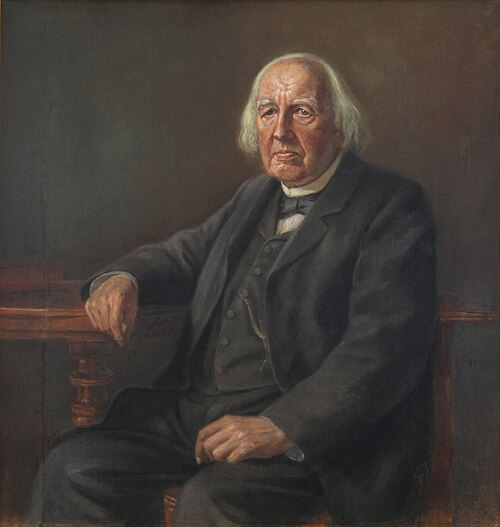
\includegraphics[width=\linewidth]{karl-weierstrass.jpg}\\
      {\scriptsize\color{gray}Portrait de Conrad Fehr (1895).
      Domaine public, Wikimedia Commons.}
    \end{column}
    \begin{column}{0.72\textwidth}
      \begin{itemize}
        \item Né en Westphalie ; envoyé étudier le droit à Bonn, il y
          passe quatre ans surtout à faire de l'escrime et à fréquenter
          les tavernes, et repart sans diplôme.
        \item Près de quinze ans enseignant au secondaire dans de petites
          villes de Prusse : mathématiques, physique, mais aussi
          allemand, botanique, géographie, gymnastique, calligraphie.
        \item Il poursuit ses recherches seul, le soir. Avant l'analyse,
          il a donc exercé le métier auquel vous vous préparez.
      \end{itemize}
    \end{column}
  \end{columns}
\end{frame}

\begin{frame}{Note historique 3.3 (suite)}
  \small
  \begin{itemize}
    \item 1854 : un article sur les fonctions abéliennes attire
      l'attention ; doctorat honorifique de Königsberg ; appelé à Berlin
      en 1856, à quarante ans.
    \item L'un des professeurs les plus influents de son siècle : la
      rigueur de l'analyse moderne, les définitions de limite et de
      continuité par $\varepsilon$ et $\delta$ --- celles du chapitre 2.
    \item Élèves : Cantor, Schwarz, Mittag-Leffler (directeur de thèse de
      von Koch), et Sofia Kovalevskaïa, à qui il donne des leçons privées
      pendant quatre ans, l'université refusant alors les femmes ; elle
      devient en 1889 l'une des premières professeures de mathématiques
      en Europe.
    \item Sa fonction de 1872 n'est publiée qu'en 1875, par Paul du
      Bois-Reymond.
  \end{itemize}
\end{frame}

\subsection{Mandelbrot et la géométrie de la nature}

\begin{frame}{Combien mesure la côte de la Grande-Bretagne ? (1967)}
  \small
  \begin{itemize}
    \item Richardson : la longueur mesurée d'une côte dépend de l'unité.
      Plus le compas est petit ($\varepsilon$), plus il épouse de baies,
      plus la longueur est grande :
      $L(\varepsilon)\approx C\,\varepsilon^{1-D}$, avec
      $D\approx\num{1.25}$ pour la côte ouest britannique.
    \item Mandelbrot y voit une dimension fractionnaire. Von Koch mesurée
      avec des segments de longueur $\big(\tfrac13\big)^n$ :
      $\big(\tfrac43\big)^n = \varepsilon^{1-D}$ avec $D=\ln4/\ln3$.
    \item Une côte est autosimilaire au sens statistique
      (remarque 3.2) ; sa dimension mesure son irrégularité.
    \item The Fractal Geometry of Nature (1982) : « Les nuages ne sont pas
      des sphères, les montagnes ne sont pas des cônes, les côtes ne sont
      pas des cercles, l'écorce n'est pas lisse, et l'éclair ne se propage
      pas en ligne droite. »
    \item L'ensemble de Mandelbrot ($z\mapsto z^2+c$) ne provient pas d'un
      SIF : hors du cadre de ce chapitre.
  \end{itemize}
\end{frame}

\begin{frame}{Note historique 3.4 --- Benoît Mandelbrot (1924--2010)}
  \footnotesize
  \begin{columns}[T]
    \begin{column}{0.25\textwidth}
      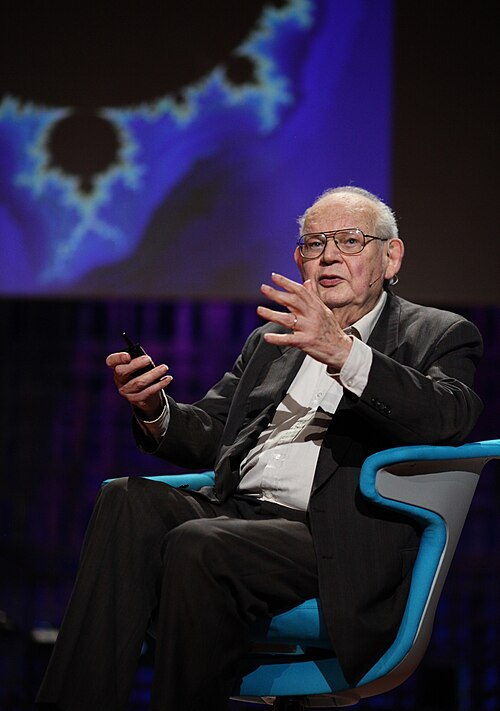
\includegraphics[width=\linewidth]{benoit-mandelbrot.jpg}\\
      {\scriptsize\color{gray}En 2010. Photo : Steve Jurvetson,
      CC BY 2.0, Wikimedia Commons.}
    \end{column}
    \begin{column}{0.72\textwidth}
      \begin{itemize}
        \item Né à Varsovie, famille juive d'origine lituanienne, émigrée
          en France en 1936 ; son oncle Szolem Mandelbrojt est professeur
          au Collège de France.
        \item Sous l'Occupation, la famille se cache ; scolarité
          interrompue. Faute de formation régulière, il développe une
          approche fondée sur la visualisation géométrique.
        \item Polytechnique (1944), aéronautique à Caltech, thèse à Paris
          (1952) sur la distribution statistique des mots.
      \end{itemize}
    \end{column}
  \end{columns}
\end{frame}

\begin{frame}{Note historique 3.4 (suite)}
  \small
  \begin{itemize}
    \item 1958 : choisit IBM, près de New York, plutôt qu'une université ;
      il y reste trente-cinq ans.
    \item Linguistique, économie, hydrologie, physique, astronomie : des
      déplacements entre disciplines qui suscitent la méfiance, mais lui
      font voir des structures communes.
    \item 1975 : forge le mot « fractal » (Les objets fractals : forme,
      hasard et dimension).
    \item Prix Wolf de physique (1993), prix du Japon (2003) ; professeur
      titulaire à Yale en 1999, à $75$ ans. Mort en 2010.
  \end{itemize}
\end{frame}

\subsection{Les fractales et la finance}

\begin{frame}{Le modèle classique, et ce que Mandelbrot observe}
  \small
  \begin{itemize}
    \item Bachelier (1900, Théorie de la spéculation) : le cours d'une
      action comme une marche au hasard, variations indépendantes et
      normales --- à la limite, le mouvement brownien. Fondement de la
      finance moderne (portefeuille, Black et Scholes, 1973).
    \item Mandelbrot (1963), prix du coton sur plusieurs décennies :
      \begin{enumerate}
        \item les grandes variations sont beaucoup trop fréquentes
          (« queues épaisses », lois stables de Lévy) : l'effet Noé ;
        \item la forme des variations ne dépend pas de l'échelle de
          temps : le graphe est statistiquement auto-affine ; sans les
          axes, impossible de dire s'il couvre un jour, un mois ou un an.
      \end{enumerate}
    \item Plus tard : périodes agitées et calmes se regroupent, une
      forme de mémoire --- l'effet Joseph.
  \end{itemize}
\end{frame}

\begin{frame}{Figure 3.16 --- Une « caricature » de cours boursier}
  \small Tendance de $(0,0)$ à $(1,1)$ ; générateur $(0,0)$,
  $\big(\tfrac49,\tfrac23\big)$, $\big(\tfrac59,\tfrac13\big)$, $(1,1)$.
  C'est l'attracteur du SIF
  \[
    w_1 = \mat{\tfrac49}{0}{0}{\tfrac23}\vec x,\quad
    w_2 = \mat{\tfrac19}{0}{0}{-\tfrac13}\vec x+\col{\tfrac49}{\tfrac23},\quad
    w_3 = \mat{\tfrac49}{0}{0}{\tfrac23}\vec x+\col{\tfrac59}{\tfrac13},
  \]
  avec $|\Delta y|=\sqrt{\Delta x}$ sur chaque morceau, comme le
  mouvement brownien.
  \FigBox[0.36\textheight]{%
    \begin{tikzpicture}[courbe/.style={sectioncolor, line join=round, thick}]
      \begin{scope}[scale=2.5]
        \draw[gray!50, dashed] (0,0) -- (1,1);
        % Cartoon de Mandelbrot, étape 1
% Fichier généré par generer.py : ne pas modifier à la main.
\draw[courbe]
  (0,0) -- (0.4444,0.6667) -- (0.5556,0.3333) -- (1,1);

        \foreach \p/\t/\pos in {(0,0)/{$(0,0)$}/right, (0.4444,0.6667)/{$(\frac49,\frac23)$}/left,
                              (0.5556,0.3333)/{$(\frac59,\frac13)$}/right, (1,1)/{$(1,1)$}/left}
          \node[pt, label={[etiq]\pos:\t}] at \p {};
        \node[etiq, sectioncolor] at (0.5,-0.18) {le générateur};
      \end{scope}
      \begin{scope}[shift={(3.4,0)}, scale=2.5]
        % Cartoon de Mandelbrot, étape 2
% Fichier généré par generer.py : ne pas modifier à la main.
\draw[courbe]
  (0,0) -- (0.1975,0.4444) -- (0.2469,0.2222) -- (0.4444,0.6667) -- (0.4938,0.4444) -- (0.5062,0.5556) --
  (0.5556,0.3333) -- (0.7531,0.7778) -- (0.8025,0.5556) -- (1,1);

        \node[etiq, sectioncolor] at (0.5,-0.18) {deuxième étape};
      \end{scope}
      \begin{scope}[shift={(6.8,0)}, scale=2.5, courbe/.style={sectioncolor, line join=round, very thin}]
        % Cartoon de Mandelbrot, étape 7
% Fichier généré par generer.py : ne pas modifier à la main.
\draw[courbe]
  (0,0) -- (0.0034,0.0585) -- (0.0043,0.0293) -- (0.0077,0.0878) -- (0.0086,0.0585) -- (0.0088,0.0732) --
  (0.0096,0.0439) -- (0.0131,0.1024) -- (0.0139,0.0732) -- (0.0173,0.1317) -- (0.0182,0.1024) -- (0.0184,0.1171) --
  (0.0193,0.0878) -- (0.0195,0.1024) -- (0.0195,0.0951) -- (0.0198,0.1097) -- (0.0206,0.0805) -- (0.0208,0.0951) --
  (0.0217,0.0658) -- (0.0251,0.1244) -- (0.026,0.0951) -- (0.0294,0.1536) -- (0.0302,0.1244) -- (0.0305,0.139) --
  (0.0313,0.1097) -- (0.0347,0.1683) -- (0.0356,0.139) -- (0.039,0.1975) -- (0.0399,0.1683) -- (0.0401,0.1829) --
  (0.0409,0.1536) -- (0.0412,0.1683) -- (0.0412,0.161) -- (0.0414,0.1756) -- (0.0423,0.1463) -- (0.0425,0.161) --
  (0.0434,0.1317) -- (0.0436,0.1463) -- (0.0436,0.139) -- (0.0438,0.1536) -- (0.0439,0.1463) -- (0.0439,0.15) --
  (0.044,0.1427) -- (0.0442,0.1573) -- (0.0442,0.15) -- (0.0444,0.1646) -- (0.0453,0.1353) -- (0.0455,0.15) --
  (0.0464,0.1207) -- (0.0466,0.1353) -- (0.0466,0.128) -- (0.0468,0.1427) -- (0.0477,0.1134) -- (0.0479,0.128) --
  (0.0488,0.0988) -- (0.0522,0.1573) -- (0.0531,0.128) -- (0.0565,0.1866) -- (0.0573,0.1573) -- (0.0576,0.1719) --
  (0.0584,0.1427) -- (0.0618,0.2012) -- (0.0627,0.1719) -- (0.0661,0.2305) -- (0.067,0.2012) -- (0.0672,0.2158) --
  (0.068,0.1866) -- (0.0683,0.2012) -- (0.0683,0.1939) -- (0.0685,0.2085) -- (0.0694,0.1792) -- (0.0696,0.1939) --
  (0.0704,0.1646) -- (0.0739,0.2231) -- (0.0747,0.1939) -- (0.0782,0.2524) -- (0.079,0.2231) -- (0.0792,0.2378) --
  (0.0801,0.2085) -- (0.0835,0.267) -- (0.0844,0.2378) -- (0.0878,0.2963) -- (0.0886,0.267) -- (0.0889,0.2817) --
  (0.0897,0.2524) -- (0.0899,0.267) -- (0.09,0.2597) -- (0.0902,0.2743) -- (0.0911,0.2451) -- (0.0913,0.2597) --
  (0.0921,0.2305) -- (0.0923,0.2451) -- (0.0924,0.2378) -- (0.0926,0.2524) -- (0.0927,0.2451) -- (0.0927,0.2487) --
  (0.0927,0.2414) -- (0.0929,0.2561) -- (0.093,0.2487) -- (0.0932,0.2634) -- (0.0941,0.2341) -- (0.0943,0.2487) --
  (0.0951,0.2195) -- (0.0954,0.2341) -- (0.0954,0.2268) -- (0.0956,0.2414) -- (0.0965,0.2122) -- (0.0967,0.2268) --
  (0.0975,0.1975) -- (0.0978,0.2122) -- (0.0978,0.2048) -- (0.098,0.2195) -- (0.0981,0.2122) -- (0.0981,0.2158) --
  (0.0981,0.2085) -- (0.0984,0.2231) -- (0.0984,0.2158) -- (0.0986,0.2305) -- (0.0987,0.2231) -- (0.0987,0.2268) --
  (0.0988,0.2195) -- (0.0988,0.2231) -- (0.0988,0.2213) -- (0.0988,0.225) -- (0.0988,0.2176) -- (0.0988,0.2213) --
  (0.0989,0.214) -- (0.0991,0.2286) -- (0.0992,0.2213) -- (0.0994,0.2359) -- (0.0994,0.2286) -- (0.0994,0.2323) --
  (0.0995,0.225) -- (0.0997,0.2396) -- (0.0998,0.2323) -- (0.1,0.2469) -- (0.1008,0.2176) -- (0.1011,0.2323) --
  (0.1019,0.203) -- (0.1021,0.2176) -- (0.1022,0.2103) -- (0.1024,0.225) -- (0.1032,0.1957) -- (0.1035,0.2103) --
  (0.1043,0.1811) -- (0.1045,0.1957) -- (0.1046,0.1884) -- (0.1048,0.203) -- (0.1049,0.1957) -- (0.1049,0.1994) --
  (0.1049,0.192) -- (0.1051,0.2067) -- (0.1052,0.1994) -- (0.1054,0.214) -- (0.1063,0.1847) -- (0.1065,0.1994) --
  (0.1073,0.1701) -- (0.1075,0.1847) -- (0.1076,0.1774) -- (0.1078,0.192) -- (0.1087,0.1628) -- (0.1089,0.1774) --
  (0.1097,0.1481) -- (0.1132,0.2067) -- (0.114,0.1774) -- (0.1174,0.2359) -- (0.1183,0.2067) -- (0.1185,0.2213) --
  (0.1194,0.192) -- (0.1228,0.2506) -- (0.1237,0.2213) -- (0.1271,0.2798) -- (0.1279,0.2506) -- (0.1282,0.2652) --
  (0.129,0.2359) -- (0.1292,0.2506) -- (0.1293,0.2433) -- (0.1295,0.2579) -- (0.1303,0.2286) -- (0.1306,0.2433) --
  (0.1314,0.214) -- (0.1348,0.2725) -- (0.1357,0.2433) -- (0.1391,0.3018) -- (0.14,0.2725) -- (0.1402,0.2872) --
  (0.1411,0.2579) -- (0.1445,0.3164) -- (0.1453,0.2872) -- (0.1488,0.3457) -- (0.1496,0.3164) -- (0.1498,0.331) --
  (0.1507,0.3018) -- (0.1509,0.3164) -- (0.151,0.3091) -- (0.1512,0.3237) -- (0.152,0.2945) -- (0.1522,0.3091) --
  (0.1531,0.2798) -- (0.1533,0.2945) -- (0.1534,0.2872) -- (0.1536,0.3018) -- (0.1536,0.2945) -- (0.1536,0.2981) --
  (0.1537,0.2908) -- (0.1539,0.3054) -- (0.154,0.2981) -- (0.1542,0.3128) -- (0.155,0.2835) -- (0.1552,0.2981) --
  (0.1561,0.2689) -- (0.1563,0.2835) -- (0.1564,0.2762) -- (0.1566,0.2908) -- (0.1574,0.2615) -- (0.1577,0.2762) --
  (0.1585,0.2469) -- (0.1619,0.3054) -- (0.1628,0.2762) -- (0.1662,0.3347) -- (0.1671,0.3054) -- (0.1673,0.3201) --
  (0.1681,0.2908) -- (0.1716,0.3493) -- (0.1724,0.3201) -- (0.1759,0.3786) -- (0.1767,0.3493) -- (0.1769,0.364) --
  (0.1778,0.3347) -- (0.178,0.3493) -- (0.178,0.342) -- (0.1783,0.3567) -- (0.1791,0.3274) -- (0.1793,0.342) --
  (0.1802,0.3128) -- (0.1836,0.3713) -- (0.1845,0.342) -- (0.1879,0.4005) -- (0.1888,0.3713) -- (0.189,0.3859) --
  (0.1898,0.3567) -- (0.1932,0.4152) -- (0.1941,0.3859) -- (0.1975,0.4444) -- (0.1984,0.4152) -- (0.1986,0.4298) --
  (0.1995,0.4005) -- (0.1997,0.4152) -- (0.1997,0.4079) -- (0.1999,0.4225) -- (0.2008,0.3932) -- (0.201,0.4079) --
  (0.2019,0.3786) -- (0.2021,0.3932) -- (0.2021,0.3859) -- (0.2023,0.4005) -- (0.2024,0.3932) -- (0.2024,0.3969) --
  (0.2025,0.3896) -- (0.2027,0.4042) -- (0.2027,0.3969) -- (0.203,0.4115) -- (0.2038,0.3823) -- (0.204,0.3969) --
  (0.2049,0.3676) -- (0.2051,0.3823) -- (0.2051,0.3749) -- (0.2054,0.3896) -- (0.2062,0.3603) -- (0.2064,0.3749) --
  (0.2073,0.3457) -- (0.2075,0.3603) -- (0.2076,0.353) -- (0.2078,0.3676) -- (0.2078,0.3603) -- (0.2078,0.364) --
  (0.2079,0.3567) -- (0.2081,0.3713) -- (0.2082,0.364) -- (0.2084,0.3786) -- (0.2084,0.3713) -- (0.2084,0.3749) --
  (0.2085,0.3676) -- (0.2085,0.3713) -- (0.2085,0.3695) -- (0.2085,0.3731) -- (0.2086,0.3658) -- (0.2086,0.3695) --
  (0.2086,0.3621) -- (0.2089,0.3768) -- (0.2089,0.3695) -- (0.2091,0.3841) -- (0.2092,0.3768) -- (0.2092,0.3804) --
  (0.2092,0.3731) -- (0.2095,0.3877) -- (0.2095,0.3804) -- (0.2097,0.3951) -- (0.2106,0.3658) -- (0.2108,0.3804) --
  (0.2117,0.3512) -- (0.2119,0.3658) -- (0.2119,0.3585) -- (0.2121,0.3731) -- (0.213,0.3439) -- (0.2132,0.3585) --
  (0.2141,0.3292) -- (0.2143,0.3439) -- (0.2143,0.3365) -- (0.2145,0.3512) -- (0.2146,0.3439) -- (0.2146,0.3475) --
  (0.2147,0.3402) -- (0.2149,0.3548) -- (0.2149,0.3475) -- (0.2151,0.3621) -- (0.216,0.3329) -- (0.2162,0.3475) --
  (0.2171,0.3182) -- (0.2173,0.3329) -- (0.2173,0.3256) -- (0.2176,0.3402) -- (0.2184,0.3109) -- (0.2186,0.3256) --
  (0.2195,0.2963) -- (0.2197,0.3109) -- (0.2197,0.3036) -- (0.22,0.3182) -- (0.22,0.3109) -- (0.22,0.3146) --
  (0.2201,0.3073) -- (0.2203,0.3219) -- (0.2203,0.3146) -- (0.2206,0.3292) -- (0.2206,0.3219) -- (0.2206,0.3256) --
  (0.2207,0.3182) -- (0.2207,0.3219) -- (0.2207,0.3201) -- (0.2207,0.3237) -- (0.2208,0.3164) -- (0.2208,0.3201) --
  (0.2208,0.3128) -- (0.221,0.3274) -- (0.2211,0.3201) -- (0.2213,0.3347) -- (0.2214,0.3274) -- (0.2214,0.331) --
  (0.2214,0.3237) -- (0.2216,0.3384) -- (0.2217,0.331) -- (0.2219,0.3457) -- (0.222,0.3384) -- (0.222,0.342) --
  (0.222,0.3347) -- (0.2221,0.3384) -- (0.2221,0.3365) -- (0.2221,0.3402) -- (0.2221,0.3329) -- (0.2221,0.3365) --
  (0.2222,0.3292) -- (0.2222,0.3329) -- (0.2222,0.331) -- (0.2222,0.3347) -- (0.2222,0.3329) -- (0.2222,0.3338) --
  (0.2222,0.332) -- (0.2222,0.3356) -- (0.2222,0.3338) -- (0.2223,0.3374) -- (0.2223,0.3301) -- (0.2223,0.3338) --
  (0.2224,0.3265) -- (0.2224,0.3301) -- (0.2224,0.3283) -- (0.2224,0.332) -- (0.2225,0.3246) -- (0.2225,0.3283) --
  (0.2225,0.321) -- (0.2227,0.3356) -- (0.2228,0.3283) -- (0.223,0.3429) -- (0.2231,0.3356) -- (0.2231,0.3393) --
  (0.2231,0.332) -- (0.2233,0.3466) -- (0.2234,0.3393) -- (0.2236,0.3539) -- (0.2237,0.3466) -- (0.2237,0.3503) --
  (0.2237,0.3429) -- (0.2237,0.3466) -- (0.2237,0.3448) -- (0.2238,0.3484) -- (0.2238,0.3411) -- (0.2238,0.3448) --
  (0.2239,0.3374) -- (0.2241,0.3521) -- (0.2241,0.3448) -- (0.2244,0.3594) -- (0.2244,0.3521) -- (0.2244,0.3557) --
  (0.2245,0.3484) -- (0.2247,0.3631) -- (0.2248,0.3557) -- (0.225,0.3704) -- (0.2258,0.3411) -- (0.226,0.3557) --
  (0.2269,0.3265) -- (0.2271,0.3411) -- (0.2272,0.3338) -- (0.2274,0.3484) -- (0.2282,0.3192) -- (0.2284,0.3338) --
  (0.2293,0.3045) -- (0.2295,0.3192) -- (0.2296,0.3118) -- (0.2298,0.3265) -- (0.2298,0.3192) -- (0.2298,0.3228) --
  (0.2299,0.3155) -- (0.2301,0.3301) -- (0.2302,0.3228) -- (0.2304,0.3374) -- (0.2312,0.3082) -- (0.2315,0.3228) --
  (0.2323,0.2936) -- (0.2325,0.3082) -- (0.2326,0.3009) -- (0.2328,0.3155) -- (0.2336,0.2862) -- (0.2339,0.3009) --
  (0.2347,0.2716) -- (0.2349,0.2862) -- (0.235,0.2789) -- (0.2352,0.2936) -- (0.2353,0.2862) -- (0.2353,0.2899) --
  (0.2353,0.2826) -- (0.2355,0.2972) -- (0.2356,0.2899) -- (0.2358,0.3045) -- (0.2359,0.2972) -- (0.2359,0.3009) --
  (0.2359,0.2936) -- (0.2359,0.2972) -- (0.2359,0.2954) -- (0.236,0.299) -- (0.236,0.2917) -- (0.236,0.2954) --
  (0.2361,0.2881) -- (0.2363,0.3027) -- (0.2363,0.2954) -- (0.2366,0.31) -- (0.2366,0.3027) -- (0.2366,0.3064) --
  (0.2367,0.299) -- (0.2369,0.3137) -- (0.2369,0.3064) -- (0.2372,0.321) -- (0.238,0.2917) -- (0.2382,0.3064) --
  (0.2391,0.2771) -- (0.2393,0.2917) -- (0.2394,0.2844) -- (0.2396,0.299) -- (0.2404,0.2698) -- (0.2406,0.2844) --
  (0.2415,0.2551) -- (0.2417,0.2698) -- (0.2418,0.2625) -- (0.242,0.2771) -- (0.242,0.2698) -- (0.242,0.2734) --
  (0.2421,0.2661) -- (0.2423,0.2807) -- (0.2424,0.2734) -- (0.2426,0.2881) -- (0.2434,0.2588) -- (0.2436,0.2734) --
  (0.2445,0.2442) -- (0.2447,0.2588) -- (0.2448,0.2515) -- (0.245,0.2661) -- (0.2458,0.2369) -- (0.2461,0.2515) --
  (0.2469,0.2222) -- (0.2503,0.2807) -- (0.2512,0.2515) -- (0.2546,0.31) -- (0.2555,0.2807) -- (0.2557,0.2954) --
  (0.2565,0.2661) -- (0.26,0.3246) -- (0.2608,0.2954) -- (0.2643,0.3539) -- (0.2651,0.3246) -- (0.2653,0.3393) --
  (0.2662,0.31) -- (0.2664,0.3246) -- (0.2664,0.3173) -- (0.2667,0.332) -- (0.2675,0.3027) -- (0.2677,0.3173) --
  (0.2686,0.2881) -- (0.272,0.3466) -- (0.2729,0.3173) -- (0.2763,0.3759) -- (0.2772,0.3466) -- (0.2774,0.3612) --
  (0.2782,0.332) -- (0.2817,0.3905) -- (0.2825,0.3612) -- (0.2859,0.4198) -- (0.2868,0.3905) -- (0.287,0.4051) --
  (0.2879,0.3759) -- (0.2881,0.3905) -- (0.2881,0.3832) -- (0.2883,0.3978) -- (0.2892,0.3685) -- (0.2894,0.3832) --
  (0.2903,0.3539) -- (0.2905,0.3685) -- (0.2905,0.3612) -- (0.2907,0.3759) -- (0.2908,0.3685) -- (0.2908,0.3722) --
  (0.2909,0.3649) -- (0.2911,0.3795) -- (0.2911,0.3722) -- (0.2914,0.3868) -- (0.2922,0.3576) -- (0.2924,0.3722) --
  (0.2933,0.3429) -- (0.2935,0.3576) -- (0.2935,0.3503) -- (0.2938,0.3649) -- (0.2946,0.3356) -- (0.2948,0.3503) --
  (0.2957,0.321) -- (0.2991,0.3795) -- (0.3,0.3503) -- (0.3034,0.4088) -- (0.3043,0.3795) -- (0.3045,0.3941) --
  (0.3053,0.3649) -- (0.3087,0.4234) -- (0.3096,0.3941) -- (0.313,0.4527) -- (0.3139,0.4234) -- (0.3141,0.438) --
  (0.315,0.4088) -- (0.3152,0.4234) -- (0.3152,0.4161) -- (0.3154,0.4307) -- (0.3163,0.4015) -- (0.3165,0.4161) --
  (0.3174,0.3868) -- (0.3208,0.4454) -- (0.3216,0.4161) -- (0.3251,0.4746) -- (0.3259,0.4454) -- (0.3261,0.46) --
  (0.327,0.4307) -- (0.3304,0.4893) -- (0.3313,0.46) -- (0.3347,0.5185) -- (0.3356,0.4893) -- (0.3358,0.5039) --
  (0.3366,0.4746) -- (0.3368,0.4893) -- (0.3369,0.4819) -- (0.3371,0.4966) -- (0.338,0.4673) -- (0.3382,0.4819) --
  (0.339,0.4527) -- (0.3393,0.4673) -- (0.3393,0.46) -- (0.3395,0.4746) -- (0.3396,0.4673) -- (0.3396,0.471) --
  (0.3396,0.4636) -- (0.3399,0.4783) -- (0.3399,0.471) -- (0.3401,0.4856) -- (0.341,0.4563) -- (0.3412,0.471) --
  (0.3421,0.4417) -- (0.3423,0.4563) -- (0.3423,0.449) -- (0.3425,0.4636) -- (0.3434,0.4344) -- (0.3436,0.449) --
  (0.3445,0.4198) -- (0.3447,0.4344) -- (0.3447,0.4271) -- (0.3449,0.4417) -- (0.345,0.4344) -- (0.345,0.438) --
  (0.3451,0.4307) -- (0.3453,0.4454) -- (0.3453,0.438) -- (0.3455,0.4527) -- (0.3456,0.4454) -- (0.3456,0.449) --
  (0.3457,0.4417) -- (0.3457,0.4454) -- (0.3457,0.4435) -- (0.3457,0.4472) -- (0.3457,0.4399) -- (0.3458,0.4435) --
  (0.3458,0.4362) -- (0.346,0.4508) -- (0.3461,0.4435) -- (0.3463,0.4582) -- (0.3463,0.4508) -- (0.3464,0.4545) --
  (0.3464,0.4472) -- (0.3466,0.4618) -- (0.3467,0.4545) -- (0.3469,0.4691) -- (0.3478,0.4399) -- (0.348,0.4545) --
  (0.3488,0.4252) -- (0.349,0.4399) -- (0.3491,0.4326) -- (0.3493,0.4472) -- (0.3502,0.4179) -- (0.3504,0.4326) --
  (0.3512,0.4033) -- (0.3514,0.4179) -- (0.3515,0.4106) -- (0.3517,0.4252) -- (0.3518,0.4179) -- (0.3518,0.4216) --
  (0.3518,0.4143) -- (0.352,0.4289) -- (0.3521,0.4216) -- (0.3523,0.4362) -- (0.3532,0.407) -- (0.3534,0.4216) --
  (0.3542,0.3923) -- (0.3545,0.407) -- (0.3545,0.3996) -- (0.3547,0.4143) -- (0.3556,0.385) -- (0.3558,0.3996) --
  (0.3567,0.3704) -- (0.3601,0.4289) -- (0.3609,0.3996) -- (0.3644,0.4582) -- (0.3652,0.4289) -- (0.3654,0.4435) --
  (0.3663,0.4143) -- (0.3697,0.4728) -- (0.3706,0.4435) -- (0.374,0.5021) -- (0.3749,0.4728) -- (0.3751,0.4874) --
  (0.3759,0.4582) -- (0.3761,0.4728) -- (0.3762,0.4655) -- (0.3764,0.4801) -- (0.3773,0.4508) -- (0.3775,0.4655) --
  (0.3783,0.4362) -- (0.3818,0.4947) -- (0.3826,0.4655) -- (0.386,0.524) -- (0.3869,0.4947) -- (0.3871,0.5094) --
  (0.388,0.4801) -- (0.3914,0.5386) -- (0.3922,0.5094) -- (0.3957,0.5679) -- (0.3965,0.5386) -- (0.3967,0.5533) --
  (0.3976,0.524) -- (0.3978,0.5386) -- (0.3979,0.5313) -- (0.3981,0.546) -- (0.3989,0.5167) -- (0.3992,0.5313) --
  (0.4,0.5021) -- (0.4002,0.5167) -- (0.4003,0.5094) -- (0.4005,0.524) -- (0.4005,0.5167) -- (0.4006,0.5203) --
  (0.4006,0.513) -- (0.4008,0.5277) -- (0.4009,0.5203) -- (0.4011,0.535) -- (0.4019,0.5057) -- (0.4022,0.5203) --
  (0.403,0.4911) -- (0.4032,0.5057) -- (0.4033,0.4984) -- (0.4035,0.513) -- (0.4044,0.4838) -- (0.4046,0.4984) --
  (0.4054,0.4691) -- (0.4089,0.5277) -- (0.4097,0.4984) -- (0.4131,0.5569) -- (0.414,0.5277) -- (0.4142,0.5423) --
  (0.4151,0.513) -- (0.4185,0.5716) -- (0.4193,0.5423) -- (0.4228,0.6008) -- (0.4236,0.5716) -- (0.4238,0.5862) --
  (0.4247,0.5569) -- (0.4249,0.5716) -- (0.425,0.5642) -- (0.4252,0.5789) -- (0.426,0.5496) -- (0.4262,0.5642) --
  (0.4271,0.535) -- (0.4305,0.5935) -- (0.4314,0.5642) -- (0.4348,0.6228) -- (0.4357,0.5935) -- (0.4359,0.6081) --
  (0.4367,0.5789) -- (0.4402,0.6374) -- (0.441,0.6081) -- (0.4444,0.6667) -- (0.4453,0.6374) -- (0.4455,0.652) --
  (0.4464,0.6228) -- (0.4466,0.6374) -- (0.4466,0.6301) -- (0.4469,0.6447) -- (0.4477,0.6155) -- (0.4479,0.6301) --
  (0.4488,0.6008) -- (0.449,0.6155) -- (0.449,0.6081) -- (0.4493,0.6228) -- (0.4493,0.6155) -- (0.4493,0.6191) --
  (0.4494,0.6118) -- (0.4496,0.6264) -- (0.4496,0.6191) -- (0.4499,0.6337) -- (0.4507,0.6045) -- (0.4509,0.6191) --
  (0.4518,0.5898) -- (0.452,0.6045) -- (0.4521,0.5972) -- (0.4523,0.6118) -- (0.4531,0.5825) -- (0.4533,0.5972) --
  (0.4542,0.5679) -- (0.4544,0.5825) -- (0.4545,0.5752) -- (0.4547,0.5898) -- (0.4547,0.5825) -- (0.4547,0.5862) --
  (0.4548,0.5789) -- (0.455,0.5935) -- (0.4551,0.5862) -- (0.4553,0.6008) -- (0.4553,0.5935) -- (0.4553,0.5972) --
  (0.4554,0.5898) -- (0.4554,0.5935) -- (0.4554,0.5917) -- (0.4554,0.5953) -- (0.4555,0.588) -- (0.4555,0.5917) --
  (0.4556,0.5844) -- (0.4558,0.599) -- (0.4558,0.5917) -- (0.456,0.6063) -- (0.4561,0.599) -- (0.4561,0.6027) --
  (0.4562,0.5953) -- (0.4564,0.61) -- (0.4564,0.6027) -- (0.4566,0.6173) -- (0.4575,0.588) -- (0.4577,0.6027) --
  (0.4586,0.5734) -- (0.4588,0.588) -- (0.4588,0.5807) -- (0.459,0.5953) -- (0.4599,0.5661) -- (0.4601,0.5807) --
  (0.461,0.5514) -- (0.4612,0.5661) -- (0.4612,0.5588) -- (0.4615,0.5734) -- (0.4615,0.5661) -- (0.4615,0.5697) --
  (0.4616,0.5624) -- (0.4618,0.577) -- (0.4618,0.5697) -- (0.4621,0.5844) -- (0.4629,0.5551) -- (0.4631,0.5697) --
  (0.464,0.5405) -- (0.4642,0.5551) -- (0.4643,0.5478) -- (0.4645,0.5624) -- (0.4653,0.5332) -- (0.4655,0.5478) --
  (0.4664,0.5185) -- (0.4666,0.5332) -- (0.4667,0.5258) -- (0.4669,0.5405) -- (0.4669,0.5332) -- (0.4669,0.5368) --
  (0.467,0.5295) -- (0.4672,0.5441) -- (0.4673,0.5368) -- (0.4675,0.5514) -- (0.4675,0.5441) -- (0.4675,0.5478) --
  (0.4676,0.5405) -- (0.4676,0.5441) -- (0.4676,0.5423) -- (0.4676,0.546) -- (0.4677,0.5386) -- (0.4677,0.5423) --
  (0.4677,0.535) -- (0.468,0.5496) -- (0.468,0.5423) -- (0.4682,0.5569) -- (0.4683,0.5496) -- (0.4683,0.5533) --
  (0.4683,0.546) -- (0.4686,0.5606) -- (0.4686,0.5533) -- (0.4688,0.5679) -- (0.4689,0.5606) -- (0.4689,0.5642) --
  (0.469,0.5569) -- (0.469,0.5606) -- (0.469,0.5588) -- (0.469,0.5624) -- (0.469,0.5551) -- (0.469,0.5588) --
  (0.4691,0.5514) -- (0.4691,0.5551) -- (0.4691,0.5533) -- (0.4691,0.5569) -- (0.4691,0.5551) -- (0.4691,0.556) --
  (0.4691,0.5542) -- (0.4692,0.5578) -- (0.4692,0.556) -- (0.4692,0.5597) -- (0.4692,0.5524) -- (0.4692,0.556) --
  (0.4693,0.5487) -- (0.4693,0.5524) -- (0.4693,0.5505) -- (0.4693,0.5542) -- (0.4694,0.5469) -- (0.4694,0.5505) --
  (0.4694,0.5432) -- (0.4697,0.5578) -- (0.4697,0.5505) -- (0.4699,0.5652) -- (0.47,0.5578) -- (0.47,0.5615) --
  (0.47,0.5542) -- (0.4703,0.5688) -- (0.4703,0.5615) -- (0.4705,0.5761) -- (0.4706,0.5688) -- (0.4706,0.5725) --
  (0.4706,0.5652) -- (0.4707,0.5688) -- (0.4707,0.567) -- (0.4707,0.5706) -- (0.4707,0.5633) -- (0.4707,0.567) --
  (0.4708,0.5597) -- (0.471,0.5743) -- (0.4711,0.567) -- (0.4713,0.5816) -- (0.4713,0.5743) -- (0.4713,0.578) --
  (0.4714,0.5706) -- (0.4716,0.5853) -- (0.4717,0.578) -- (0.4719,0.5926) -- (0.4727,0.5633) -- (0.4729,0.578) --
  (0.4738,0.5487) -- (0.474,0.5633) -- (0.4741,0.556) -- (0.4743,0.5706) -- (0.4751,0.5414) -- (0.4754,0.556) --
  (0.4762,0.5267) -- (0.4764,0.5414) -- (0.4765,0.5341) -- (0.4767,0.5487) -- (0.4767,0.5414) -- (0.4768,0.545) --
  (0.4768,0.5377) -- (0.477,0.5524) -- (0.4771,0.545) -- (0.4773,0.5597) -- (0.4782,0.5304) -- (0.4784,0.545) --
  (0.4792,0.5158) -- (0.4794,0.5304) -- (0.4795,0.5231) -- (0.4797,0.5377) -- (0.4806,0.5085) -- (0.4808,0.5231) --
  (0.4816,0.4938) -- (0.4818,0.5085) -- (0.4819,0.5011) -- (0.4821,0.5158) -- (0.4822,0.5085) -- (0.4822,0.5121) --
  (0.4822,0.5048) -- (0.4825,0.5194) -- (0.4825,0.5121) -- (0.4827,0.5267) -- (0.4828,0.5194) -- (0.4828,0.5231) --
  (0.4828,0.5158) -- (0.4829,0.5194) -- (0.4829,0.5176) -- (0.4829,0.5213) -- (0.4829,0.5139) -- (0.4829,0.5176) --
  (0.483,0.5103) -- (0.4832,0.5249) -- (0.4833,0.5176) -- (0.4835,0.5322) -- (0.4835,0.5249) -- (0.4835,0.5286) --
  (0.4836,0.5213) -- (0.4838,0.5359) -- (0.4839,0.5286) -- (0.4841,0.5432) -- (0.4849,0.5139) -- (0.4851,0.5286) --
  (0.486,0.4993) -- (0.4862,0.5139) -- (0.4863,0.5066) -- (0.4865,0.5213) -- (0.4873,0.492) -- (0.4876,0.5066) --
  (0.4884,0.4774) -- (0.4886,0.492) -- (0.4887,0.4847) -- (0.4889,0.4993) -- (0.4889,0.492) -- (0.489,0.4957) --
  (0.489,0.4883) -- (0.4892,0.503) -- (0.4893,0.4957) -- (0.4895,0.5103) -- (0.4903,0.481) -- (0.4906,0.4957) --
  (0.4914,0.4664) -- (0.4916,0.481) -- (0.4917,0.4737) -- (0.4919,0.4883) -- (0.4928,0.4591) -- (0.493,0.4737) --
  (0.4938,0.4444) -- (0.494,0.4591) -- (0.4941,0.4518) -- (0.4943,0.4664) -- (0.4944,0.4591) -- (0.4944,0.4627) --
  (0.4944,0.4554) -- (0.4946,0.4701) -- (0.4947,0.4627) -- (0.4949,0.4774) -- (0.495,0.4701) -- (0.495,0.4737) --
  (0.495,0.4664) -- (0.495,0.4701) -- (0.495,0.4682) -- (0.4951,0.4719) -- (0.4951,0.4646) -- (0.4951,0.4682) --
  (0.4952,0.4609) -- (0.4954,0.4755) -- (0.4954,0.4682) -- (0.4957,0.4829) -- (0.4957,0.4755) -- (0.4957,0.4792) --
  (0.4958,0.4719) -- (0.496,0.4865) -- (0.4961,0.4792) -- (0.4963,0.4938) -- (0.4963,0.4865) -- (0.4963,0.4902) --
  (0.4964,0.4829) -- (0.4964,0.4865) -- (0.4964,0.4847) -- (0.4964,0.4883) -- (0.4965,0.481) -- (0.4965,0.4847) --
  (0.4965,0.4774) -- (0.4966,0.481) -- (0.4966,0.4792) -- (0.4966,0.4829) -- (0.4966,0.481) -- (0.4966,0.4819) --
  (0.4966,0.4801) -- (0.4966,0.4838) -- (0.4966,0.4819) -- (0.4966,0.4856) -- (0.4967,0.4783) -- (0.4967,0.4819) --
  (0.4967,0.4746) -- (0.4967,0.4783) -- (0.4967,0.4765) -- (0.4968,0.4801) -- (0.4968,0.4728) -- (0.4968,0.4765) --
  (0.4969,0.4691) -- (0.4971,0.4838) -- (0.4971,0.4765) -- (0.4974,0.4911) -- (0.4974,0.4838) -- (0.4974,0.4874) --
  (0.4975,0.4801) -- (0.4977,0.4947) -- (0.4977,0.4874) -- (0.498,0.5021) -- (0.498,0.4947) -- (0.498,0.4984) --
  (0.4981,0.4911) -- (0.4981,0.4947) -- (0.4981,0.4929) -- (0.4981,0.4966) -- (0.4982,0.4893) -- (0.4982,0.4929) --
  (0.4982,0.4856) -- (0.4984,0.5002) -- (0.4985,0.4929) -- (0.4987,0.5075) -- (0.4988,0.5002) -- (0.4988,0.5039) --
  (0.4988,0.4966) -- (0.499,0.5112) -- (0.4991,0.5039) -- (0.4993,0.5185) -- (0.4994,0.5112) -- (0.4994,0.5149) --
  (0.4994,0.5075) -- (0.4994,0.5112) -- (0.4995,0.5094) -- (0.4995,0.513) -- (0.4995,0.5057) -- (0.4995,0.5094) --
  (0.4996,0.5021) -- (0.4996,0.5057) -- (0.4996,0.5039) -- (0.4996,0.5075) -- (0.4996,0.5057) -- (0.4996,0.5066) --
  (0.4996,0.5048) -- (0.4996,0.5085) -- (0.4996,0.5066) -- (0.4997,0.5103) -- (0.4997,0.503) -- (0.4997,0.5066) --
  (0.4998,0.4993) -- (0.4998,0.503) -- (0.4998,0.5011) -- (0.4998,0.5048) -- (0.4999,0.4975) -- (0.4999,0.5011) --
  (0.4999,0.4938) -- (0.4999,0.4975) -- (0.4999,0.4957) -- (0.5,0.4993) -- (0.5,0.4975) -- (0.5,0.4984) --
  (0.5,0.4966) -- (0.5,0.5002) -- (0.5,0.4984) -- (0.5,0.5021) -- (0.5,0.5002) -- (0.5,0.5011) --
  (0.5,0.4993) -- (0.5,0.5002) -- (0.5,0.4998) -- (0.5,0.5007) -- (0.5,0.4989) -- (0.5,0.4998) --
  (0.5,0.4979) -- (0.5,0.5016) -- (0.5,0.4998) -- (0.5,0.5034) -- (0.5,0.5016) -- (0.5,0.5025) --
  (0.5,0.5007) -- (0.5001,0.5043) -- (0.5001,0.5025) -- (0.5001,0.5062) -- (0.5001,0.4989) -- (0.5001,0.5025) --
  (0.5002,0.4952) -- (0.5002,0.4989) -- (0.5002,0.497) -- (0.5002,0.5007) -- (0.5003,0.4934) -- (0.5003,0.497) --
  (0.5003,0.4897) -- (0.5004,0.4934) -- (0.5004,0.4915) -- (0.5004,0.4952) -- (0.5004,0.4934) -- (0.5004,0.4943) --
  (0.5004,0.4925) -- (0.5004,0.4961) -- (0.5004,0.4943) -- (0.5004,0.4979) -- (0.5005,0.4906) -- (0.5005,0.4943) --
  (0.5005,0.487) -- (0.5005,0.4906) -- (0.5006,0.4888) -- (0.5006,0.4925) -- (0.5006,0.4851) -- (0.5006,0.4888) --
  (0.5007,0.4815) -- (0.5009,0.4961) -- (0.501,0.4888) -- (0.5012,0.5034) -- (0.5012,0.4961) -- (0.5012,0.4998) --
  (0.5013,0.4925) -- (0.5015,0.5071) -- (0.5016,0.4998) -- (0.5018,0.5144) -- (0.5018,0.5071) -- (0.5018,0.5107) --
  (0.5019,0.5034) -- (0.5019,0.5071) -- (0.5019,0.5053) -- (0.5019,0.5089) -- (0.502,0.5016) -- (0.502,0.5053) --
  (0.502,0.4979) -- (0.5023,0.5126) -- (0.5023,0.5053) -- (0.5025,0.5199) -- (0.5026,0.5126) -- (0.5026,0.5162) --
  (0.5026,0.5089) -- (0.5029,0.5235) -- (0.5029,0.5162) -- (0.5031,0.5309) -- (0.5032,0.5235) -- (0.5032,0.5272) --
  (0.5032,0.5199) -- (0.5033,0.5235) -- (0.5033,0.5217) -- (0.5033,0.5254) -- (0.5033,0.5181) -- (0.5033,0.5217) --
  (0.5034,0.5144) -- (0.5034,0.5181) -- (0.5034,0.5162) -- (0.5034,0.5199) -- (0.5034,0.5181) -- (0.5034,0.519) --
  (0.5034,0.5171) -- (0.5034,0.5208) -- (0.5034,0.519) -- (0.5035,0.5226) -- (0.5035,0.5153) -- (0.5035,0.519) --
  (0.5036,0.5117) -- (0.5036,0.5153) -- (0.5036,0.5135) -- (0.5036,0.5171) -- (0.5037,0.5098) -- (0.5037,0.5135) --
  (0.5037,0.5062) -- (0.5039,0.5208) -- (0.504,0.5135) -- (0.5042,0.5281) -- (0.5043,0.5208) -- (0.5043,0.5245) --
  (0.5043,0.5171) -- (0.5046,0.5318) -- (0.5046,0.5245) -- (0.5048,0.5391) -- (0.5049,0.5318) -- (0.5049,0.5354) --
  (0.5049,0.5281) -- (0.505,0.5318) -- (0.505,0.5299) -- (0.505,0.5336) -- (0.505,0.5263) -- (0.505,0.5299) --
  (0.5051,0.5226) -- (0.5053,0.5373) -- (0.5054,0.5299) -- (0.5056,0.5446) -- (0.5056,0.5373) -- (0.5056,0.5409) --
  (0.5057,0.5336) -- (0.5059,0.5482) -- (0.506,0.5409) -- (0.5062,0.5556) -- (0.507,0.5263) -- (0.5072,0.5409) --
  (0.5081,0.5117) -- (0.5083,0.5263) -- (0.5084,0.519) -- (0.5086,0.5336) -- (0.5094,0.5043) -- (0.5097,0.519) --
  (0.5105,0.4897) -- (0.5107,0.5043) -- (0.5108,0.497) -- (0.511,0.5117) -- (0.511,0.5043) -- (0.5111,0.508) --
  (0.5111,0.5007) -- (0.5113,0.5153) -- (0.5114,0.508) -- (0.5116,0.5226) -- (0.5124,0.4934) -- (0.5127,0.508) --
  (0.5135,0.4787) -- (0.5137,0.4934) -- (0.5138,0.4861) -- (0.514,0.5007) -- (0.5149,0.4714) -- (0.5151,0.4861) --
  (0.5159,0.4568) -- (0.5161,0.4714) -- (0.5162,0.4641) -- (0.5164,0.4787) -- (0.5165,0.4714) -- (0.5165,0.4751) --
  (0.5165,0.4678) -- (0.5167,0.4824) -- (0.5168,0.4751) -- (0.517,0.4897) -- (0.5171,0.4824) -- (0.5171,0.4861) --
  (0.5171,0.4787) -- (0.5171,0.4824) -- (0.5171,0.4806) -- (0.5172,0.4842) -- (0.5172,0.4769) -- (0.5172,0.4806) --
  (0.5173,0.4733) -- (0.5175,0.4879) -- (0.5175,0.4806) -- (0.5178,0.4952) -- (0.5178,0.4879) -- (0.5178,0.4915) --
  (0.5179,0.4842) -- (0.5181,0.4989) -- (0.5182,0.4915) -- (0.5184,0.5062) -- (0.5192,0.4769) -- (0.5194,0.4915) --
  (0.5203,0.4623) -- (0.5205,0.4769) -- (0.5206,0.4696) -- (0.5208,0.4842) -- (0.5216,0.455) -- (0.5218,0.4696) --
  (0.5227,0.4403) -- (0.5229,0.455) -- (0.523,0.4476) -- (0.5232,0.4623) -- (0.5232,0.455) -- (0.5233,0.4586) --
  (0.5233,0.4513) -- (0.5235,0.4659) -- (0.5236,0.4586) -- (0.5238,0.4733) -- (0.5246,0.444) -- (0.5249,0.4586) --
  (0.5257,0.4294) -- (0.5259,0.444) -- (0.526,0.4367) -- (0.5262,0.4513) -- (0.5271,0.422) -- (0.5273,0.4367) --
  (0.5281,0.4074) -- (0.5283,0.422) -- (0.5284,0.4147) -- (0.5286,0.4294) -- (0.5287,0.422) -- (0.5287,0.4257) --
  (0.5287,0.4184) -- (0.5289,0.433) -- (0.529,0.4257) -- (0.5292,0.4403) -- (0.5293,0.433) -- (0.5293,0.4367) --
  (0.5293,0.4294) -- (0.5293,0.433) -- (0.5293,0.4312) -- (0.5294,0.4348) -- (0.5294,0.4275) -- (0.5294,0.4312) --
  (0.5295,0.4239) -- (0.5297,0.4385) -- (0.5297,0.4312) -- (0.53,0.4458) -- (0.53,0.4385) -- (0.53,0.4422) --
  (0.5301,0.4348) -- (0.5303,0.4495) -- (0.5303,0.4422) -- (0.5306,0.4568) -- (0.5306,0.4495) -- (0.5306,0.4531) --
  (0.5307,0.4458) -- (0.5307,0.4495) -- (0.5307,0.4476) -- (0.5307,0.4513) -- (0.5308,0.444) -- (0.5308,0.4476) --
  (0.5308,0.4403) -- (0.5308,0.444) -- (0.5308,0.4422) -- (0.5309,0.4458) -- (0.5309,0.444) -- (0.5309,0.4449) --
  (0.5309,0.4431) -- (0.5309,0.4467) -- (0.5309,0.4449) -- (0.5309,0.4486) -- (0.531,0.4412) -- (0.531,0.4449) --
  (0.531,0.4376) -- (0.531,0.4412) -- (0.531,0.4394) -- (0.531,0.4431) -- (0.5311,0.4358) -- (0.5311,0.4394) --
  (0.5312,0.4321) -- (0.5314,0.4467) -- (0.5314,0.4394) -- (0.5317,0.454) -- (0.5317,0.4467) -- (0.5317,0.4504) --
  (0.5318,0.4431) -- (0.532,0.4577) -- (0.532,0.4504) -- (0.5323,0.465) -- (0.5323,0.4577) -- (0.5323,0.4614) --
  (0.5324,0.454) -- (0.5324,0.4577) -- (0.5324,0.4559) -- (0.5324,0.4595) -- (0.5325,0.4522) -- (0.5325,0.4559) --
  (0.5325,0.4486) -- (0.5327,0.4632) -- (0.5328,0.4559) -- (0.533,0.4705) -- (0.5331,0.4632) -- (0.5331,0.4668) --
  (0.5331,0.4595) -- (0.5333,0.4742) -- (0.5334,0.4668) -- (0.5336,0.4815) -- (0.5345,0.4522) -- (0.5347,0.4668) --
  (0.5355,0.4376) -- (0.5357,0.4522) -- (0.5358,0.4449) -- (0.536,0.4595) -- (0.5369,0.4303) -- (0.5371,0.4449) --
  (0.5379,0.4156) -- (0.5382,0.4303) -- (0.5382,0.423) -- (0.5384,0.4376) -- (0.5385,0.4303) -- (0.5385,0.4339) --
  (0.5385,0.4266) -- (0.5388,0.4412) -- (0.5388,0.4339) -- (0.539,0.4486) -- (0.5399,0.4193) -- (0.5401,0.4339) --
  (0.541,0.4047) -- (0.5412,0.4193) -- (0.5412,0.412) -- (0.5414,0.4266) -- (0.5423,0.3973) -- (0.5425,0.412) --
  (0.5434,0.3827) -- (0.5436,0.3973) -- (0.5436,0.39) -- (0.5438,0.4047) -- (0.5439,0.3973) -- (0.5439,0.401) --
  (0.544,0.3937) -- (0.5442,0.4083) -- (0.5442,0.401) -- (0.5444,0.4156) -- (0.5445,0.4083) -- (0.5445,0.412) --
  (0.5446,0.4047) -- (0.5446,0.4083) -- (0.5446,0.4065) -- (0.5446,0.4102) -- (0.5447,0.4028) -- (0.5447,0.4065) --
  (0.5447,0.3992) -- (0.5449,0.4138) -- (0.545,0.4065) -- (0.5452,0.4211) -- (0.5453,0.4138) -- (0.5453,0.4175) --
  (0.5453,0.4102) -- (0.5455,0.4248) -- (0.5456,0.4175) -- (0.5458,0.4321) -- (0.5467,0.4028) -- (0.5469,0.4175) --
  (0.5477,0.3882) -- (0.5479,0.4028) -- (0.548,0.3955) -- (0.5482,0.4102) -- (0.5491,0.3809) -- (0.5493,0.3955) --
  (0.5501,0.3663) -- (0.5504,0.3809) -- (0.5504,0.3736) -- (0.5506,0.3882) -- (0.5507,0.3809) -- (0.5507,0.3845) --
  (0.5507,0.3772) -- (0.551,0.3919) -- (0.551,0.3845) -- (0.5512,0.3992) -- (0.5521,0.3699) -- (0.5523,0.3845) --
  (0.5531,0.3553) -- (0.5534,0.3699) -- (0.5534,0.3626) -- (0.5536,0.3772) -- (0.5545,0.348) -- (0.5547,0.3626) --
  (0.5556,0.3333) -- (0.559,0.3919) -- (0.5598,0.3626) -- (0.5633,0.4211) -- (0.5641,0.3919) -- (0.5643,0.4065) --
  (0.5652,0.3772) -- (0.5686,0.4358) -- (0.5695,0.4065) -- (0.5729,0.465) -- (0.5738,0.4358) -- (0.574,0.4504) --
  (0.5748,0.4211) -- (0.575,0.4358) -- (0.5751,0.4284) -- (0.5753,0.4431) -- (0.5762,0.4138) -- (0.5764,0.4284) --
  (0.5772,0.3992) -- (0.5807,0.4577) -- (0.5815,0.4284) -- (0.5849,0.487) -- (0.5858,0.4577) -- (0.586,0.4723) --
  (0.5869,0.4431) -- (0.5903,0.5016) -- (0.5911,0.4723) -- (0.5946,0.5309) -- (0.5954,0.5016) -- (0.5956,0.5162) --
  (0.5965,0.487) -- (0.5967,0.5016) -- (0.5968,0.4943) -- (0.597,0.5089) -- (0.5978,0.4797) -- (0.5981,0.4943) --
  (0.5989,0.465) -- (0.5991,0.4797) -- (0.5992,0.4723) -- (0.5994,0.487) -- (0.5994,0.4797) -- (0.5995,0.4833) --
  (0.5995,0.476) -- (0.5997,0.4906) -- (0.5998,0.4833) -- (0.6,0.4979) -- (0.6008,0.4687) -- (0.6011,0.4833) --
  (0.6019,0.454) -- (0.6021,0.4687) -- (0.6022,0.4614) -- (0.6024,0.476) -- (0.6033,0.4467) -- (0.6035,0.4614) --
  (0.6043,0.4321) -- (0.6078,0.4906) -- (0.6086,0.4614) -- (0.612,0.5199) -- (0.6129,0.4906) -- (0.6131,0.5053) --
  (0.614,0.476) -- (0.6174,0.5345) -- (0.6182,0.5053) -- (0.6217,0.5638) -- (0.6225,0.5345) -- (0.6227,0.5492) --
  (0.6236,0.5199) -- (0.6238,0.5345) -- (0.6239,0.5272) -- (0.6241,0.5418) -- (0.6249,0.5126) -- (0.6251,0.5272) --
  (0.626,0.4979) -- (0.6294,0.5565) -- (0.6303,0.5272) -- (0.6337,0.5857) -- (0.6346,0.5565) -- (0.6348,0.5711) --
  (0.6356,0.5418) -- (0.6391,0.6004) -- (0.6399,0.5711) -- (0.6433,0.6296) -- (0.6442,0.6004) -- (0.6444,0.615) --
  (0.6453,0.5857) -- (0.6455,0.6004) -- (0.6455,0.593) -- (0.6458,0.6077) -- (0.6466,0.5784) -- (0.6468,0.593) --
  (0.6477,0.5638) -- (0.6479,0.5784) -- (0.648,0.5711) -- (0.6482,0.5857) -- (0.6482,0.5784) -- (0.6482,0.5821) --
  (0.6483,0.5748) -- (0.6485,0.5894) -- (0.6486,0.5821) -- (0.6488,0.5967) -- (0.6496,0.5674) -- (0.6498,0.5821) --
  (0.6507,0.5528) -- (0.6509,0.5674) -- (0.651,0.5601) -- (0.6512,0.5748) -- (0.652,0.5455) -- (0.6522,0.5601) --
  (0.6531,0.5309) -- (0.6533,0.5455) -- (0.6534,0.5382) -- (0.6536,0.5528) -- (0.6536,0.5455) -- (0.6537,0.5492) --
  (0.6537,0.5418) -- (0.6539,0.5565) -- (0.654,0.5492) -- (0.6542,0.5638) -- (0.6542,0.5565) -- (0.6543,0.5601) --
  (0.6543,0.5528) -- (0.6543,0.5565) -- (0.6543,0.5546) -- (0.6543,0.5583) -- (0.6544,0.551) -- (0.6544,0.5546) --
  (0.6545,0.5473) -- (0.6547,0.562) -- (0.6547,0.5546) -- (0.6549,0.5693) -- (0.655,0.562) -- (0.655,0.5656) --
  (0.6551,0.5583) -- (0.6553,0.5729) -- (0.6553,0.5656) -- (0.6555,0.5802) -- (0.6564,0.551) -- (0.6566,0.5656) --
  (0.6575,0.5364) -- (0.6577,0.551) -- (0.6577,0.5437) -- (0.6579,0.5583) -- (0.6588,0.529) -- (0.659,0.5437) --
  (0.6599,0.5144) -- (0.6601,0.529) -- (0.6601,0.5217) -- (0.6604,0.5364) -- (0.6604,0.529) -- (0.6604,0.5327) --
  (0.6605,0.5254) -- (0.6607,0.54) -- (0.6607,0.5327) -- (0.661,0.5473) -- (0.6618,0.5181) -- (0.662,0.5327) --
  (0.6629,0.5034) -- (0.6631,0.5181) -- (0.6632,0.5107) -- (0.6634,0.5254) -- (0.6642,0.4961) -- (0.6644,0.5107) --
  (0.6653,0.4815) -- (0.6687,0.54) -- (0.6696,0.5107) -- (0.673,0.5693) -- (0.6739,0.54) -- (0.6741,0.5546) --
  (0.6749,0.5254) -- (0.6784,0.5839) -- (0.6792,0.5546) -- (0.6826,0.6132) -- (0.6835,0.5839) -- (0.6837,0.5985) --
  (0.6846,0.5693) -- (0.6848,0.5839) -- (0.6848,0.5766) -- (0.685,0.5912) -- (0.6859,0.562) -- (0.6861,0.5766) --
  (0.687,0.5473) -- (0.6904,0.6059) -- (0.6913,0.5766) -- (0.6947,0.6351) -- (0.6955,0.6059) -- (0.6957,0.6205) --
  (0.6966,0.5912) -- (0.7,0.6497) -- (0.7009,0.6205) -- (0.7043,0.679) -- (0.7052,0.6497) -- (0.7054,0.6644) --
  (0.7062,0.6351) -- (0.7065,0.6497) -- (0.7065,0.6424) -- (0.7067,0.6571) -- (0.7076,0.6278) -- (0.7078,0.6424) --
  (0.7086,0.6132) -- (0.7089,0.6278) -- (0.7089,0.6205) -- (0.7091,0.6351) -- (0.7092,0.6278) -- (0.7092,0.6315) --
  (0.7093,0.6241) -- (0.7095,0.6388) -- (0.7095,0.6315) -- (0.7097,0.6461) -- (0.7106,0.6168) -- (0.7108,0.6315) --
  (0.7117,0.6022) -- (0.7119,0.6168) -- (0.7119,0.6095) -- (0.7121,0.6241) -- (0.713,0.5949) -- (0.7132,0.6095) --
  (0.7141,0.5802) -- (0.7175,0.6388) -- (0.7183,0.6095) -- (0.7218,0.668) -- (0.7226,0.6388) -- (0.7228,0.6534) --
  (0.7237,0.6241) -- (0.7271,0.6827) -- (0.728,0.6534) -- (0.7314,0.7119) -- (0.7323,0.6827) -- (0.7325,0.6973) --
  (0.7333,0.668) -- (0.7336,0.6827) -- (0.7336,0.6754) -- (0.7338,0.69) -- (0.7347,0.6607) -- (0.7349,0.6754) --
  (0.7357,0.6461) -- (0.7392,0.7046) -- (0.74,0.6754) -- (0.7435,0.7339) -- (0.7443,0.7046) -- (0.7445,0.7193) --
  (0.7454,0.69) -- (0.7488,0.7485) -- (0.7497,0.7193) -- (0.7531,0.7778) -- (0.7539,0.7485) -- (0.7542,0.7631) --
  (0.755,0.7339) -- (0.7552,0.7485) -- (0.7553,0.7412) -- (0.7555,0.7558) -- (0.7564,0.7266) -- (0.7566,0.7412) --
  (0.7574,0.7119) -- (0.7576,0.7266) -- (0.7577,0.7193) -- (0.7579,0.7339) -- (0.758,0.7266) -- (0.758,0.7302) --
  (0.758,0.7229) -- (0.7582,0.7375) -- (0.7583,0.7302) -- (0.7585,0.7449) -- (0.7594,0.7156) -- (0.7596,0.7302) --
  (0.7604,0.701) -- (0.7606,0.7156) -- (0.7607,0.7083) -- (0.7609,0.7229) -- (0.7618,0.6936) -- (0.762,0.7083) --
  (0.7628,0.679) -- (0.7631,0.6936) -- (0.7631,0.6863) -- (0.7633,0.701) -- (0.7634,0.6936) -- (0.7634,0.6973) --
  (0.7634,0.69) -- (0.7637,0.7046) -- (0.7637,0.6973) -- (0.7639,0.7119) -- (0.764,0.7046) -- (0.764,0.7083) --
  (0.764,0.701) -- (0.7641,0.7046) -- (0.7641,0.7028) -- (0.7641,0.7064) -- (0.7641,0.6991) -- (0.7641,0.7028) --
  (0.7642,0.6955) -- (0.7644,0.7101) -- (0.7645,0.7028) -- (0.7647,0.7174) -- (0.7647,0.7101) -- (0.7647,0.7138) --
  (0.7648,0.7064) -- (0.765,0.7211) -- (0.7651,0.7138) -- (0.7653,0.7284) -- (0.7661,0.6991) -- (0.7664,0.7138) --
  (0.7672,0.6845) -- (0.7674,0.6991) -- (0.7675,0.6918) -- (0.7677,0.7064) -- (0.7685,0.6772) -- (0.7688,0.6918) --
  (0.7696,0.6626) -- (0.7698,0.6772) -- (0.7699,0.6699) -- (0.7701,0.6845) -- (0.7702,0.6772) -- (0.7702,0.6808) --
  (0.7702,0.6735) -- (0.7704,0.6882) -- (0.7705,0.6808) -- (0.7707,0.6955) -- (0.7716,0.6662) -- (0.7718,0.6808) --
  (0.7726,0.6516) -- (0.7728,0.6662) -- (0.7729,0.6589) -- (0.7731,0.6735) -- (0.774,0.6443) -- (0.7742,0.6589) --
  (0.775,0.6296) -- (0.7752,0.6443) -- (0.7753,0.6369) -- (0.7755,0.6516) -- (0.7756,0.6443) -- (0.7756,0.6479) --
  (0.7756,0.6406) -- (0.7759,0.6552) -- (0.7759,0.6479) -- (0.7761,0.6626) -- (0.7762,0.6552) -- (0.7762,0.6589) --
  (0.7762,0.6516) -- (0.7763,0.6552) -- (0.7763,0.6534) -- (0.7763,0.6571) -- (0.7763,0.6497) -- (0.7763,0.6534) --
  (0.7764,0.6461) -- (0.7766,0.6607) -- (0.7767,0.6534) -- (0.7769,0.668) -- (0.7769,0.6607) -- (0.7769,0.6644) --
  (0.777,0.6571) -- (0.7772,0.6717) -- (0.7773,0.6644) -- (0.7775,0.679) -- (0.7775,0.6717) -- (0.7775,0.6754) --
  (0.7776,0.668) -- (0.7776,0.6717) -- (0.7776,0.6699) -- (0.7776,0.6735) -- (0.7777,0.6662) -- (0.7777,0.6699) --
  (0.7777,0.6626) -- (0.7778,0.6662) -- (0.7778,0.6644) -- (0.7778,0.668) -- (0.7778,0.6662) -- (0.7778,0.6671) --
  (0.7778,0.6653) -- (0.7778,0.669) -- (0.7778,0.6671) -- (0.7778,0.6708) -- (0.7779,0.6635) -- (0.7779,0.6671) --
  (0.7779,0.6598) -- (0.7779,0.6635) -- (0.7779,0.6616) -- (0.778,0.6653) -- (0.778,0.658) -- (0.778,0.6616) --
  (0.7781,0.6543) -- (0.7783,0.669) -- (0.7784,0.6616) -- (0.7786,0.6763) -- (0.7786,0.669) -- (0.7786,0.6726) --
  (0.7787,0.6653) -- (0.7789,0.6799) -- (0.779,0.6726) -- (0.7792,0.6872) -- (0.7792,0.6799) -- (0.7792,0.6836) --
  (0.7793,0.6763) -- (0.7793,0.6799) -- (0.7793,0.6781) -- (0.7793,0.6818) -- (0.7794,0.6744) -- (0.7794,0.6781) --
  (0.7794,0.6708) -- (0.7797,0.6854) -- (0.7797,0.6781) -- (0.7799,0.6927) -- (0.78,0.6854) -- (0.78,0.6891) --
  (0.78,0.6818) -- (0.7803,0.6964) -- (0.7803,0.6891) -- (0.7805,0.7037) -- (0.7814,0.6744) -- (0.7816,0.6891) --
  (0.7824,0.6598) -- (0.7827,0.6744) -- (0.7827,0.6671) -- (0.7829,0.6818) -- (0.7838,0.6525) -- (0.784,0.6671) --
  (0.7849,0.6379) -- (0.7851,0.6525) -- (0.7851,0.6452) -- (0.7853,0.6598) -- (0.7854,0.6525) -- (0.7854,0.6561) --
  (0.7855,0.6488) -- (0.7857,0.6635) -- (0.7857,0.6561) -- (0.7859,0.6708) -- (0.7868,0.6415) -- (0.787,0.6561) --
  (0.7879,0.6269) -- (0.7881,0.6415) -- (0.7881,0.6342) -- (0.7883,0.6488) -- (0.7892,0.6196) -- (0.7894,0.6342) --
  (0.7903,0.6049) -- (0.7905,0.6196) -- (0.7905,0.6123) -- (0.7908,0.6269) -- (0.7908,0.6196) -- (0.7908,0.6232) --
  (0.7909,0.6159) -- (0.7911,0.6305) -- (0.7911,0.6232) -- (0.7914,0.6379) -- (0.7914,0.6305) -- (0.7914,0.6342) --
  (0.7915,0.6269) -- (0.7915,0.6305) -- (0.7915,0.6287) -- (0.7915,0.6324) -- (0.7916,0.6251) -- (0.7916,0.6287) --
  (0.7916,0.6214) -- (0.7918,0.636) -- (0.7919,0.6287) -- (0.7921,0.6433) -- (0.7922,0.636) -- (0.7922,0.6397) --
  (0.7922,0.6324) -- (0.7924,0.647) -- (0.7925,0.6397) -- (0.7927,0.6543) -- (0.7936,0.6251) -- (0.7938,0.6397) --
  (0.7946,0.6104) -- (0.7949,0.6251) -- (0.7949,0.6177) -- (0.7951,0.6324) -- (0.796,0.6031) -- (0.7962,0.6177) --
  (0.797,0.5885) -- (0.7973,0.6031) -- (0.7973,0.5958) -- (0.7975,0.6104) -- (0.7976,0.6031) -- (0.7976,0.6068) --
  (0.7977,0.5995) -- (0.7979,0.6141) -- (0.7979,0.6068) -- (0.7981,0.6214) -- (0.799,0.5921) -- (0.7992,0.6068) --
  (0.8001,0.5775) -- (0.8003,0.5921) -- (0.8003,0.5848) -- (0.8005,0.5995) -- (0.8014,0.5702) -- (0.8016,0.5848) --
  (0.8025,0.5556) -- (0.8059,0.6141) -- (0.8068,0.5848) -- (0.8102,0.6433) -- (0.811,0.6141) -- (0.8112,0.6287) --
  (0.8121,0.5995) -- (0.8155,0.658) -- (0.8164,0.6287) -- (0.8198,0.6872) -- (0.8207,0.658) -- (0.8209,0.6726) --
  (0.8217,0.6433) -- (0.822,0.658) -- (0.822,0.6507) -- (0.8222,0.6653) -- (0.8231,0.636) -- (0.8233,0.6507) --
  (0.8241,0.6214) -- (0.8276,0.6799) -- (0.8284,0.6507) -- (0.8319,0.7092) -- (0.8327,0.6799) -- (0.8329,0.6946) --
  (0.8338,0.6653) -- (0.8372,0.7238) -- (0.8381,0.6946) -- (0.8415,0.7531) -- (0.8423,0.7238) -- (0.8426,0.7385) --
  (0.8434,0.7092) -- (0.8436,0.7238) -- (0.8437,0.7165) -- (0.8439,0.7311) -- (0.8448,0.7019) -- (0.845,0.7165) --
  (0.8458,0.6872) -- (0.846,0.7019) -- (0.8461,0.6946) -- (0.8463,0.7092) -- (0.8464,0.7019) -- (0.8464,0.7055) --
  (0.8464,0.6982) -- (0.8466,0.7128) -- (0.8467,0.7055) -- (0.8469,0.7202) -- (0.8478,0.6909) -- (0.848,0.7055) --
  (0.8488,0.6763) -- (0.849,0.6909) -- (0.8491,0.6836) -- (0.8493,0.6982) -- (0.8502,0.669) -- (0.8504,0.6836) --
  (0.8512,0.6543) -- (0.8547,0.7128) -- (0.8555,0.6836) -- (0.8589,0.7421) -- (0.8598,0.7128) -- (0.86,0.7275) --
  (0.8609,0.6982) -- (0.8643,0.7567) -- (0.8652,0.7275) -- (0.8686,0.786) -- (0.8694,0.7567) -- (0.8697,0.7714) --
  (0.8705,0.7421) -- (0.8707,0.7567) -- (0.8708,0.7494) -- (0.871,0.7641) -- (0.8718,0.7348) -- (0.8721,0.7494) --
  (0.8729,0.7202) -- (0.8763,0.7787) -- (0.8772,0.7494) -- (0.8806,0.808) -- (0.8815,0.7787) -- (0.8817,0.7933) --
  (0.8826,0.7641) -- (0.886,0.8226) -- (0.8868,0.7933) -- (0.8903,0.8519) -- (0.8911,0.8226) -- (0.8913,0.8372) --
  (0.8922,0.808) -- (0.8924,0.8226) -- (0.8925,0.8153) -- (0.8927,0.8299) -- (0.8935,0.8006) -- (0.8937,0.8153) --
  (0.8946,0.786) -- (0.8948,0.8006) -- (0.8949,0.7933) -- (0.8951,0.808) -- (0.8951,0.8006) -- (0.8951,0.8043) --
  (0.8952,0.797) -- (0.8954,0.8116) -- (0.8955,0.8043) -- (0.8957,0.8189) -- (0.8965,0.7897) -- (0.8968,0.8043) --
  (0.8976,0.775) -- (0.8978,0.7897) -- (0.8979,0.7824) -- (0.8981,0.797) -- (0.8989,0.7677) -- (0.8992,0.7824) --
  (0.9,0.7531) -- (0.9002,0.7677) -- (0.9003,0.7604) -- (0.9005,0.775) -- (0.9006,0.7677) -- (0.9006,0.7714) --
  (0.9006,0.7641) -- (0.9008,0.7787) -- (0.9009,0.7714) -- (0.9011,0.786) -- (0.9012,0.7787) -- (0.9012,0.7824) --
  (0.9012,0.775) -- (0.9012,0.7787) -- (0.9012,0.7769) -- (0.9012,0.7805) -- (0.9013,0.7732) -- (0.9013,0.7769) --
  (0.9014,0.7695) -- (0.9016,0.7842) -- (0.9016,0.7769) -- (0.9019,0.7915) -- (0.9019,0.7842) -- (0.9019,0.7878) --
  (0.902,0.7805) -- (0.9022,0.7952) -- (0.9022,0.7878) -- (0.9025,0.8025) -- (0.9033,0.7732) -- (0.9035,0.7878) --
  (0.9044,0.7586) -- (0.9046,0.7732) -- (0.9046,0.7659) -- (0.9049,0.7805) -- (0.9057,0.7513) -- (0.9059,0.7659) --
  (0.9068,0.7366) -- (0.907,0.7513) -- (0.9071,0.7439) -- (0.9073,0.7586) -- (0.9073,0.7513) -- (0.9073,0.7549) --
  (0.9074,0.7476) -- (0.9076,0.7622) -- (0.9077,0.7549) -- (0.9079,0.7695) -- (0.9087,0.7403) -- (0.9089,0.7549) --
  (0.9098,0.7257) -- (0.91,0.7403) -- (0.9101,0.733) -- (0.9103,0.7476) -- (0.9111,0.7183) -- (0.9114,0.733) --
  (0.9122,0.7037) -- (0.9156,0.7622) -- (0.9165,0.733) -- (0.9199,0.7915) -- (0.9208,0.7622) -- (0.921,0.7769) --
  (0.9218,0.7476) -- (0.9253,0.8061) -- (0.9261,0.7769) -- (0.9296,0.8354) -- (0.9304,0.8061) -- (0.9306,0.8208) --
  (0.9315,0.7915) -- (0.9317,0.8061) -- (0.9317,0.7988) -- (0.932,0.8134) -- (0.9328,0.7842) -- (0.933,0.7988) --
  (0.9339,0.7695) -- (0.9373,0.8281) -- (0.9382,0.7988) -- (0.9416,0.8573) -- (0.9424,0.8281) -- (0.9427,0.8427) --
  (0.9435,0.8134) -- (0.9469,0.872) -- (0.9478,0.8427) -- (0.9512,0.9012) -- (0.9521,0.872) -- (0.9523,0.8866) --
  (0.9532,0.8573) -- (0.9534,0.872) -- (0.9534,0.8647) -- (0.9536,0.8793) -- (0.9545,0.85) -- (0.9547,0.8647) --
  (0.9556,0.8354) -- (0.9558,0.85) -- (0.9558,0.8427) -- (0.956,0.8573) -- (0.9561,0.85) -- (0.9561,0.8537) --
  (0.9562,0.8464) -- (0.9564,0.861) -- (0.9564,0.8537) -- (0.9566,0.8683) -- (0.9575,0.839) -- (0.9577,0.8537) --
  (0.9586,0.8244) -- (0.9588,0.839) -- (0.9588,0.8317) -- (0.9591,0.8464) -- (0.9599,0.8171) -- (0.9601,0.8317) --
  (0.961,0.8025) -- (0.9644,0.861) -- (0.9653,0.8317) -- (0.9687,0.8903) -- (0.9695,0.861) -- (0.9698,0.8756) --
  (0.9706,0.8464) -- (0.974,0.9049) -- (0.9749,0.8756) -- (0.9783,0.9342) -- (0.9792,0.9049) -- (0.9794,0.9195) --
  (0.9802,0.8903) -- (0.9805,0.9049) -- (0.9805,0.8976) -- (0.9807,0.9122) -- (0.9816,0.8829) -- (0.9818,0.8976) --
  (0.9827,0.8683) -- (0.9861,0.9268) -- (0.9869,0.8976) -- (0.9904,0.9561) -- (0.9912,0.9268) -- (0.9914,0.9415) --
  (0.9923,0.9122) -- (0.9957,0.9707) -- (0.9966,0.9415) -- (1,1);

        \node[etiq, sectioncolor] at (0.5,-0.18) {septième étape};
      \end{scope}
      \begin{scope}[shift={(10.2,0)}, scale=2.5, courbe/.style={firebrick3, line join=round, very thin}]
        % Cartoon de Mandelbrot, étape 7, ordre des pièces tiré au hasard
% Fichier généré par generer.py : ne pas modifier à la main.
\draw[courbe]
  (0,0) -- (0.0002,0.0146) -- (0.0004,0.0293) -- (0.0005,0.0219) -- (0.0007,0.0366) -- (0.0007,0.0293) --
  (0.001,0.0439) -- (0.001,0.0366) -- (0.0011,0.0293) -- (0.0011,0.0329) -- (0.0011,0.0256) -- (0.0012,0.0183) --
  (0.0012,0.0219) -- (0.0013,0.0146) -- (0.0015,0.0293) -- (0.0017,0.0439) -- (0.0017,0.0366) -- (0.002,0.0512) --
  (0.0022,0.0658) -- (0.0022,0.064) -- (0.0022,0.0677) -- (0.0022,0.0713) -- (0.0023,0.064) -- (0.0023,0.0567) --
  (0.0023,0.0604) -- (0.0024,0.053) -- (0.0024,0.0457) -- (0.0024,0.0494) -- (0.0027,0.064) -- (0.0027,0.0567) --
  (0.0029,0.0713) -- (0.0031,0.086) -- (0.0032,0.0786) -- (0.0034,0.0933) -- (0.0035,0.086) -- (0.0035,0.0896) --
  (0.0035,0.0823) -- (0.0044,0.053) -- (0.0052,0.0238) -- (0.0054,0.0384) -- (0.0057,0.053) -- (0.0065,0.0238) --
  (0.0074,-0.0055) -- (0.0074,-0.0128) -- (0.0076,0.0018) -- (0.0079,0.0165) -- (0.0081,0.0311) -- (0.0083,0.0457) --
  (0.0083,0.0384) -- (0.0086,0.053) -- (0.0094,0.0238) -- (0.0103,-0.0055) -- (0.0111,-0.0348) -- (0.012,-0.064) --
  (0.0122,-0.0494) -- (0.0124,-0.0348) -- (0.0126,-0.0201) -- (0.0127,-0.0274) -- (0.0129,-0.0128) -- (0.0131,0.0018) --
  (0.0132,-0.0055) -- (0.0132,-0.0128) -- (0.0133,-0.0201) -- (0.0133,-0.0165) -- (0.0141,-0.0457) -- (0.015,-0.075) --
  (0.0152,-0.0604) -- (0.0161,-0.0896) -- (0.0163,-0.075) -- (0.0171,-0.1043) -- (0.0172,-0.1116) -- (0.0174,-0.0969) --
  (0.0176,-0.0823) -- (0.0178,-0.0677) -- (0.0179,-0.075) -- (0.0181,-0.0604) -- (0.019,-0.0896) -- (0.0198,-0.1189) --
  (0.02,-0.1043) -- (0.0202,-0.0896) -- (0.0211,-0.1189) -- (0.0219,-0.1481) -- (0.0222,-0.1335) -- (0.0224,-0.1189) --
  (0.0224,-0.1262) -- (0.0226,-0.1116) -- (0.0235,-0.1408) -- (0.0244,-0.1701) -- (0.0246,-0.1555) -- (0.0254,-0.1847) --
  (0.0263,-0.214) -- (0.0297,-0.1555) -- (0.0331,-0.0969) -- (0.034,-0.1262) -- (0.0348,-0.1555) -- (0.0357,-0.1847) --
  (0.0359,-0.1701) -- (0.0368,-0.1994) -- (0.0402,-0.1408) -- (0.0436,-0.0823) -- (0.0471,-0.0238) -- (0.0505,0.0348) --
  (0.0513,0.0055) -- (0.0522,-0.0238) -- (0.053,-0.053) -- (0.0533,-0.0384) -- (0.0567,0.0201) -- (0.0575,-0.0091) --
  (0.061,0.0494) -- (0.0618,0.0201) -- (0.0627,-0.0091) -- (0.0629,0.0055) -- (0.0631,0.0201) -- (0.064,-0.0091) --
  (0.0648,-0.0384) -- (0.065,-0.0238) -- (0.0651,-0.0311) -- (0.0653,-0.0165) -- (0.0662,-0.0457) -- (0.067,-0.075) --
  (0.0672,-0.0604) -- (0.0674,-0.0457) -- (0.0683,-0.075) -- (0.0692,-0.1043) -- (0.0694,-0.0896) -- (0.0694,-0.0969) --
  (0.0696,-0.0823) -- (0.0699,-0.0677) -- (0.0701,-0.053) -- (0.0701,-0.0604) -- (0.0701,-0.0567) -- (0.0702,-0.064) --
  (0.0702,-0.0713) -- (0.0705,-0.0567) -- (0.0707,-0.0421) -- (0.0707,-0.0494) -- (0.0741,0.0091) -- (0.075,-0.0201) --
  (0.0784,0.0384) -- (0.0793,0.0091) -- (0.0795,0.0238) -- (0.0804,-0.0055) -- (0.0838,0.053) -- (0.0872,0.1116) --
  (0.0881,0.0823) -- (0.0883,0.0969) -- (0.0891,0.0677) -- (0.09,0.0384) -- (0.0902,0.053) -- (0.0903,0.0457) --
  (0.0905,0.0604) -- (0.0907,0.075) -- (0.0915,0.0457) -- (0.0924,0.0165) -- (0.0933,-0.0128) -- (0.0967,0.0457) --
  (0.1001,0.1043) -- (0.101,0.075) -- (0.1018,0.0457) -- (0.102,0.0604) -- (0.1055,0.1189) -- (0.1089,0.1774) --
  (0.1097,0.1481) -- (0.1106,0.1189) -- (0.1108,0.1335) -- (0.1117,0.1043) -- (0.1119,0.1189) -- (0.1119,0.1116) --
  (0.1121,0.1262) -- (0.113,0.0969) -- (0.1132,0.1116) -- (0.1141,0.0823) -- (0.1143,0.0969) -- (0.1143,0.0896) --
  (0.1146,0.1043) -- (0.1148,0.1189) -- (0.115,0.1335) -- (0.115,0.1262) -- (0.1151,0.1299) -- (0.1151,0.1225) --
  (0.1152,0.1152) -- (0.116,0.086) -- (0.1169,0.0567) -- (0.1171,0.0713) -- (0.1173,0.086) -- (0.1182,0.0567) --
  (0.119,0.0274) -- (0.1191,0.0201) -- (0.1193,0.0348) -- (0.1195,0.0494) -- (0.1229,0.1079) -- (0.1263,0.1664) --
  (0.1272,0.1372) -- (0.1274,0.1518) -- (0.1283,0.1225) -- (0.1291,0.0933) -- (0.1326,0.1518) -- (0.1334,0.1225) --
  (0.1368,0.1811) -- (0.1403,0.2396) -- (0.1411,0.2103) -- (0.1445,0.2689) -- (0.148,0.3274) -- (0.1514,0.3859) --
  (0.1523,0.3567) -- (0.1531,0.3274) -- (0.154,0.2981) -- (0.1542,0.3128) -- (0.1544,0.3274) -- (0.1552,0.2981) --
  (0.1561,0.2689) -- (0.1563,0.2835) -- (0.1564,0.2762) -- (0.1566,0.2908) -- (0.1574,0.2615) -- (0.1583,0.2323) --
  (0.1585,0.2469) -- (0.1619,0.3054) -- (0.1654,0.364) -- (0.1662,0.3347) -- (0.1664,0.3493) -- (0.1673,0.3201) --
  (0.1681,0.2908) -- (0.1716,0.3493) -- (0.175,0.4079) -- (0.1759,0.3786) -- (0.1761,0.3932) -- (0.1763,0.4079) --
  (0.1763,0.4005) -- (0.1772,0.3713) -- (0.1774,0.3859) -- (0.1783,0.3567) -- (0.1791,0.3274) -- (0.18,0.2981) --
  (0.1802,0.3128) -- (0.1804,0.3274) -- (0.1813,0.2981) -- (0.1821,0.2689) -- (0.1855,0.3274) -- (0.1864,0.2981) --
  (0.1898,0.3567) -- (0.1932,0.4152) -- (0.1967,0.4737) -- (0.1975,0.4444) -- (0.1976,0.4371) -- (0.1976,0.4408) --
  (0.1977,0.4335) -- (0.1977,0.4371) -- (0.1977,0.4298) -- (0.1978,0.4225) -- (0.1978,0.4262) -- (0.1978,0.4243) --
  (0.1978,0.428) -- (0.1979,0.4207) -- (0.1979,0.4134) -- (0.1979,0.417) -- (0.1979,0.4207) -- (0.198,0.4134) --
  (0.198,0.406) -- (0.198,0.4042) -- (0.1981,0.4079) -- (0.1981,0.4115) -- (0.1981,0.4152) -- (0.1981,0.4134) --
  (0.1981,0.417) -- (0.1981,0.4152) -- (0.1981,0.4188) -- (0.1981,0.4225) -- (0.1981,0.4234) -- (0.1981,0.4216) --
  (0.1981,0.4198) -- (0.1984,0.4344) -- (0.1984,0.4271) -- (0.1986,0.4417) -- (0.1988,0.4563) -- (0.1991,0.471) --
  (0.1991,0.4636) -- (0.1992,0.4563) -- (0.1992,0.449) -- (0.1992,0.4527) -- (0.1993,0.4454) -- (0.1995,0.46) --
  (0.1997,0.4746) -- (0.1999,0.4893) -- (0.2001,0.5039) -- (0.2002,0.4966) -- (0.2002,0.4893) -- (0.2003,0.4819) --
  (0.2003,0.4856) -- (0.2004,0.4783) -- (0.2004,0.4819) -- (0.2004,0.4746) -- (0.2004,0.4783) -- (0.2004,0.4765) --
  (0.2005,0.4801) -- (0.2005,0.4838) -- (0.2005,0.4765) -- (0.2006,0.4691) -- (0.2008,0.4838) -- (0.2008,0.4765) --
  (0.2011,0.4911) -- (0.2011,0.4838) -- (0.2013,0.4984) -- (0.2015,0.513) -- (0.2016,0.5057) -- (0.2016,0.4984) --
  (0.2017,0.5021) -- (0.2017,0.4947) -- (0.2018,0.4874) -- (0.2018,0.4911) -- (0.2018,0.4947) -- (0.2018,0.4929) --
  (0.2018,0.4966) -- (0.2018,0.5002) -- (0.2019,0.4929) -- (0.2019,0.4856) -- (0.2021,0.5002) -- (0.2022,0.4929) --
  (0.2024,0.5075) -- (0.2025,0.5002) -- (0.2027,0.5149) -- (0.2029,0.5295) -- (0.203,0.5222) -- (0.203,0.5149) --
  (0.203,0.5185) -- (0.2032,0.5332) -- (0.2034,0.5478) -- (0.2035,0.5405) -- (0.2036,0.5332) -- (0.2036,0.5368) --
  (0.2036,0.5295) -- (0.2037,0.5222) -- (0.2039,0.5368) -- (0.2041,0.5514) -- (0.2041,0.5551) -- (0.2042,0.5478) --
  (0.2042,0.5405) -- (0.2042,0.5386) -- (0.2042,0.5423) -- (0.2043,0.546) -- (0.2043,0.5386) -- (0.2044,0.5313) --
  (0.2044,0.535) -- (0.2046,0.5496) -- (0.2048,0.5642) -- (0.2049,0.5569) -- (0.2051,0.5716) -- (0.2051,0.5642) --
  (0.2053,0.5789) -- (0.2054,0.5716) -- (0.2054,0.5752) -- (0.2055,0.5679) -- (0.2057,0.5825) -- (0.2065,0.5533) --
  (0.2074,0.524) -- (0.2082,0.4947) -- (0.2091,0.4655) -- (0.2093,0.4801) -- (0.2094,0.4728) -- (0.2096,0.4874) --
  (0.2098,0.5021) -- (0.21,0.5167) -- (0.2101,0.5094) -- (0.2103,0.524) -- (0.2105,0.5386) -- (0.2107,0.5533) --
  (0.2108,0.546) -- (0.2108,0.5386) -- (0.2109,0.5313) -- (0.2109,0.535) -- (0.2117,0.5057) -- (0.2119,0.5203) --
  (0.2128,0.4911) -- (0.2137,0.4618) -- (0.2139,0.4765) -- (0.2147,0.4472) -- (0.2149,0.4618) -- (0.2152,0.4765) --
  (0.2152,0.4691) -- (0.2161,0.4399) -- (0.2163,0.4545) -- (0.2171,0.4252) -- (0.2172,0.4179) -- (0.2174,0.4326) --
  (0.2176,0.4472) -- (0.2185,0.4179) -- (0.2193,0.3887) -- (0.2195,0.4033) -- (0.2198,0.4179) -- (0.22,0.4326) --
  (0.22,0.4252) -- (0.2209,0.396) -- (0.2217,0.3667) -- (0.222,0.3813) -- (0.2222,0.396) -- (0.223,0.3667) --
  (0.2239,0.3374) -- (0.2241,0.3521) -- (0.2243,0.3667) -- (0.2244,0.3594) -- (0.2244,0.3631) -- (0.2244,0.3557) --
  (0.2245,0.3484) -- (0.2247,0.3631) -- (0.2249,0.3777) -- (0.225,0.3704) -- (0.2252,0.385) -- (0.2252,0.3777) --
  (0.2254,0.3923) -- (0.2255,0.385) -- (0.2256,0.3777) -- (0.2256,0.3813) -- (0.2256,0.374) -- (0.2258,0.3887) --
  (0.226,0.4033) -- (0.2261,0.396) -- (0.2262,0.3887) -- (0.2262,0.3923) -- (0.2264,0.407) -- (0.2266,0.4216) --
  (0.2267,0.4143) -- (0.2269,0.4289) -- (0.2269,0.4216) -- (0.2271,0.4362) -- (0.2271,0.4399) -- (0.2272,0.4326) --
  (0.2273,0.4252) -- (0.2273,0.4179) -- (0.2274,0.4106) -- (0.2274,0.4143) -- (0.2274,0.4179) -- (0.2274,0.4216) --
  (0.2274,0.4198) -- (0.2283,0.3905) -- (0.2285,0.4051) -- (0.2293,0.3759) -- (0.2302,0.3466) -- (0.2304,0.3612) --
  (0.2313,0.332) -- (0.2315,0.3466) -- (0.2317,0.3612) -- (0.2317,0.3539) -- (0.2326,0.3246) -- (0.2328,0.3393) --
  (0.2337,0.31) -- (0.2337,0.3027) -- (0.2339,0.3173) -- (0.2341,0.332) -- (0.235,0.3027) -- (0.2359,0.2734) --
  (0.2361,0.2881) -- (0.2361,0.2917) -- (0.2361,0.2844) -- (0.2362,0.2771) -- (0.2362,0.2698) -- (0.2365,0.2844) --
  (0.2367,0.299) -- (0.2369,0.3137) -- (0.2371,0.3283) -- (0.2372,0.321) -- (0.2374,0.3356) -- (0.2374,0.3283) --
  (0.2376,0.3429) -- (0.2379,0.3576) -- (0.2379,0.3503) -- (0.2381,0.3649) -- (0.2382,0.3576) -- (0.2382,0.3503) --
  (0.2382,0.3539) -- (0.2385,0.3685) -- (0.2393,0.3393) -- (0.2402,0.31) -- (0.2404,0.3246) -- (0.2404,0.3173) --
  (0.2407,0.332) -- (0.2415,0.3027) -- (0.2417,0.3173) -- (0.2426,0.2881) -- (0.2428,0.3027) -- (0.2436,0.2734) --
  (0.2445,0.2442) -- (0.2454,0.2149) -- (0.2462,0.1856) -- (0.2464,0.2003) -- (0.2465,0.193) -- (0.2467,0.2076) --
  (0.2469,0.2222) -- (0.2478,0.193) -- (0.2512,0.2515) -- (0.2546,0.31) -- (0.2555,0.2807) -- (0.2563,0.2515) --
  (0.2565,0.2661) -- (0.2574,0.2369) -- (0.2608,0.2954) -- (0.2643,0.3539) -- (0.2643,0.3466) -- (0.2645,0.3612) --
  (0.2647,0.3759) -- (0.2656,0.3466) -- (0.2664,0.3173) -- (0.2667,0.332) -- (0.2675,0.3027) -- (0.2684,0.2734) --
  (0.2686,0.2881) -- (0.2688,0.3027) -- (0.2697,0.2734) -- (0.2705,0.2442) -- (0.2739,0.3027) -- (0.2774,0.3612) --
  (0.2782,0.332) -- (0.2817,0.3905) -- (0.2851,0.449) -- (0.2859,0.4198) -- (0.2894,0.4783) -- (0.2928,0.5368) --
  (0.2936,0.5075) -- (0.2971,0.5661) -- (0.3005,0.6246) -- (0.3013,0.5953) -- (0.3022,0.5661) -- (0.3031,0.5368) --
  (0.3033,0.5514) -- (0.3067,0.61) -- (0.3076,0.5807) -- (0.311,0.6392) -- (0.3118,0.61) -- (0.3121,0.6246) --
  (0.3129,0.5953) -- (0.3163,0.6539) -- (0.3198,0.7124) -- (0.3206,0.6831) -- (0.3208,0.6978) -- (0.3217,0.6685) --
  (0.3225,0.6392) -- (0.3228,0.6539) -- (0.3228,0.6465) -- (0.323,0.6612) -- (0.3232,0.6758) -- (0.3241,0.6465) --
  (0.325,0.6173) -- (0.325,0.61) -- (0.325,0.6136) -- (0.3251,0.6063) -- (0.3253,0.6209) -- (0.3253,0.6136) --
  (0.3256,0.6283) -- (0.3256,0.6209) -- (0.3258,0.6356) -- (0.326,0.6502) -- (0.3262,0.6648) -- (0.3271,0.6356) --
  (0.328,0.6063) -- (0.3288,0.577) -- (0.329,0.5917) -- (0.3299,0.5624) -- (0.3301,0.577) -- (0.3303,0.5917) --
  (0.3304,0.5844) -- (0.3312,0.5551) -- (0.3314,0.5697) -- (0.3323,0.5405) -- (0.3325,0.5551) -- (0.3334,0.5258) --
  (0.3342,0.4966) -- (0.3344,0.5112) -- (0.3347,0.5258) -- (0.3347,0.5185) -- (0.3348,0.5112) -- (0.335,0.5258) --
  (0.3352,0.5405) -- (0.336,0.5112) -- (0.3369,0.4819) -- (0.3371,0.4966) -- (0.338,0.4673) -- (0.3388,0.438) --
  (0.339,0.4527) -- (0.3393,0.4673) -- (0.3393,0.46) -- (0.3395,0.4746) -- (0.3397,0.4893) -- (0.34,0.5039) --
  (0.34,0.4966) -- (0.3401,0.4893) -- (0.3401,0.4929) -- (0.3401,0.4856) -- (0.3402,0.4783) -- (0.3404,0.4929) --
  (0.3406,0.5075) -- (0.3415,0.4783) -- (0.3423,0.449) -- (0.3425,0.4636) -- (0.3434,0.4344) -- (0.3436,0.449) --
  (0.3445,0.4198) -- (0.3447,0.4344) -- (0.3449,0.449) -- (0.3449,0.4417) -- (0.3458,0.4124) -- (0.3467,0.3832) --
  (0.3469,0.3978) -- (0.3477,0.3685) -- (0.3479,0.3832) -- (0.3488,0.3539) -- (0.3497,0.3246) -- (0.3531,0.3832) --
  (0.3565,0.4417) -- (0.3574,0.4124) -- (0.3582,0.3832) -- (0.3584,0.3978) -- (0.3593,0.3685) -- (0.3627,0.4271) --
  (0.3661,0.4856) -- (0.3696,0.5441) -- (0.3704,0.5149) -- (0.3738,0.5734) -- (0.3747,0.5441) -- (0.3781,0.6027) --
  (0.3816,0.6612) -- (0.3824,0.6319) -- (0.3833,0.6027) -- (0.3835,0.6173) -- (0.3843,0.588) -- (0.3878,0.6465) --
  (0.3912,0.7051) -- (0.3946,0.7636) -- (0.3955,0.7343) -- (0.3989,0.7929) -- (0.3991,0.8075) -- (0.4,0.7782) --
  (0.4008,0.749) -- (0.4017,0.7197) -- (0.4025,0.6904) -- (0.4027,0.7051) -- (0.403,0.7197) -- (0.4038,0.6904) --
  (0.4047,0.6612) -- (0.4049,0.6758) -- (0.4049,0.6685) -- (0.4052,0.6831) -- (0.4086,0.7417) -- (0.412,0.8002) --
  (0.4129,0.7709) -- (0.4163,0.8294) -- (0.4171,0.8002) -- (0.4206,0.8587) -- (0.4214,0.8294) -- (0.4223,0.8002) --
  (0.4225,0.8148) -- (0.4226,0.8075) -- (0.4228,0.8221) -- (0.423,0.8368) -- (0.423,0.8294) -- (0.4231,0.8221) --
  (0.4231,0.8258) -- (0.4233,0.8404) -- (0.4234,0.8331) -- (0.4236,0.8477) -- (0.4238,0.8624) -- (0.424,0.877) --
  (0.4241,0.8697) -- (0.4241,0.8733) -- (0.4241,0.866) -- (0.4242,0.8587) -- (0.4244,0.8733) -- (0.4245,0.866) --
  (0.4247,0.8807) -- (0.4247,0.8843) -- (0.4247,0.877) -- (0.4248,0.8697) -- (0.4248,0.8733) -- (0.4248,0.8715) --
  (0.4248,0.8752) -- (0.4249,0.8679) -- (0.4249,0.8715) -- (0.4249,0.8642) -- (0.4258,0.8349) -- (0.426,0.8496) --
  (0.4269,0.8203) -- (0.4271,0.8349) -- (0.4273,0.8496) -- (0.4273,0.8422) -- (0.4282,0.813) -- (0.4291,0.7837) --
  (0.4293,0.7984) -- (0.4295,0.813) -- (0.4295,0.8057) -- (0.4298,0.8203) -- (0.4298,0.813) -- (0.43,0.8276) --
  (0.4302,0.8422) -- (0.4303,0.8349) -- (0.4303,0.8386) -- (0.4304,0.8313) -- (0.4306,0.8459) -- (0.4314,0.8166) --
  (0.4323,0.7874) -- (0.4323,0.7801) -- (0.4325,0.7947) -- (0.4328,0.8093) -- (0.4336,0.7801) -- (0.4338,0.7947) --
  (0.4347,0.7654) -- (0.4349,0.7801) -- (0.435,0.7727) -- (0.4352,0.7874) -- (0.4352,0.7801) -- (0.4353,0.7727) --
  (0.4353,0.7764) -- (0.4355,0.791) -- (0.4357,0.8057) -- (0.4358,0.7984) -- (0.436,0.813) -- (0.4368,0.7837) --
  (0.4377,0.7545) -- (0.4386,0.7252) -- (0.4394,0.6959) -- (0.4396,0.7106) -- (0.4398,0.7252) -- (0.4399,0.7179) --
  (0.4401,0.7325) -- (0.441,0.7032) -- (0.4418,0.674) -- (0.442,0.6886) -- (0.4422,0.7032) -- (0.4431,0.674) --
  (0.444,0.6447) -- (0.4442,0.6594) -- (0.4442,0.652) -- (0.4444,0.6667) -- (0.4445,0.6703) -- (0.4445,0.6685) --
  (0.4445,0.6722) -- (0.4445,0.6758) -- (0.4445,0.6685) -- (0.4446,0.6612) -- (0.4446,0.6648) -- (0.4447,0.6575) --
  (0.4447,0.6502) -- (0.4449,0.6648) -- (0.445,0.6575) -- (0.4452,0.6722) -- (0.4453,0.6648) -- (0.4455,0.6795) --
  (0.4457,0.6941) -- (0.4457,0.6868) -- (0.4457,0.6904) -- (0.4458,0.6831) -- (0.4459,0.6758) -- (0.4459,0.6795) --
  (0.4459,0.6722) -- (0.446,0.6648) -- (0.4462,0.6795) -- (0.4464,0.6941) -- (0.4466,0.7087) -- (0.4467,0.7014) --
  (0.4469,0.716) -- (0.4471,0.7307) -- (0.4472,0.7234) -- (0.4474,0.738) -- (0.4476,0.7526) -- (0.4476,0.7453) --
  (0.4478,0.7599) -- (0.4479,0.7636) -- (0.4479,0.7563) -- (0.448,0.749) -- (0.448,0.7417) -- (0.4482,0.7563) --
  (0.4484,0.7709) -- (0.4485,0.7746) -- (0.4485,0.7673) -- (0.4486,0.7599) -- (0.4486,0.7526) -- (0.4488,0.7673) --
  (0.4491,0.7819) -- (0.4491,0.7856) -- (0.4491,0.7782) -- (0.4492,0.7709) -- (0.4492,0.7746) -- (0.4492,0.7727) --
  (0.4492,0.7764) -- (0.4493,0.7691) -- (0.4493,0.7618) -- (0.4493,0.7654) -- (0.4493,0.7636) -- (0.4493,0.7645) --
  (0.4493,0.7627) -- (0.4493,0.7663) -- (0.4493,0.7645) -- (0.4494,0.7682) -- (0.4494,0.7718) -- (0.4494,0.7755) --
  (0.4494,0.7737) -- (0.4494,0.7773) -- (0.4494,0.781) -- (0.4494,0.7791) -- (0.4495,0.7718) -- (0.4495,0.7645) --
  (0.4495,0.7682) -- (0.4496,0.7609) -- (0.4496,0.7535) -- (0.4497,0.7572) -- (0.4497,0.7609) -- (0.4497,0.7645) --
  (0.4497,0.7627) -- (0.4497,0.7663) -- (0.4498,0.759) -- (0.4498,0.7517) -- (0.4499,0.7444) -- (0.4499,0.7371) --
  (0.4499,0.7407) -- (0.4499,0.7417) -- (0.4499,0.7398) -- (0.4499,0.738) -- (0.45,0.7417) -- (0.45,0.7453) --
  (0.45,0.7435) -- (0.45,0.7471) -- (0.45,0.7453) -- (0.45,0.749) -- (0.4501,0.7417) -- (0.4501,0.7453) --
  (0.4501,0.738) -- (0.4502,0.7307) -- (0.4502,0.7234) -- (0.4502,0.727) -- (0.4502,0.7252) -- (0.4503,0.7289) --
  (0.4503,0.7325) -- (0.4503,0.7362) -- (0.4503,0.7343) -- (0.4503,0.738) -- (0.4504,0.7307) -- (0.4504,0.7343) --
  (0.4504,0.727) -- (0.4505,0.7197) -- (0.4505,0.7234) -- (0.4505,0.716) -- (0.4505,0.717) -- (0.4505,0.7151) --
  (0.4505,0.7133) -- (0.4506,0.717) -- (0.4506,0.7206) -- (0.4506,0.7188) -- (0.4506,0.7225) -- (0.4506,0.7206) --
  (0.4506,0.7243) -- (0.4506,0.7252) -- (0.4506,0.7234) -- (0.4506,0.7215) -- (0.4506,0.7225) -- (0.4506,0.7206) --
  (0.4506,0.7188) -- (0.4506,0.7183) -- (0.4506,0.7193) -- (0.4506,0.7202) -- (0.4506,0.7183) -- (0.4506,0.7165) --
  (0.4506,0.7174) -- (0.4506,0.7211) -- (0.4507,0.7247) -- (0.4507,0.7229) -- (0.4507,0.7211) -- (0.4507,0.7247) --
  (0.4507,0.7284) -- (0.4507,0.7266) -- (0.4507,0.7275) -- (0.4507,0.7257) -- (0.4507,0.7293) -- (0.4507,0.733) --
  (0.4507,0.7311) -- (0.4507,0.7348) -- (0.4507,0.733) -- (0.4508,0.7366) -- (0.4508,0.7293) -- (0.4509,0.722) --
  (0.4509,0.7257) -- (0.4509,0.7238) -- (0.4509,0.7275) -- (0.4509,0.7311) -- (0.451,0.7238) -- (0.451,0.7165) --
  (0.451,0.7202) -- (0.451,0.7238) -- (0.451,0.722) -- (0.4511,0.7257) -- (0.4511,0.7293) -- (0.4511,0.722) --
  (0.4512,0.7147) -- (0.4512,0.7074) -- (0.4512,0.711) -- (0.4513,0.7037) -- (0.4515,0.7183) -- (0.4516,0.711) --
  (0.4518,0.7257) -- (0.452,0.7403) -- (0.4521,0.733) -- (0.4523,0.7476) -- (0.4523,0.7403) -- (0.4523,0.7439) --
  (0.4524,0.7366) -- (0.4524,0.7293) -- (0.4525,0.722) -- (0.4525,0.7257) -- (0.4527,0.7403) -- (0.4529,0.7549) --
  (0.453,0.7476) -- (0.4532,0.7622) -- (0.4534,0.7769) -- (0.4535,0.7695) -- (0.4535,0.7622) -- (0.4536,0.7549) --
  (0.4536,0.7586) -- (0.4536,0.7567) -- (0.4536,0.7604) -- (0.4536,0.7641) -- (0.4537,0.7567) -- (0.4537,0.7494) --
  (0.4537,0.7531) -- (0.4537,0.7513) -- (0.4538,0.7549) -- (0.4538,0.7586) -- (0.4538,0.7513) -- (0.4538,0.7549) --
  (0.4539,0.7476) -- (0.4539,0.7403) -- (0.454,0.7439) -- (0.454,0.7366) -- (0.4542,0.7513) -- (0.4544,0.7659) --
  (0.4545,0.7586) -- (0.4545,0.7513) -- (0.4546,0.7549) -- (0.4546,0.7476) -- (0.4548,0.7622) -- (0.4549,0.7549) --
  (0.4551,0.7695) -- (0.4552,0.7622) -- (0.4554,0.7769) -- (0.4556,0.7915) -- (0.4556,0.7842) -- (0.4556,0.7878) --
  (0.4557,0.7805) -- (0.4559,0.7952) -- (0.4561,0.8098) -- (0.4562,0.8025) -- (0.4562,0.7952) -- (0.4563,0.7878) --
  (0.4563,0.7915) -- (0.4563,0.7897) -- (0.4563,0.7933) -- (0.4563,0.797) -- (0.4563,0.8006) -- (0.4564,0.7933) --
  (0.4565,0.786) -- (0.4565,0.7897) -- (0.4565,0.7824) -- (0.4566,0.775) -- (0.4566,0.7677) -- (0.4566,0.7714) --
  (0.4567,0.7641) -- (0.4567,0.7677) -- (0.4567,0.7714) -- (0.4567,0.7695) -- (0.4567,0.7732) -- (0.4567,0.7769) --
  (0.4568,0.775) -- (0.4568,0.7732) -- (0.4568,0.7741) -- (0.4568,0.7723) -- (0.4568,0.7759) -- (0.4568,0.7796) --
  (0.4568,0.7778) -- (0.4568,0.7814) -- (0.4569,0.7741) -- (0.4569,0.7668) -- (0.4571,0.7814) -- (0.4573,0.7961) --
  (0.4574,0.7888) -- (0.4576,0.8034) -- (0.4577,0.7961) -- (0.4579,0.8107) -- (0.4579,0.8144) -- (0.4579,0.807) --
  (0.458,0.7997) -- (0.458,0.8034) -- (0.458,0.8016) -- (0.458,0.8052) -- (0.4581,0.7979) -- (0.4581,0.8016) --
  (0.4581,0.7942) -- (0.4584,0.8089) -- (0.4586,0.8235) -- (0.4586,0.8162) -- (0.4587,0.8089) -- (0.4587,0.8125) --
  (0.4587,0.8052) -- (0.459,0.8198) -- (0.4592,0.8345) -- (0.4592,0.8272) -- (0.4592,0.8253) -- (0.4592,0.8262) --
  (0.4592,0.8244) -- (0.4592,0.8281) -- (0.4593,0.8317) -- (0.4593,0.8299) -- (0.4593,0.8336) -- (0.4593,0.8372) --
  (0.4593,0.8354) -- (0.4593,0.839) -- (0.4594,0.8317) -- (0.4594,0.8244) -- (0.4595,0.8171) -- (0.4595,0.8098) --
  (0.4595,0.8134) -- (0.4596,0.8171) -- (0.4596,0.8208) -- (0.4596,0.8189) -- (0.4596,0.8171) -- (0.4596,0.8208) --
  (0.4596,0.8244) -- (0.4596,0.8281) -- (0.4597,0.8208) -- (0.4597,0.8134) -- (0.4598,0.8061) -- (0.4598,0.8098) --
  (0.4598,0.8025) -- (0.4601,0.8171) -- (0.4603,0.8317) -- (0.4603,0.8244) -- (0.4604,0.8171) -- (0.4606,0.8317) --
  (0.4608,0.8464) -- (0.4609,0.839) -- (0.4609,0.8427) -- (0.4609,0.8354) -- (0.4609,0.839) -- (0.4609,0.8372) --
  (0.461,0.8409) -- (0.461,0.8336) -- (0.461,0.8372) -- (0.4611,0.8299) -- (0.4611,0.8226) -- (0.4611,0.8262) --
  (0.4612,0.8189) -- (0.4612,0.8116) -- (0.4615,0.8262) -- (0.4617,0.8409) -- (0.4617,0.8445) -- (0.4617,0.8372) --
  (0.4618,0.8299) -- (0.4618,0.8226) -- (0.4621,0.8372) -- (0.4623,0.8519) -- (0.4631,0.8226) -- (0.464,0.7933) --
  (0.4642,0.808) -- (0.4651,0.7787) -- (0.4653,0.7933) -- (0.4661,0.7641) -- (0.4663,0.7787) -- (0.4664,0.7714) --
  (0.4666,0.786) -- (0.4668,0.8006) -- (0.4669,0.7933) -- (0.4671,0.808) -- (0.468,0.7787) -- (0.4682,0.7933) --
  (0.469,0.7641) -- (0.4699,0.7348) -- (0.4701,0.7494) -- (0.4709,0.7202) -- (0.471,0.7128) -- (0.4711,0.7055) --
  (0.4711,0.7092) -- (0.4713,0.7238) -- (0.4715,0.7385) -- (0.4715,0.7311) -- (0.4718,0.7458) -- (0.472,0.7604) --
  (0.472,0.7531) -- (0.4721,0.7458) -- (0.4723,0.7604) -- (0.4725,0.775) -- (0.4726,0.7677) -- (0.4726,0.7714) --
  (0.4726,0.7641) -- (0.4728,0.7787) -- (0.4729,0.7714) -- (0.4731,0.786) -- (0.4732,0.7787) -- (0.4732,0.7714) --
  (0.4732,0.775) -- (0.4735,0.7897) -- (0.4737,0.8043) -- (0.4737,0.797) -- (0.4739,0.8116) -- (0.4741,0.8262) --
  (0.4742,0.8189) -- (0.4742,0.8171) -- (0.4742,0.8208) -- (0.4742,0.8244) -- (0.4743,0.8171) -- (0.4743,0.8208) --
  (0.4743,0.8134) -- (0.4744,0.8171) -- (0.4744,0.8098) -- (0.4745,0.8025) -- (0.4753,0.7732) -- (0.4755,0.7878) --
  (0.4764,0.7586) -- (0.4766,0.7732) -- (0.4768,0.7878) -- (0.4769,0.7805) -- (0.4771,0.7952) -- (0.4779,0.7659) --
  (0.4788,0.7366) -- (0.479,0.7513) -- (0.4799,0.722) -- (0.4807,0.6927) -- (0.4809,0.7074) -- (0.4812,0.722) --
  (0.4812,0.7147) -- (0.4814,0.7293) -- (0.4823,0.7) -- (0.4831,0.6708) -- (0.4832,0.6635) -- (0.4834,0.6781) --
  (0.4836,0.6927) -- (0.4837,0.6854) -- (0.4839,0.7) -- (0.4841,0.7147) -- (0.4842,0.7074) -- (0.4842,0.711) --
  (0.4842,0.7037) -- (0.4844,0.7183) -- (0.4853,0.6891) -- (0.4862,0.6598) -- (0.487,0.6305) -- (0.4879,0.6013) --
  (0.4881,0.6159) -- (0.4881,0.6086) -- (0.4883,0.6232) -- (0.4886,0.6379) -- (0.4888,0.6525) -- (0.4888,0.6452) --
  (0.489,0.6598) -- (0.4893,0.6744) -- (0.4901,0.6452) -- (0.491,0.6159) -- (0.4912,0.6305) -- (0.492,0.6013) --
  (0.4929,0.572) -- (0.4929,0.5647) -- (0.4932,0.5793) -- (0.4934,0.594) -- (0.4934,0.5866) -- (0.4934,0.5903) --
  (0.4935,0.583) -- (0.4937,0.5976) -- (0.4939,0.6123) -- (0.494,0.6049) -- (0.494,0.5976) -- (0.4942,0.6123) --
  (0.4945,0.6269) -- (0.4953,0.5976) -- (0.4962,0.5684) -- (0.4964,0.583) -- (0.4966,0.5976) -- (0.4975,0.5684) --
  (0.4983,0.5391) -- (0.4985,0.5537) -- (0.4987,0.5684) -- (0.4988,0.561) -- (0.499,0.5757) -- (0.4991,0.5684) --
  (0.4993,0.583) -- (0.4993,0.5757) -- (0.4993,0.5793) -- (0.4994,0.572) -- (0.4995,0.5647) -- (0.4997,0.5793) --
  (0.4999,0.594) -- (0.5001,0.6086) -- (0.501,0.5793) -- (0.5018,0.5501) -- (0.5027,0.5208) -- (0.5029,0.5354) --
  (0.5037,0.5062) -- (0.5038,0.4989) -- (0.5038,0.4915) -- (0.5039,0.4952) -- (0.5039,0.4989) -- (0.5039,0.5025) --
  (0.5039,0.5007) -- (0.5039,0.5043) -- (0.504,0.497) -- (0.504,0.4897) -- (0.5041,0.4824) -- (0.5041,0.4861) --
  (0.5041,0.4787) -- (0.5042,0.4714) -- (0.5044,0.4861) -- (0.5046,0.5007) -- (0.5048,0.5153) -- (0.5049,0.508) --
  (0.5051,0.5226) -- (0.5051,0.5153) -- (0.5054,0.5299) -- (0.5056,0.5446) -- (0.5056,0.5373) -- (0.5056,0.5409) --
  (0.5057,0.5336) -- (0.5057,0.5263) -- (0.506,0.5409) -- (0.5062,0.5556) -- (0.5064,0.5702) -- (0.5064,0.5629) --
  (0.5067,0.5775) -- (0.5067,0.5702) -- (0.5069,0.5848) -- (0.5071,0.5995) -- (0.5072,0.5921) -- (0.5072,0.5958) --
  (0.5073,0.5885) -- (0.5073,0.5921) -- (0.5073,0.5848) -- (0.5074,0.5775) -- (0.5074,0.5702) -- (0.5075,0.5629) --
  (0.5075,0.5665) -- (0.5075,0.5702) -- (0.5075,0.5738) -- (0.5075,0.572) -- (0.5077,0.5866) -- (0.5078,0.5793) --
  (0.508,0.594) -- (0.5081,0.5866) -- (0.5081,0.5793) -- (0.5081,0.583) -- (0.5083,0.5976) -- (0.5084,0.5903) --
  (0.5086,0.6049) -- (0.5086,0.6086) -- (0.5087,0.6013) -- (0.5087,0.594) -- (0.5087,0.5976) -- (0.5088,0.5903) --
  (0.5089,0.583) -- (0.5089,0.5866) -- (0.5089,0.5903) -- (0.5089,0.5885) -- (0.5089,0.5812) -- (0.5089,0.5848) --
  (0.509,0.5775) -- (0.509,0.5812) -- (0.509,0.5793) -- (0.509,0.583) -- (0.5091,0.5757) -- (0.5091,0.5684) --
  (0.5092,0.572) -- (0.5092,0.5757) -- (0.5092,0.5738) -- (0.5092,0.5775) -- (0.5092,0.5784) -- (0.5092,0.5766) --
  (0.5092,0.5748) -- (0.5092,0.5784) -- (0.5092,0.5821) -- (0.5092,0.5802) -- (0.5094,0.5949) -- (0.5095,0.5876) --
  (0.5097,0.6022) -- (0.5097,0.6059) -- (0.5098,0.5985) -- (0.5098,0.5912) -- (0.51,0.6059) -- (0.5101,0.5985) --
  (0.5103,0.6132) -- (0.5104,0.6059) -- (0.5104,0.6095) -- (0.5104,0.6022) -- (0.5104,0.6059) -- (0.5105,0.5985) --
  (0.5105,0.5912) -- (0.5105,0.5894) -- (0.5106,0.593) -- (0.5106,0.5967) -- (0.5106,0.5894) -- (0.5107,0.5821) --
  (0.5107,0.5857) -- (0.5109,0.6004) -- (0.511,0.593) -- (0.5112,0.6077) -- (0.5114,0.6223) -- (0.5116,0.6369) --
  (0.5117,0.6296) -- (0.5119,0.6443) -- (0.5119,0.6369) -- (0.5121,0.6516) -- (0.5124,0.6662) -- (0.5132,0.6369) --
  (0.5141,0.6077) -- (0.5143,0.6223) -- (0.5151,0.593) -- (0.516,0.5638) -- (0.5169,0.5345) -- (0.5171,0.5492) --
  (0.5179,0.5199) -- (0.5181,0.5345) -- (0.519,0.5053) -- (0.5198,0.476) -- (0.5201,0.4906) -- (0.5201,0.4833) --
  (0.5203,0.4979) -- (0.5204,0.4906) -- (0.5204,0.4833) -- (0.5205,0.487) -- (0.5207,0.5016) -- (0.5209,0.5162) --
  (0.5209,0.5089) -- (0.5211,0.5235) -- (0.5214,0.5382) -- (0.5214,0.5309) -- (0.5215,0.5235) -- (0.5215,0.5272) --
  (0.5215,0.5199) -- (0.5217,0.5345) -- (0.522,0.5492) -- (0.522,0.5418) -- (0.5222,0.5565) -- (0.5223,0.5492) --
  (0.5225,0.5638) -- (0.5225,0.5674) -- (0.5225,0.5711) -- (0.5225,0.5693) -- (0.5226,0.562) -- (0.5226,0.5656) --
  (0.5226,0.5583) -- (0.5227,0.551) -- (0.5228,0.5437) -- (0.5228,0.5473) -- (0.5228,0.54) -- (0.523,0.5546) --
  (0.5233,0.5693) -- (0.5233,0.562) -- (0.5234,0.5546) -- (0.5234,0.5583) -- (0.5234,0.551) -- (0.5236,0.5656) --
  (0.5239,0.5802) -- (0.5241,0.5949) -- (0.5241,0.5876) -- (0.5243,0.6022) -- (0.5244,0.5949) -- (0.5246,0.6095) --
  (0.5248,0.6241) -- (0.5249,0.6168) -- (0.5249,0.6205) -- (0.5249,0.6132) -- (0.5252,0.6278) -- (0.526,0.5985) --
  (0.5269,0.5693) -- (0.5271,0.5839) -- (0.5271,0.5766) -- (0.5273,0.5912) -- (0.5282,0.562) -- (0.5291,0.5327) --
  (0.5293,0.5473) -- (0.5301,0.5181) -- (0.531,0.4888) -- (0.5312,0.5034) -- (0.5321,0.4742) -- (0.5323,0.4888) --
  (0.5331,0.4595) -- (0.5332,0.4522) -- (0.5334,0.4668) -- (0.5336,0.4815) -- (0.5338,0.4961) -- (0.5347,0.4668) --
  (0.5355,0.4376) -- (0.5356,0.4303) -- (0.5358,0.4449) -- (0.536,0.4595) -- (0.5369,0.4303) -- (0.5371,0.4449) --
  (0.5379,0.4156) -- (0.5388,0.3864) -- (0.539,0.401) -- (0.5399,0.3717) -- (0.5407,0.3425) -- (0.5409,0.3571) --
  (0.5418,0.3278) -- (0.542,0.3425) -- (0.5422,0.3571) -- (0.5423,0.3498) -- (0.5425,0.3644) -- (0.5427,0.3791) --
  (0.5428,0.3717) -- (0.543,0.3864) -- (0.543,0.3791) -- (0.5432,0.3937) -- (0.5433,0.3973) -- (0.5433,0.39) --
  (0.5434,0.3827) -- (0.5434,0.3754) -- (0.5436,0.39) -- (0.5438,0.4047) -- (0.5447,0.3754) -- (0.5456,0.3461) --
  (0.5458,0.3608) -- (0.5466,0.3315) -- (0.5468,0.3461) -- (0.5477,0.3169) -- (0.5478,0.3096) -- (0.5478,0.3132) --
  (0.5478,0.3059) -- (0.548,0.3205) -- (0.5482,0.3352) -- (0.5483,0.3278) -- (0.5484,0.3205) -- (0.5486,0.3352) --
  (0.5488,0.3498) -- (0.5496,0.3205) -- (0.5505,0.2913) -- (0.5507,0.3059) -- (0.5509,0.3205) -- (0.551,0.3132) --
  (0.5512,0.3278) -- (0.552,0.2986) -- (0.5523,0.3132) -- (0.5531,0.284) -- (0.5532,0.2766) -- (0.5534,0.2913) --
  (0.5536,0.3059) -- (0.5538,0.3205) -- (0.554,0.3352) -- (0.5541,0.3278) -- (0.5541,0.3205) -- (0.5541,0.3242) --
  (0.5542,0.3169) -- (0.5544,0.3315) -- (0.5546,0.3461) -- (0.5547,0.3388) -- (0.5547,0.3315) -- (0.5547,0.3352) --
  (0.5548,0.3278) -- (0.5549,0.3205) -- (0.5551,0.3352) -- (0.5553,0.3498) -- (0.5553,0.3535) -- (0.5554,0.3461) --
  (0.5554,0.3388) -- (0.5554,0.3425) -- (0.5554,0.3461) -- (0.5554,0.3443) -- (0.5555,0.337) -- (0.5555,0.3297) --
  (0.5556,0.3333) -- (0.5564,0.3041) -- (0.5566,0.3187) -- (0.5575,0.2894) -- (0.5575,0.2821) -- (0.5578,0.2968) --
  (0.558,0.3114) -- (0.5588,0.2821) -- (0.559,0.2968) -- (0.5599,0.2675) -- (0.5599,0.2602) -- (0.56,0.2529) --
  (0.56,0.2565) -- (0.5602,0.2711) -- (0.5603,0.2638) -- (0.5605,0.2785) -- (0.5607,0.2931) -- (0.5609,0.3077) --
  (0.561,0.3004) -- (0.5612,0.315) -- (0.562,0.2858) -- (0.5629,0.2565) -- (0.5631,0.2711) -- (0.5633,0.2858) --
  (0.5634,0.2785) -- (0.5642,0.2492) -- (0.5645,0.2638) -- (0.5653,0.2346) -- (0.5662,0.2053) -- (0.567,0.176) --
  (0.5672,0.1907) -- (0.5673,0.1834) -- (0.5675,0.198) -- (0.5677,0.2126) -- (0.5679,0.2273) -- (0.5688,0.198) --
  (0.5696,0.1687) -- (0.5705,0.1395) -- (0.5714,0.1102) -- (0.5716,0.1248) -- (0.5724,0.0956) -- (0.5726,0.1102) --
  (0.5735,0.0809) -- (0.5736,0.0736) -- (0.5738,0.0882) -- (0.574,0.1029) -- (0.574,0.1065) -- (0.574,0.0992) --
  (0.5741,0.0919) -- (0.5742,0.0846) -- (0.5744,0.0992) -- (0.5746,0.1139) -- (0.5748,0.1285) -- (0.575,0.1431) --
  (0.5751,0.1358) -- (0.5751,0.1285) -- (0.5752,0.1212) -- (0.5752,0.1248) -- (0.5752,0.123) -- (0.5752,0.1267) --
  (0.5752,0.1303) -- (0.5753,0.123) -- (0.5753,0.1267) -- (0.5753,0.1193) -- (0.5755,0.134) -- (0.5758,0.1486) --
  (0.5758,0.1413) -- (0.576,0.1559) -- (0.5761,0.1486) -- (0.5763,0.1632) -- (0.5764,0.1559) -- (0.5764,0.1596) --
  (0.5764,0.1523) -- (0.5766,0.1669) -- (0.5768,0.1815) -- (0.5769,0.1742) -- (0.5769,0.1779) -- (0.577,0.1706) --
  (0.577,0.1632) -- (0.5772,0.1779) -- (0.5774,0.1925) -- (0.5775,0.1852) -- (0.5809,0.2437) -- (0.5844,0.3022) --
  (0.5852,0.273) -- (0.5886,0.3315) -- (0.5895,0.3022) -- (0.5929,0.3608) -- (0.5938,0.3315) -- (0.5946,0.3022) --
  (0.5948,0.3169) -- (0.5957,0.2876) -- (0.5966,0.2583) -- (0.5968,0.273) -- (0.6002,0.3315) -- (0.6036,0.39) --
  (0.6045,0.3608) -- (0.6079,0.4193) -- (0.6113,0.4778) -- (0.6122,0.4486) -- (0.6122,0.4412) -- (0.6125,0.4559) --
  (0.6127,0.4705) -- (0.6135,0.4412) -- (0.6137,0.4559) -- (0.6146,0.4266) -- (0.6155,0.3973) -- (0.6163,0.3681) --
  (0.6165,0.3827) -- (0.6166,0.3754) -- (0.6168,0.39) -- (0.617,0.4047) -- (0.6179,0.3754) -- (0.6187,0.3461) --
  (0.6189,0.3608) -- (0.6198,0.3315) -- (0.62,0.3461) -- (0.6209,0.3169) -- (0.6211,0.3315) -- (0.6213,0.3461) --
  (0.6213,0.3388) -- (0.6216,0.3535) -- (0.6224,0.3242) -- (0.6233,0.2949) -- (0.6241,0.2657) -- (0.625,0.2364) --
  (0.6252,0.251) -- (0.6252,0.2437) -- (0.6253,0.2474) -- (0.6253,0.2401) -- (0.6255,0.2547) -- (0.6257,0.2693) --
  (0.6258,0.262) -- (0.6258,0.2547) -- (0.6261,0.2693) -- (0.6263,0.284) -- (0.6271,0.2547) -- (0.6273,0.2693) --
  (0.6282,0.2401) -- (0.6316,0.2986) -- (0.6325,0.2693) -- (0.6359,0.3278) -- (0.6368,0.2986) -- (0.6402,0.3571) --
  (0.6436,0.4156) -- (0.647,0.4742) -- (0.6479,0.4449) -- (0.6513,0.5034) -- (0.6522,0.4742) -- (0.6524,0.4888) --
  (0.6533,0.4595) -- (0.6567,0.5181) -- (0.6601,0.5766) -- (0.661,0.5473) -- (0.6612,0.562) -- (0.662,0.5327) --
  (0.6629,0.5034) -- (0.6629,0.4961) -- (0.6632,0.5107) -- (0.6634,0.5254) -- (0.6642,0.4961) -- (0.6651,0.4668) --
  (0.6653,0.4815) -- (0.6687,0.54) -- (0.6721,0.5985) -- (0.673,0.5693) -- (0.6732,0.5839) -- (0.6741,0.5546) --
  (0.6749,0.5254) -- (0.6758,0.4961) -- (0.6792,0.5546) -- (0.6826,0.6132) -- (0.6835,0.5839) -- (0.6843,0.5546) --
  (0.6846,0.5693) -- (0.6848,0.5839) -- (0.6848,0.5766) -- (0.685,0.5912) -- (0.6859,0.562) -- (0.6868,0.5327) --
  (0.687,0.5473) -- (0.6878,0.5181) -- (0.6913,0.5766) -- (0.6947,0.6351) -- (0.6955,0.6059) -- (0.699,0.6644) --
  (0.7024,0.7229) -- (0.7032,0.6936) -- (0.7035,0.7083) -- (0.7043,0.679) -- (0.7052,0.6497) -- (0.7086,0.7083) --
  (0.712,0.7668) -- (0.7122,0.7814) -- (0.7131,0.7522) -- (0.7139,0.7229) -- (0.7174,0.7814) -- (0.7182,0.7522) --
  (0.7217,0.8107) -- (0.7225,0.7814) -- (0.7234,0.7522) -- (0.7236,0.7668) -- (0.727,0.8253) -- (0.7304,0.8839) --
  (0.7313,0.8546) -- (0.7347,0.9131) -- (0.7381,0.9717) -- (0.739,0.9424) -- (0.7392,0.957) -- (0.7393,0.9497) --
  (0.7395,0.9643) -- (0.7397,0.979) -- (0.7405,0.9497) -- (0.7414,0.9204) -- (0.7423,0.8912) -- (0.7425,0.9058) --
  (0.7433,0.8765) -- (0.7442,0.8473) -- (0.7444,0.8619) -- (0.7453,0.8326) -- (0.7455,0.8473) -- (0.7457,0.8619) --
  (0.7457,0.8546) -- (0.746,0.8692) -- (0.7468,0.84) -- (0.7477,0.8107) -- (0.7479,0.8253) -- (0.7481,0.84) --
  (0.7481,0.8326) -- (0.7482,0.8253) -- (0.7483,0.818) -- (0.7483,0.8217) -- (0.7485,0.8363) -- (0.7485,0.829) --
  (0.7488,0.8436) -- (0.7496,0.8144) -- (0.7498,0.829) -- (0.7507,0.7997) -- (0.7507,0.7924) -- (0.7509,0.807) --
  (0.7512,0.8217) -- (0.7514,0.8363) -- (0.7522,0.807) -- (0.7531,0.7778) -- (0.7565,0.8363) -- (0.7574,0.807) --
  (0.7608,0.8656) -- (0.7617,0.8363) -- (0.7625,0.807) -- (0.7627,0.8217) -- (0.7661,0.8802) -- (0.767,0.8509) --
  (0.7704,0.9095) -- (0.7706,0.9241) -- (0.7715,0.8948) -- (0.7724,0.8656) -- (0.7726,0.8802) -- (0.7726,0.8729) --
  (0.7728,0.8875) -- (0.7737,0.8583) -- (0.7739,0.8729) -- (0.7748,0.8436) -- (0.7756,0.8144) -- (0.7765,0.7851) --
  (0.7767,0.7997) -- (0.7801,0.8583) -- (0.7835,0.9168) -- (0.7844,0.8875) -- (0.7878,0.946) -- (0.7887,0.9168) --
  (0.7921,0.9753) -- (0.793,0.946) -- (0.7938,0.9168) -- (0.794,0.9314) -- (0.7941,0.9241) -- (0.7943,0.9387) --
  (0.7945,0.9534) -- (0.7947,0.968) -- (0.7956,0.9387) -- (0.7964,0.9095) -- (0.7965,0.9021) -- (0.7967,0.9168) --
  (0.7969,0.9314) -- (0.7978,0.9021) -- (0.798,0.9168) -- (0.7988,0.8875) -- (0.7991,0.9021) -- (0.7999,0.8729) --
  (0.8008,0.8436) -- (0.8008,0.8363) -- (0.801,0.8509) -- (0.8013,0.8656) -- (0.8013,0.8583) -- (0.8014,0.8509) --
  (0.8014,0.8546) -- (0.8016,0.8692) -- (0.8018,0.8839) -- (0.8019,0.8765) -- (0.8027,0.8473) -- (0.8061,0.9058) --
  (0.8096,0.9643) -- (0.8104,0.9351) -- (0.8106,0.9497) -- (0.8115,0.9204) -- (0.8149,0.979) -- (0.8158,0.9497) --
  (0.8192,1.0082) -- (0.8194,1.0229) -- (0.8195,1.0155) -- (0.8197,1.0302) -- (0.8205,1.0009) -- (0.8208,1.0155) --
  (0.8216,0.9863) -- (0.8218,1.0009) -- (0.8227,0.9717) -- (0.8235,0.9424) -- (0.8244,0.9131) -- (0.8246,0.9278) --
  (0.8255,0.8985) -- (0.8263,0.8692) -- (0.8297,0.9278) -- (0.8332,0.9863) -- (0.8366,1.0448) -- (0.8375,1.0155) --
  (0.8409,1.0741) -- (0.8443,1.1326) -- (0.8452,1.1033) -- (0.8486,1.1619) -- (0.8494,1.1326) -- (0.8529,1.1911) --
  (0.8563,1.2497) -- (0.8571,1.2204) -- (0.858,1.1911) -- (0.8582,1.2058) -- (0.8584,1.2204) -- (0.8593,1.1911) --
  (0.8601,1.1619) -- (0.861,1.1326) -- (0.8644,1.1911) -- (0.8679,1.2497) -- (0.8713,1.3082) -- (0.8721,1.2789) --
  (0.8756,1.3374) -- (0.8764,1.3082) -- (0.8773,1.2789) -- (0.8775,1.2936) -- (0.8783,1.2643) -- (0.8792,1.235) --
  (0.8794,1.2497) -- (0.8795,1.2423) -- (0.8797,1.257) -- (0.8799,1.2716) -- (0.8801,1.2862) -- (0.8803,1.3009) --
  (0.8804,1.2936) -- (0.8804,1.2862) -- (0.8806,1.3009) -- (0.8809,1.3155) -- (0.8809,1.3192) -- (0.8809,1.3118) --
  (0.881,1.3045) -- (0.8812,1.3192) -- (0.8814,1.3338) -- (0.8815,1.3265) -- (0.8823,1.2972) -- (0.8832,1.2679) --
  (0.8834,1.2826) -- (0.8842,1.2533) -- (0.8845,1.2679) -- (0.8853,1.2387) -- (0.8854,1.2314) -- (0.8856,1.246) --
  (0.8858,1.2606) -- (0.8867,1.2314) -- (0.8875,1.2021) -- (0.8877,1.2167) -- (0.8886,1.1875) -- (0.8894,1.1582) --
  (0.8897,1.1728) -- (0.8905,1.1436) -- (0.8907,1.1582) -- (0.8916,1.1289) -- (0.8918,1.1436) -- (0.892,1.1582) --
  (0.8921,1.1509) -- (0.8923,1.1655) -- (0.8931,1.1363) -- (0.894,1.107) -- (0.8942,1.1216) -- (0.8951,1.0924) --
  (0.8959,1.0631) -- (0.8993,1.1216) -- (0.9028,1.1802) -- (0.9036,1.1509) -- (0.907,1.2094) -- (0.9105,1.2679) --
  (0.9113,1.2387) -- (0.9148,1.2972) -- (0.9156,1.2679) -- (0.919,1.3265) -- (0.9199,1.2972) -- (0.9207,1.2679) --
  (0.921,1.2826) -- (0.9244,1.3411) -- (0.9252,1.3118) -- (0.9287,1.3704) -- (0.9289,1.385) -- (0.9289,1.3777) --
  (0.9292,1.3923) -- (0.9294,1.407) -- (0.9302,1.3777) -- (0.9311,1.3484) -- (0.9319,1.3192) -- (0.9328,1.2899) --
  (0.933,1.3045) -- (0.9331,1.2972) -- (0.9331,1.3009) -- (0.9331,1.2936) -- (0.9333,1.3082) -- (0.9336,1.3228) --
  (0.9336,1.3155) -- (0.9338,1.3301) -- (0.934,1.3448) -- (0.9341,1.3374) -- (0.9341,1.3301) -- (0.9344,1.3448) --
  (0.9346,1.3594) -- (0.9354,1.3301) -- (0.9363,1.3009) -- (0.9365,1.3155) -- (0.9367,1.3301) -- (0.9376,1.3009) --
  (0.9384,1.2716) -- (0.9386,1.2862) -- (0.9389,1.3009) -- (0.9389,1.2936) -- (0.9398,1.2643) -- (0.9406,1.235) --
  (0.9408,1.2497) -- (0.9417,1.2204) -- (0.9425,1.1911) -- (0.9428,1.2058) -- (0.943,1.2204) -- (0.9432,1.235) --
  (0.9432,1.2277) -- (0.9441,1.1984) -- (0.945,1.1692) -- (0.9452,1.1838) -- (0.9454,1.1984) -- (0.9462,1.1692) --
  (0.9471,1.1399) -- (0.9473,1.1545) -- (0.9474,1.1472) -- (0.9476,1.1619) -- (0.9476,1.1545) -- (0.9478,1.1692) --
  (0.9481,1.1838) -- (0.9481,1.1875) -- (0.9481,1.1802) -- (0.9482,1.1728) -- (0.9482,1.1655) -- (0.9482,1.1692) --
  (0.9483,1.1619) -- (0.9484,1.1545) -- (0.9484,1.1582) -- (0.9484,1.1509) -- (0.9484,1.1491) -- (0.9484,1.1527) --
  (0.9484,1.1564) -- (0.9485,1.1491) -- (0.9487,1.1637) -- (0.9489,1.1783) -- (0.949,1.171) -- (0.949,1.1747) --
  (0.9491,1.1674) -- (0.9491,1.16) -- (0.9493,1.1747) -- (0.9495,1.1893) -- (0.9495,1.193) -- (0.9496,1.1856) --
  (0.9497,1.1783) -- (0.9499,1.193) -- (0.9499,1.1856) -- (0.9501,1.2003) -- (0.9503,1.2149) -- (0.9506,1.2295) --
  (0.9506,1.2222) -- (0.9507,1.2149) -- (0.9509,1.2295) -- (0.9511,1.2442) -- (0.952,1.2149) -- (0.9528,1.1856) --
  (0.953,1.2003) -- (0.9539,1.171) -- (0.9541,1.1856) -- (0.955,1.1564) -- (0.955,1.1491) -- (0.9552,1.1637) --
  (0.9554,1.1783) -- (0.9556,1.193) -- (0.9557,1.1856) -- (0.9559,1.2003) -- (0.956,1.193) -- (0.956,1.1966) --
  (0.956,1.1893) -- (0.9563,1.2039) -- (0.9563,1.1966) -- (0.9565,1.2112) -- (0.9574,1.182) -- (0.9576,1.1966) --
  (0.9584,1.1674) -- (0.9593,1.1381) -- (0.9595,1.1527) -- (0.9604,1.1235) -- (0.9604,1.1161) -- (0.9606,1.1308) --
  (0.9609,1.1454) -- (0.9609,1.1381) -- (0.9609,1.1417) -- (0.961,1.1344) -- (0.9612,1.1491) -- (0.9614,1.1637) --
  (0.9615,1.1564) -- (0.9615,1.16) -- (0.9615,1.1527) -- (0.9616,1.1454) -- (0.9616,1.1381) -- (0.9617,1.1308) --
  (0.9617,1.1344) -- (0.9617,1.1381) -- (0.9617,1.1363) -- (0.9617,1.1399) -- (0.9619,1.1545) -- (0.9622,1.1692) --
  (0.9622,1.1619) -- (0.9624,1.1765) -- (0.9626,1.1911) -- (0.9627,1.1838) -- (0.9627,1.1765) -- (0.9628,1.1692) --
  (0.9628,1.1728) -- (0.9637,1.1436) -- (0.9645,1.1143) -- (0.9647,1.1289) -- (0.9656,1.0997) -- (0.9658,1.1143) --
  (0.9667,1.085) -- (0.9667,1.0777) -- (0.9669,1.0924) -- (0.9671,1.107) -- (0.9674,1.1216) -- (0.9674,1.1143) --
  (0.9676,1.1289) -- (0.9685,1.0997) -- (0.9693,1.0704) -- (0.9696,1.085) -- (0.9704,1.0558) -- (0.9713,1.0265) --
  (0.9715,1.0412) -- (0.9717,1.0558) -- (0.9719,1.0704) -- (0.972,1.0631) -- (0.9722,1.0777) -- (0.9722,1.0704) --
  (0.9724,1.085) -- (0.9725,1.0777) -- (0.9726,1.0704) -- (0.9726,1.0741) -- (0.9726,1.0777) -- (0.9726,1.0759) --
  (0.9726,1.0796) -- (0.9726,1.0832) -- (0.9727,1.0759) -- (0.9727,1.0686) -- (0.9727,1.0722) -- (0.9728,1.0649) --
  (0.9728,1.0576) -- (0.9731,1.0722) -- (0.9731,1.0649) -- (0.9733,1.0796) -- (0.9735,1.0942) -- (0.9737,1.1088) --
  (0.9738,1.1015) -- (0.9738,1.1052) -- (0.9739,1.0979) -- (0.9739,1.0905) -- (0.9741,1.1052) -- (0.9743,1.1198) --
  (0.9744,1.1125) -- (0.9745,1.1052) -- (0.9747,1.1198) -- (0.9749,1.1344) -- (0.9749,1.1271) -- (0.975,1.1198) --
  (0.975,1.1235) -- (0.9751,1.1161) -- (0.9751,1.1088) -- (0.9751,1.1125) -- (0.9752,1.1052) -- (0.9752,1.1088) --
  (0.9752,1.1015) -- (0.9753,1.1052) -- (0.9753,1.1033) -- (0.9753,1.107) -- (0.9753,1.1107) -- (0.9753,1.1033) --
  (0.9754,1.096) -- (0.9754,1.0887) -- (0.9757,1.1033) -- (0.9759,1.118) -- (0.9761,1.1326) -- (0.9763,1.1472) --
  (0.9764,1.1399) -- (0.9766,1.1545) -- (0.9766,1.1472) -- (0.9768,1.1619) -- (0.9769,1.1545) -- (0.9771,1.1692) --
  (0.9773,1.1838) -- (0.9774,1.1765) -- (0.9774,1.1692) -- (0.9774,1.1728) -- (0.9775,1.1765) -- (0.9775,1.1802) --
  (0.9775,1.1783) -- (0.9775,1.171) -- (0.9776,1.1637) -- (0.9776,1.1674) -- (0.9776,1.171) -- (0.9777,1.1637) --
  (0.9777,1.1564) -- (0.9777,1.16) -- (0.9777,1.1637) -- (0.9777,1.1619) -- (0.9778,1.1655) -- (0.9778,1.1692) --
  (0.9778,1.1674) -- (0.9778,1.1655) -- (0.9778,1.1664) -- (0.9778,1.1646) -- (0.9778,1.1683) -- (0.9778,1.161) --
  (0.9779,1.1536) -- (0.978,1.1463) -- (0.978,1.15) -- (0.978,1.1427) -- (0.978,1.1408) -- (0.978,1.1445) --
  (0.9781,1.1481) -- (0.9781,1.1518) -- (0.9781,1.1445) -- (0.9782,1.1372) -- (0.9782,1.1299) -- (0.9782,1.1335) --
  (0.9783,1.1262) -- (0.9783,1.1244) -- (0.9783,1.128) -- (0.9783,1.1317) -- (0.9784,1.1244) -- (0.9784,1.128) --
  (0.9784,1.1207) -- (0.9787,1.1353) -- (0.9787,1.128) -- (0.9789,1.1427) -- (0.979,1.1353) -- (0.9792,1.15) --
  (0.9794,1.1646) -- (0.9795,1.1573) -- (0.9797,1.1719) -- (0.9799,1.1866) -- (0.9799,1.1792) -- (0.9802,1.1939) --
  (0.9804,1.2085) -- (0.9804,1.2012) -- (0.9804,1.2048) -- (0.9805,1.1975) -- (0.9805,1.1902) -- (0.9806,1.1829) --
  (0.9806,1.1866) -- (0.9808,1.2012) -- (0.9809,1.1939) -- (0.9811,1.2085) -- (0.9813,1.2231) -- (0.9815,1.2378) --
  (0.9816,1.2305) -- (0.9818,1.2451) -- (0.982,1.2597) -- (0.9821,1.2524) -- (0.9829,1.2231) -- (0.9838,1.1939) --
  (0.984,1.2085) -- (0.9848,1.1792) -- (0.9851,1.1939) -- (0.9859,1.1646) -- (0.9868,1.1353) -- (0.9876,1.1061) --
  (0.9878,1.1207) -- (0.9881,1.1353) -- (0.9881,1.128) -- (0.9883,1.1427) -- (0.9892,1.1134) -- (0.9894,1.128) --
  (0.9902,1.0988) -- (0.9905,1.1134) -- (0.9905,1.1061) -- (0.9907,1.1207) -- (0.9909,1.1353) -- (0.991,1.128) --
  (0.9912,1.1427) -- (0.9912,1.1463) -- (0.9913,1.139) -- (0.9913,1.1317) -- (0.9915,1.1463) -- (0.9924,1.1171) --
  (0.9933,1.0878) -- (0.9941,1.0585) -- (0.995,1.0293) -- (0.9952,1.0439) -- (0.9954,1.0585) -- (0.9955,1.0512) --
  (0.9957,1.0658) -- (0.9959,1.0805) -- (0.9967,1.0512) -- (0.9976,1.0219) -- (0.9984,0.9927) -- (0.9987,1.0073) --
  (0.9995,0.9781) -- (0.9996,0.9707) -- (0.9998,0.9854) -- (1,1);

        \node[etiq, firebrick3, align=center] at (0.5,-0.22) {septième étape,\\ pièces mélangées};
      \end{scope}
    \end{tikzpicture}}
\end{frame}

\begin{frame}{Les conséquences}
  \small
  \begin{itemize}
    \item En mélangeant au hasard l'ordre des trois morceaux à chaque
      remplacement, on obtient une courbe qui ressemble à un cours
      boursier. En déplaçant les points intérieurs du générateur :
      alternance de périodes calmes et agitées --- le modèle
      multifractal (1997, avec Calvet et Fisher).
    \item Les modèles gaussiens sous-estiment le risque de catastrophe :
      le 19 octobre 1987, le Dow Jones perd près de $\SI{23}{\percent}$
      en une séance, un événement presque impossible pour un modèle
      gaussien.
    \item The (Mis)behavior of Markets (2004, avec R. Hudson) : tenir
      compte des queues épaisses et de la mémoire des marchés.
    \item Accueil prudent (modèles plus difficiles ; Black et Scholes
      reste un outil de base), mais la crise de 2008 a ravivé l'intérêt,
      et les « queues épaisses » font partie du vocabulaire de la gestion
      des risques.
  \end{itemize}
\end{frame}
